\chapter{Timing of the pion data}

\section{Hadronic shower timing}

The table \ref{table:pion_runs} summarises the runs and datasets used for the pion analysis. The calibration is applied to pion data directly after the selection. The pion selection is applied and the same trigger reference selection is use to select events. The table shows that more 80\% of the events pass the trigger selection.

{
\renewcommand{\arraystretch}{1.5}
\begin{table}[htb!]
	\centering
	\caption{Table with the statistic before and after selection used for the pion dataset.}
	\label{table:pion_runs}
	%\resizebox{0.9\textwidth}{!}{%
	\begin{tabularx}{\textwidth}{>{\hsize=1.1\hsize}Xlllll}
		\hline
		Runs & Energy & Particle Type & Events (3 T0s) & Events (sel.) & $\frac{\text{N$_{sel.}$}}{\text{N$_{raw}$}}$ \\
		\hline
		24306-24317 \newline 24381-24397 & 10 GeV & $\pi^-$ & 425517 & 349012 & 82\% \\
		\hline
		24578-24612 & 50 GeV & $\pi^-$ & 1183790 & 1007889 & 85.1\% \\
		\hline
		24339-24342 & 70 GeV & $\pi^-$ & 142813 & 122376 & 85.7\% \\
		\hline
		24223-24238 \newline 24273-24287 \newline 24331-24336 \newline 24358-24364 & 90 GeV & $\pi^-$ & 466927 & 395884 & 84.8\% \\
		\hline
	\end{tabularx}
	%}
\end{table}
}

Inside a hadronic shower, absorber materials with a high atomic number Z therefore containing high number of neutrons are expected to release a high number of evaporation neutrons. These neutrons then will deposit energy by two different mechanism with different time scales relative to the first hard interaction.

First, the elastic scattering of neutrons in the active material especially with high hydrogen content will contribute to few nanoseconds to tens of nanoseconds time scale, whereas neutron capture in the absorber material at the interface with the active material will contribute to several hundreds or thousands of nanoseconds time scale due to the relative long time of flight of thermal neutrons and the lifetime of such atomic states. Thus it is expected that hadronic shower will present an increase of the late component compared to muons or electrons.

\begin{figure}[htbp!]
	\centering
	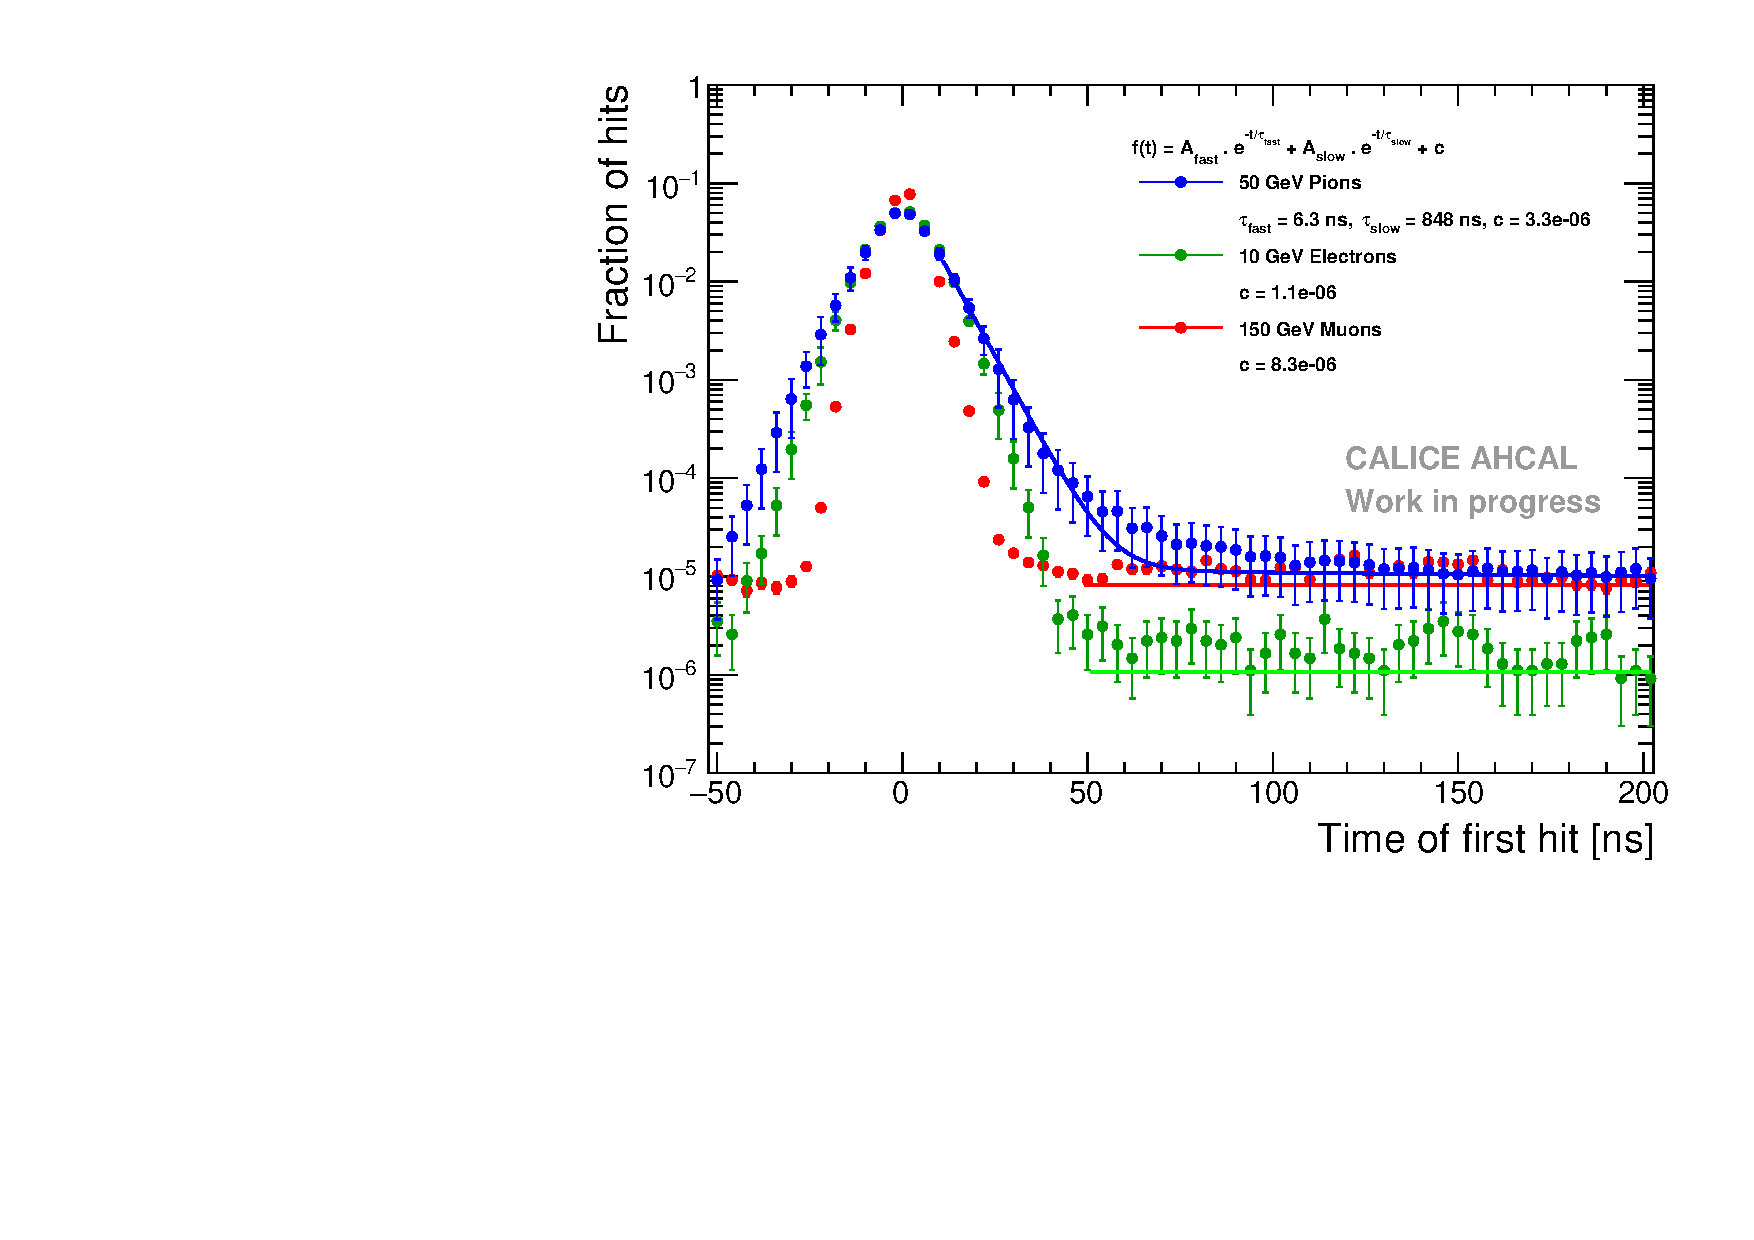
\includegraphics[width=0.6\textwidth]{chap5/fig_AHCAL_timing/Pions/Timing_dNdt_Comparison.pdf}
	\caption{Time of first hit for muons, electrons and pions in steel absorber in a range of -50 to 200 ns. The histograms are normalised to the number of events. The lines represent the fit to the data as explained in the text.}
	\label{fig:dNdt_Comparison}
\end{figure}

The figure \ref{fig:dNdt_Comparison} confirms this. Muons and electrons energy deposition are instantaneous within a certain time window centered around $t=0$ ns (determined by the intrinsic time resolution of the detector). Some isolated hits are present in the tails most likely caused by SiPM thermal noise. This gives an idea of the noise level as well as the rejection of noise in the analysis. One can remark that the noise level in electron data is lower than in the muon data. The reason is not clear and may come from the operation of the detector. Around 2.03\% of hits are after 50 ns compared to the core of the distribution between -50 and 50 ns. For electrons, only 0.37\% of hits are in the same region.
For hadron showers, the situation is different. In this case, about 1.55\% of hits are after 50 ns. Moreover, the pion data presents a higher tail between 30 to 50 ns than in the electron data. In order to characterize the distribution, a similar model of the sum of two exponentials and a contant as the T3B experiment \cite{Simon2013} is applied following the equation \ref{eq:dNdt_eq}:

\begin{equation} \label{eq:dNdt_eq}
	\frac{1}{N}\frac{dN}{dt} = A_{fast} \times e^{-\frac{t}{\tau_{fast}}} + A_{slow} \times e^{-\frac{t}{\tau_{slow}}} + c
\end{equation}

where $A_{fast}, \tau_{fast}$ and $A_{slow}, \tau_{slow}$ are the amplitudes and decays times of the modeled fast and slow component of the hadronic shower. Since the fit is performed on several orders of magnitudes, the same method that T3B has been applied for fitting. It is done in two steps. First, the slow component is fitted between 90 ns and \SI{2}{\micro\second}. Then fixing the parameters of the slow component, the fast component is fitted between 10 ns to \SI{2}{\micro\second}.
With this procedure, a fast component of $7.04 \pm 0.59$ ns and a slow component of $826 \pm 183$ ns are fitted. The fast component is in the same order of magnitude as given by T3B of 8 ns and interpreted by the evaporation neutrons energy depositions in the active medium. But due to the time resolution of the AHCAL being in the same order of magnitude, it is difficult to confirm this origin. On the other hand, the slow component is very different than in T3B (around 80 ns in steel). This may be due to the contribution of SiPM noise which reduces the sensitivity to this slow component in the shower. One can also remark that this model may be incomplete as the fitting function does match well the data in the transition region of 50 to 100 ns similar as the T3B data. The table \ref{table:dNdt_fit} sums up the fitted results.

\begin{table}[htb!]
	\centering
	\caption{Summary of the fit results in figure \ref{fig:dNdt_Comparison}.}
	\label{table:dNdt_fit}
	\begin{tabular}{@{} lccc @{}}
		\hline
		Parameter & Muon & Electron & Pion \\
		\hline
		$\tau_{fast}$ [ns] & - & - & $7.04 \pm 0.59$ \\
		$\tau_{slow}$ [ns] & - & - & $826 \pm 183$ \\
		$c$ & $(7.91 \pm 0.09) \times 10^{-6}$ & $(1.20 \pm 0.02) \times 10^{-6}$ & $(3.38 \pm 0.56) \times 10^{-6}$ \\
		\hline
	\end{tabular}
\end{table}

The energy dependence of the timing of hits has been studied in a second step as shown in figure \ref{fig:Energy_Comparison}. It shows the mean time of first hit taken between [-50, 200] ns as function of the hit energy for muon, electron and pion beams. For muons and electrons, no dependence with energy is observed as expected as all hits are prompt. For pions, the situation is different. A delay of 2-3 ns at 0.5 MIP is observed and decreases down to 0-1 ns above 1 MIP. For higher pion energies than 10 GeV, a dip in the distribution can be observed between 0.5 and 1.5 MIP. This effect is most likely due to an over-correction of the data with the number of triggered channels in a chip. In principle, it should follow the same shape as for 10 GeV pions as there should be no dependency with beam energy.

\begin{figure}[htbp!]
	\centering
	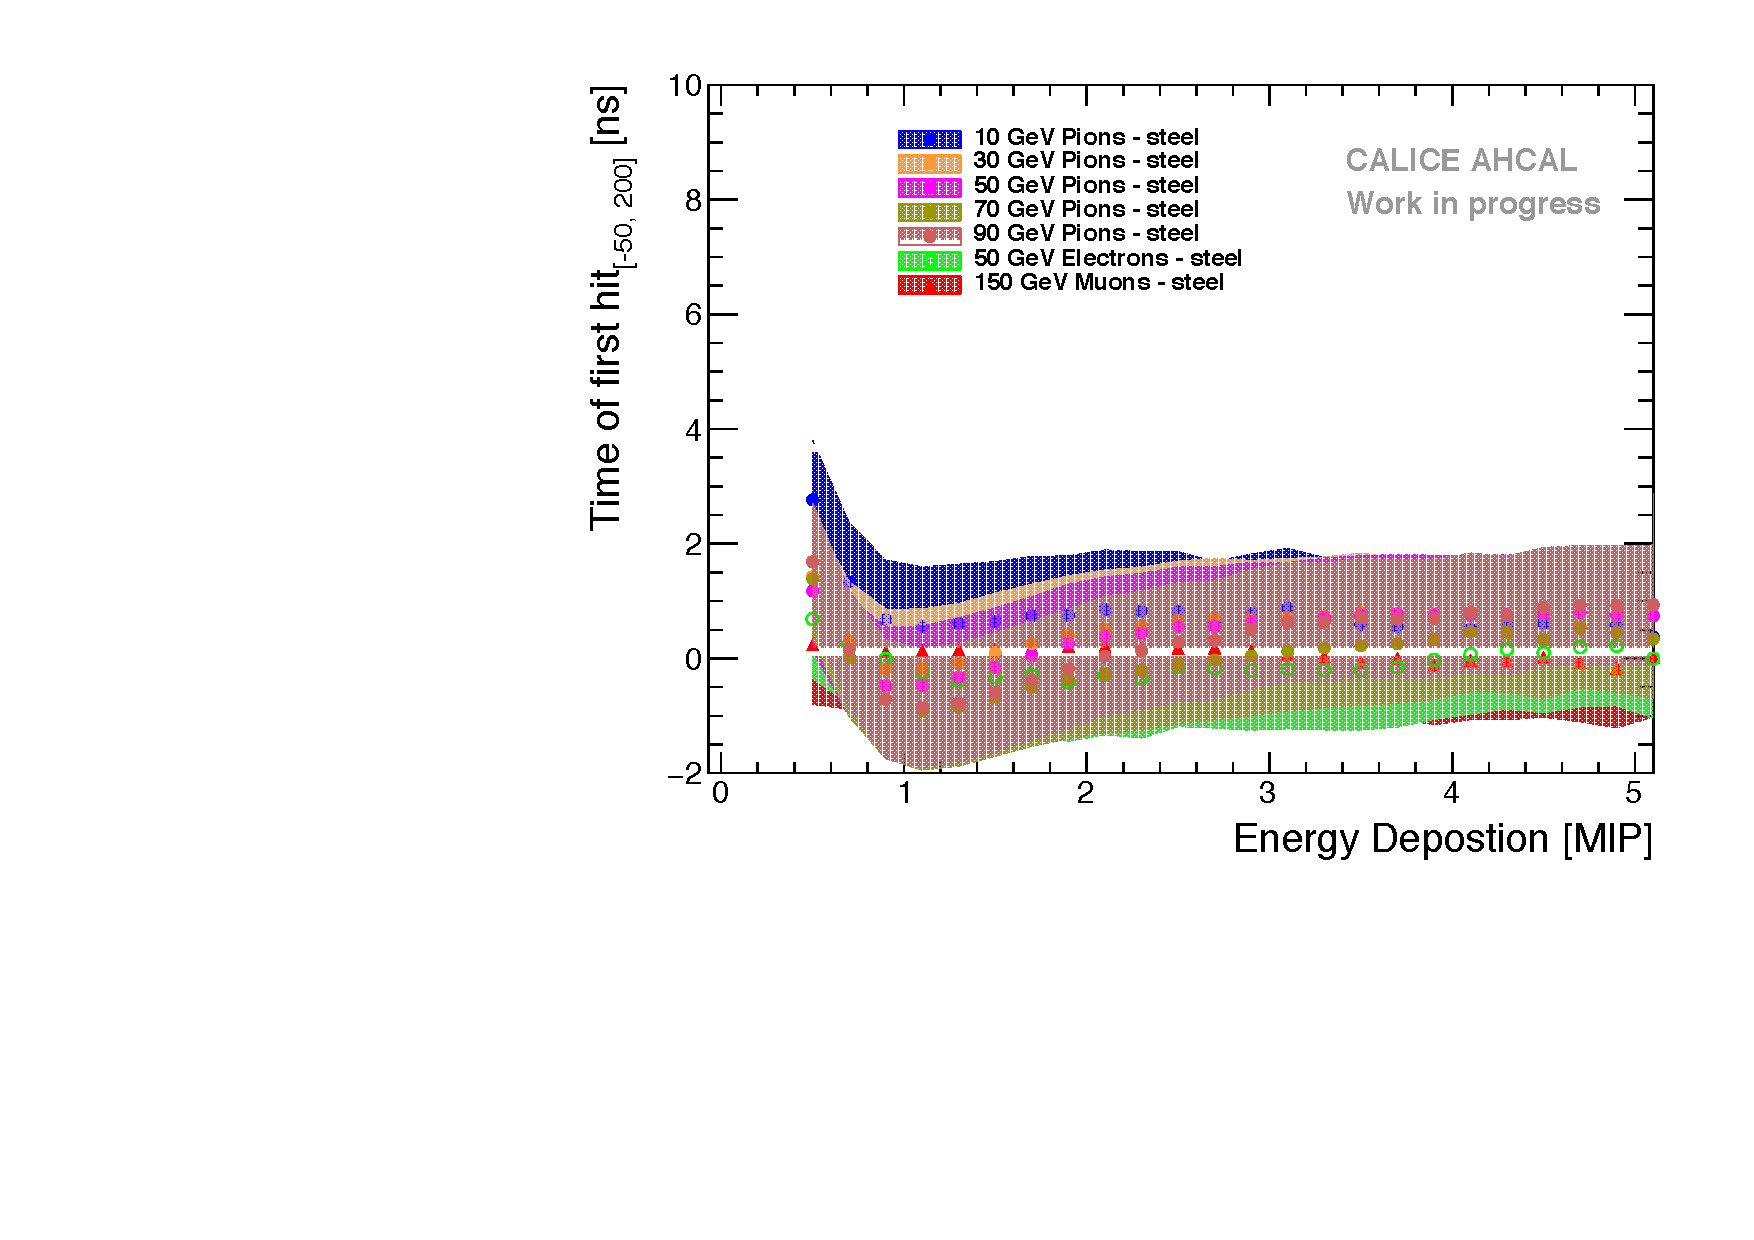
\includegraphics[width=0.6\textwidth]{chap5/fig_AHCAL_timing/Pions/Timing_Energy_Comparison_ShortAsymRange.pdf}
	\caption{Time of first hit as function of the hit energy for muons, electrons and pions in steel absorber in a range of -50 to 200 ns.}
	\label{fig:Energy_Comparison}
\end{figure}

This figure demonstrates that low energy hits are responsible for delayed deposition most likely by low energy neutron from capture and spallation processes. Higher energy deposits occurs mostly in the prompt part of the hadron shower.

\section{Radial dependence of timing profiles}

As shown in the previous subsection, the prompt part of the shower is dominated by EM subshowers and relativistic particles. The delayed part is coming from mostly evaporation and spallation low energy neutrons. It is expected that the former is concentrated near the shower axis as for the latter, it is spread out laterally as these neutrons can travel far away in the calorimeter before interacting. This is investigated by looking at the mean time of first hit as a function of the distance to the shower center of gravity defined in the [x,y] plane. This is shown in figures \ref{fig:Radius_Comparison_SSF} and \ref{fig:Radius_Comparison_BL} for the small layers from 3 to 10 and the big layers from 11 to 14 separately.

\begin{figure}[htbp!]
	\begin{subfigure}[t]{0.5\textwidth}
		\centering
		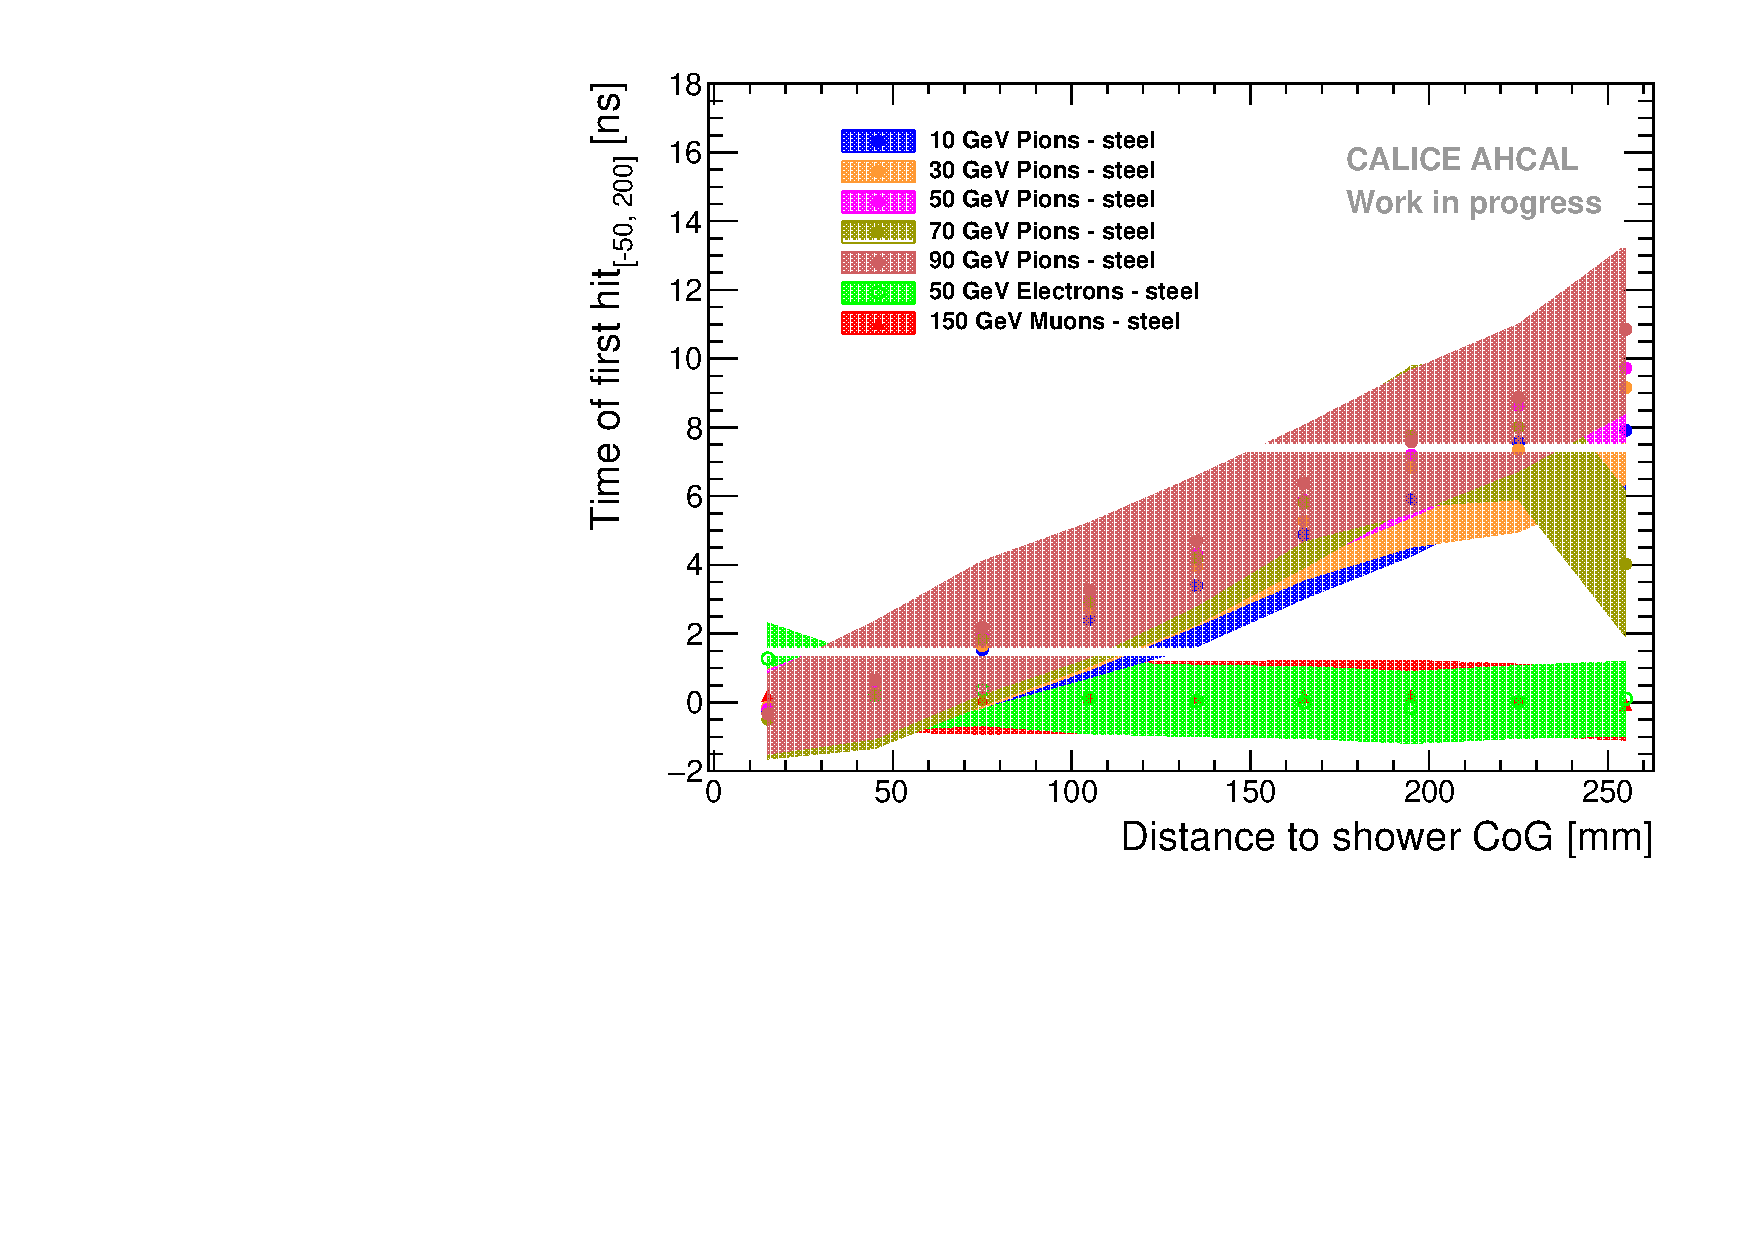
\includegraphics[width=1\textwidth]{chap5/fig_AHCAL_timing/Pions/Timing_Radius_Comparison_ShortAsymRange_SSF.pdf}
		\caption{Small layers from 3 to 10.}\label{fig:Radius_Comparison_SSF}
	\end{subfigure}
	\hfill
	\begin{subfigure}[t]{0.5\textwidth}
		\centering
		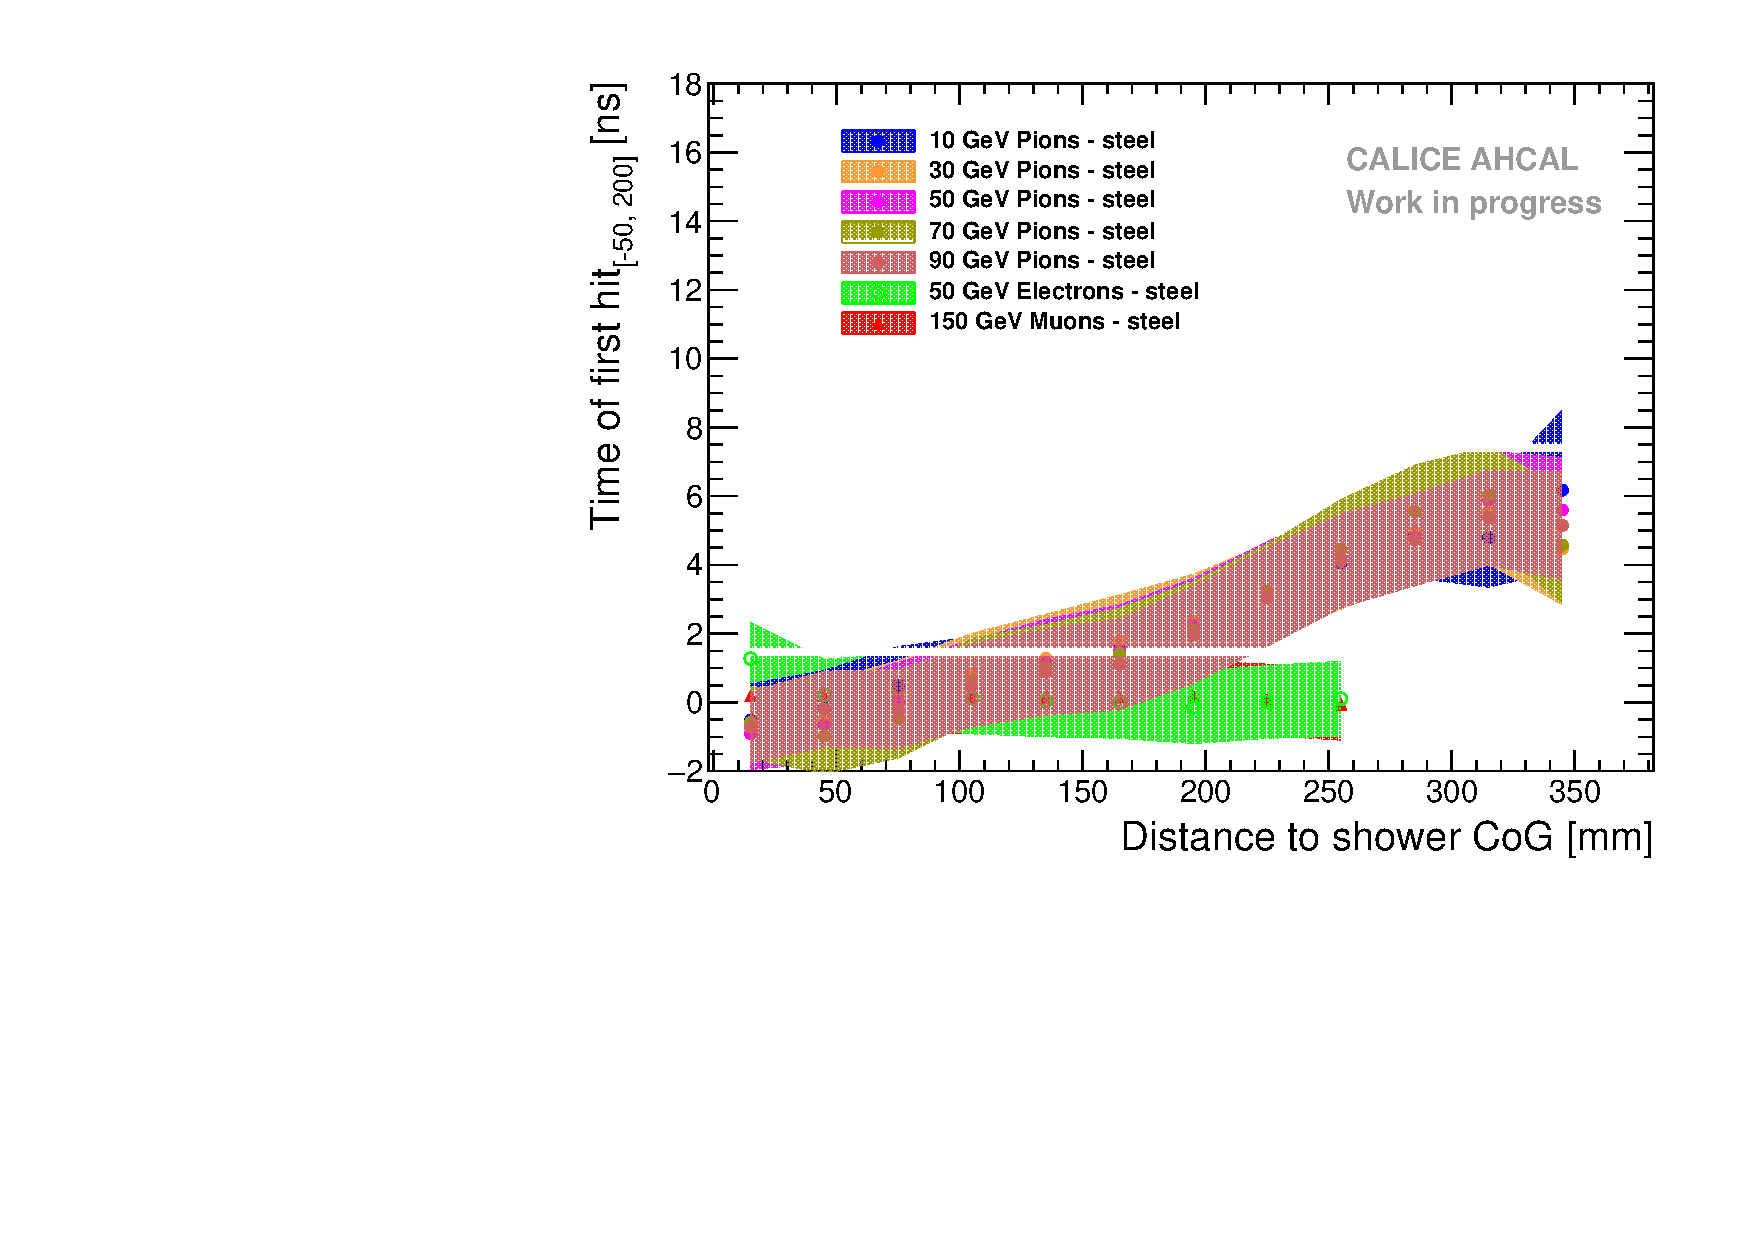
\includegraphics[width=1\textwidth]{chap5/fig_AHCAL_timing/Pions/Timing_Radius_Comparison_ShortAsymRange_BL.pdf}
		\caption{Big layers from 11 to 14.}\label{fig:Radius_Comparison_BL}
	\end{subfigure}
	\caption{Radial shower timing profile of the time of first hit for muon, electron and pion beams. The left plot shows the timing profile for the small layers and the right profile shows the timing profile for big layers. The explanation for the separation is described in the text. The systematics are shown by the color bands.}
	\label{fig:RadialTiming}
\end{figure}

For muons and electrons, the mean time of the first hit does not vary with the increase of radius showing that the processes involved are prompt and independant of the position. On the contrary for hadronic showers, it shows an increase with the distance to the shower axis for both type of boards, though the slopes are different with the small layers presenting a steeper slope. This is consistant with the expectation of the core of the shower depositing promptly most of the energy via EM subshowers and relativistic particle near the shower axis. This is followed by a hadronic halo which contributes to delayed signals by mainly neutron-induced processes. For the small layers, the time of first hit varies between 0 ns at small radius and 10 ns at 25 cm. For the big layers, it varies between 0 ns near the shower axis, 4 ns at 25 cm and 6 ns at 35 cm. This shows a relative difference between both distributions. This is thought to come from the fact that different parts of the shower are sampled in the front / back of the calorimeter respectively depending on the position of the start of the shower.

To confirm this, I investigated the time of first hit as function of the radius to the shower axis at constant distance between the layer investigated and the first hard interaction (FHI) layer of the hadronic shower. First, a small algorithm for a shower start finder to find the layer of the first hard interaction had to be written. This is based on previous work \cite{CaN026} with slight modifications due to the fact that few layers in the front of the detector present a bad performance. The basics of the algorithm was to find the primary track and check the number of hits between layer $i$ and $i+1$. This number was chosen to be $>6$. If an event was found in this case, a check on the length of the track was performed and it was required to be $>3$ hits in a track. A simple check on the performance of the algorithm was done by looking at the difference between the reconstructed layer of the FHI and the Monte-Carlo truth as well as the correlation between both. This is shown in figures \ref{fig:Diff_FHI_RecoMC} and \ref{fig:Corr_FHI_RecoMC}. The performance of the algorithm is good enough in order to get a good estimate of the FHI layer and has a small tendency to reconstruct the FHI at deeper layer.

\begin{figure}[htbp!]
	\begin{subfigure}[t]{0.5\textwidth}
		\centering
		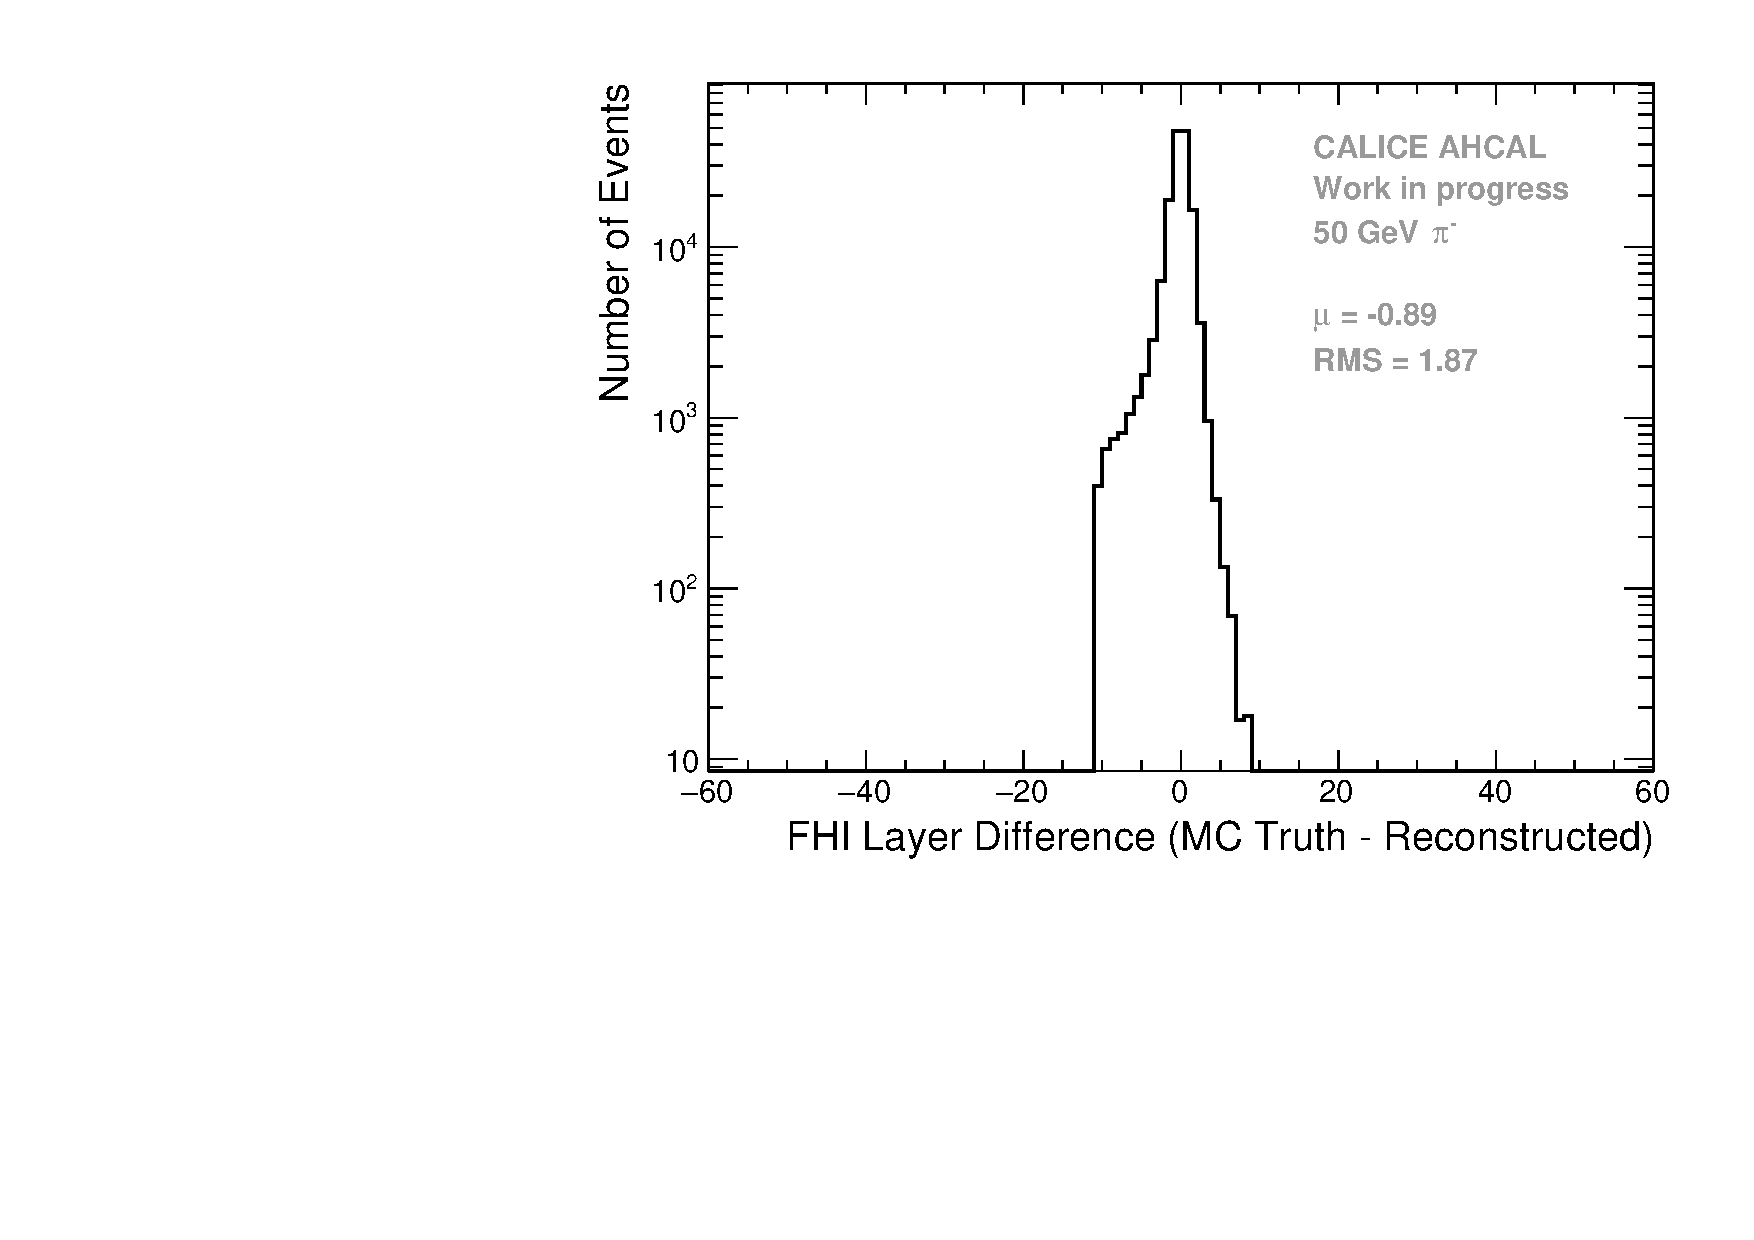
\includegraphics[width=1\textwidth]{chap5/fig_AHCAL_timing/Pions/ShowerStart_Difference_noOptimisation.pdf}
		\caption{Difference between reconstructed FHI and MC truth layer.}\label{fig:Diff_FHI_RecoMC}
	\end{subfigure}
	\hfill
	\begin{subfigure}[t]{0.5\textwidth}
		\centering
		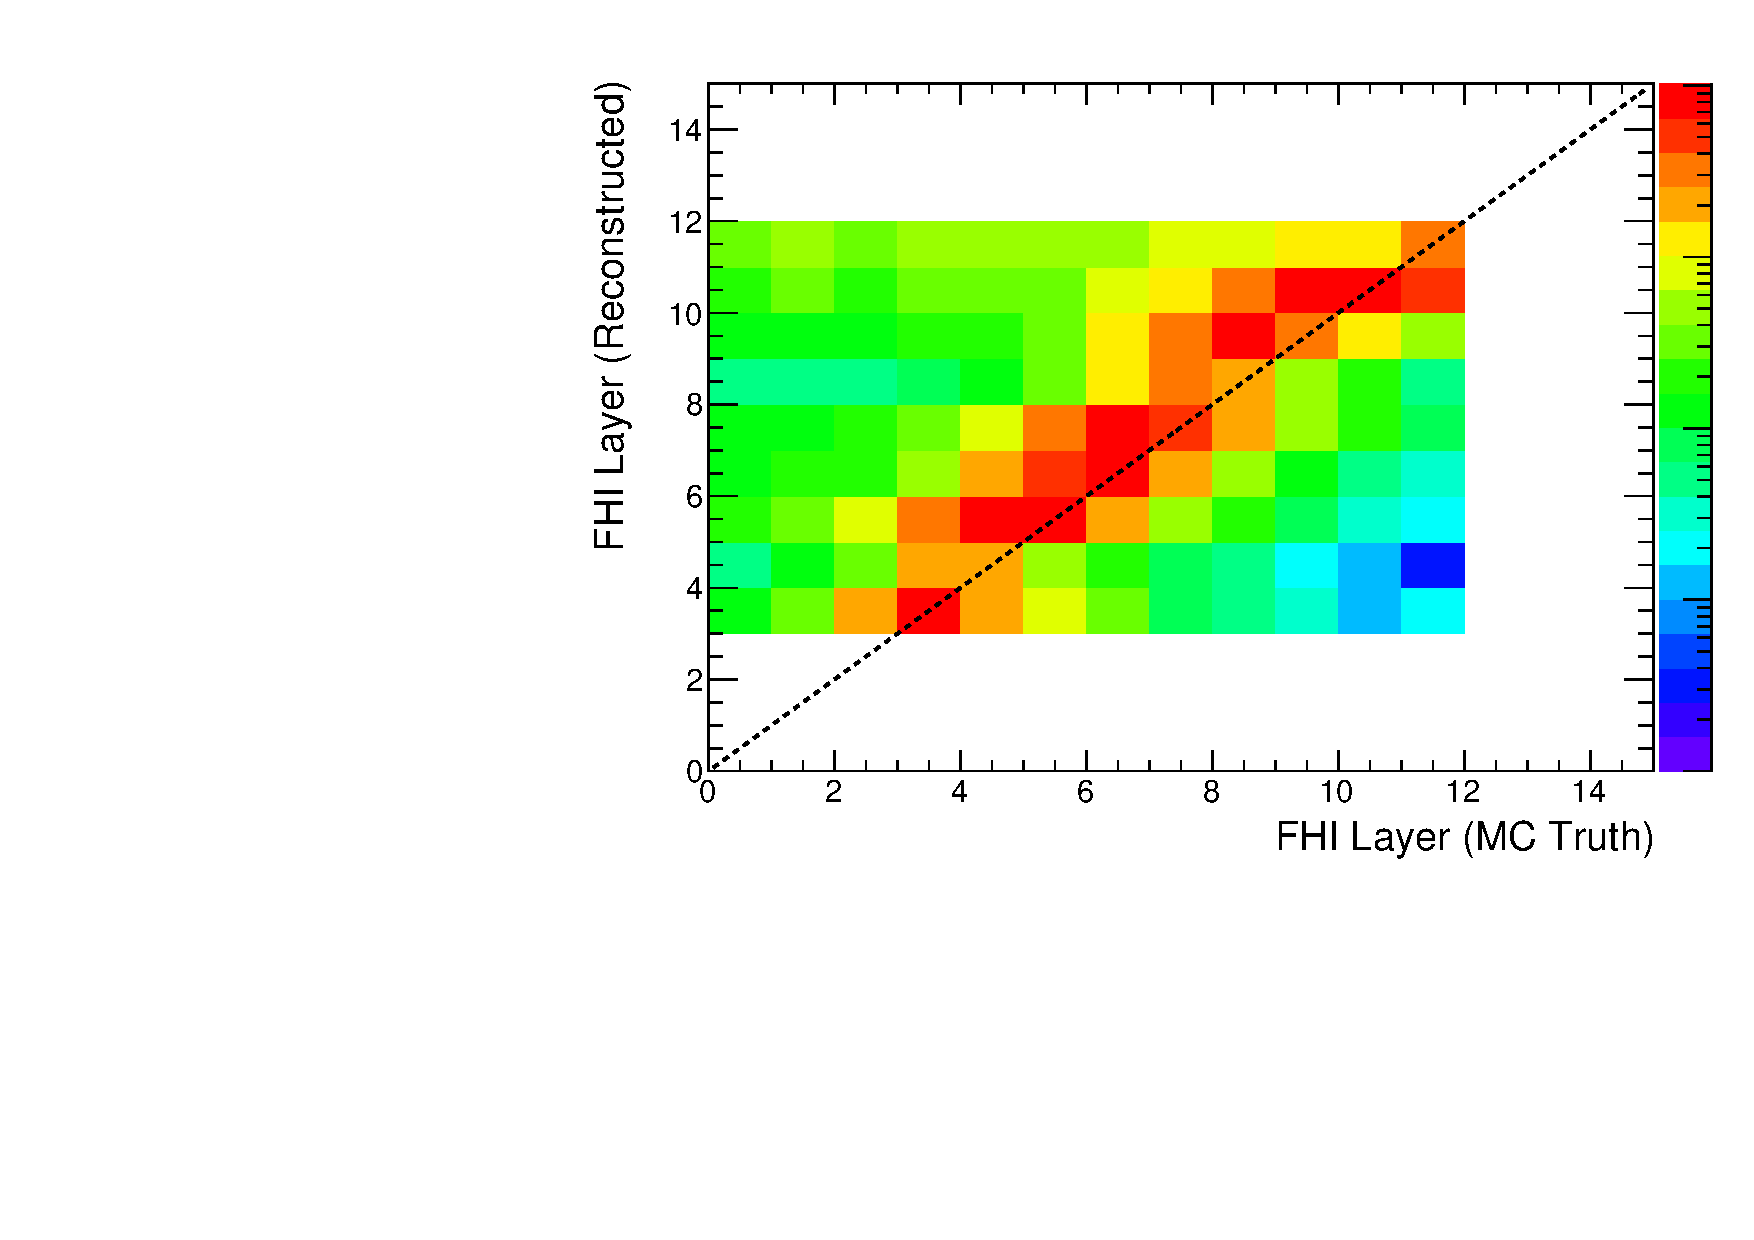
\includegraphics[width=1\textwidth]{chap5/fig_AHCAL_timing/Pions/ShowerStart_Difference_noOptimisation_2D.pdf}
		\caption{Correlation between reconstructed FHI and MC truth layer.}\label{fig:Corr_FHI_RecoMC}
	\end{subfigure}
	\caption{Performance check of the FHI algorithm in the AHCAL detector. The left plot shows the difference between the reconstructed FHI and the MC truth. The distribution is slightly decentred at -0.81 with a RMS of 1.87. The right plot shows the correlation between them. The black line represent a guide line for a perfect correlation.}
	\label{fig:FHIAlgo}
\end{figure}

Looking back at the data, it is expected that with a constant distance between the reconstructed FHI and the layer investigated that there will be the same dependence of the mean time of the hit as function of the radius as the same part of the shower would be sampled. Or that inversely by looking at a fixed layer for different FHI layer, the expected behavior would be a change in the slope of the time of first hit as function of the radius to the shower axis. The figure \ref{fig:Radius_FHI} and \ref{fig:Radius_FHI_Fixed} is an attempt at this.

\begin{figure}[htbp!]
	\begin{subfigure}[t]{0.5\textwidth}
		\centering
		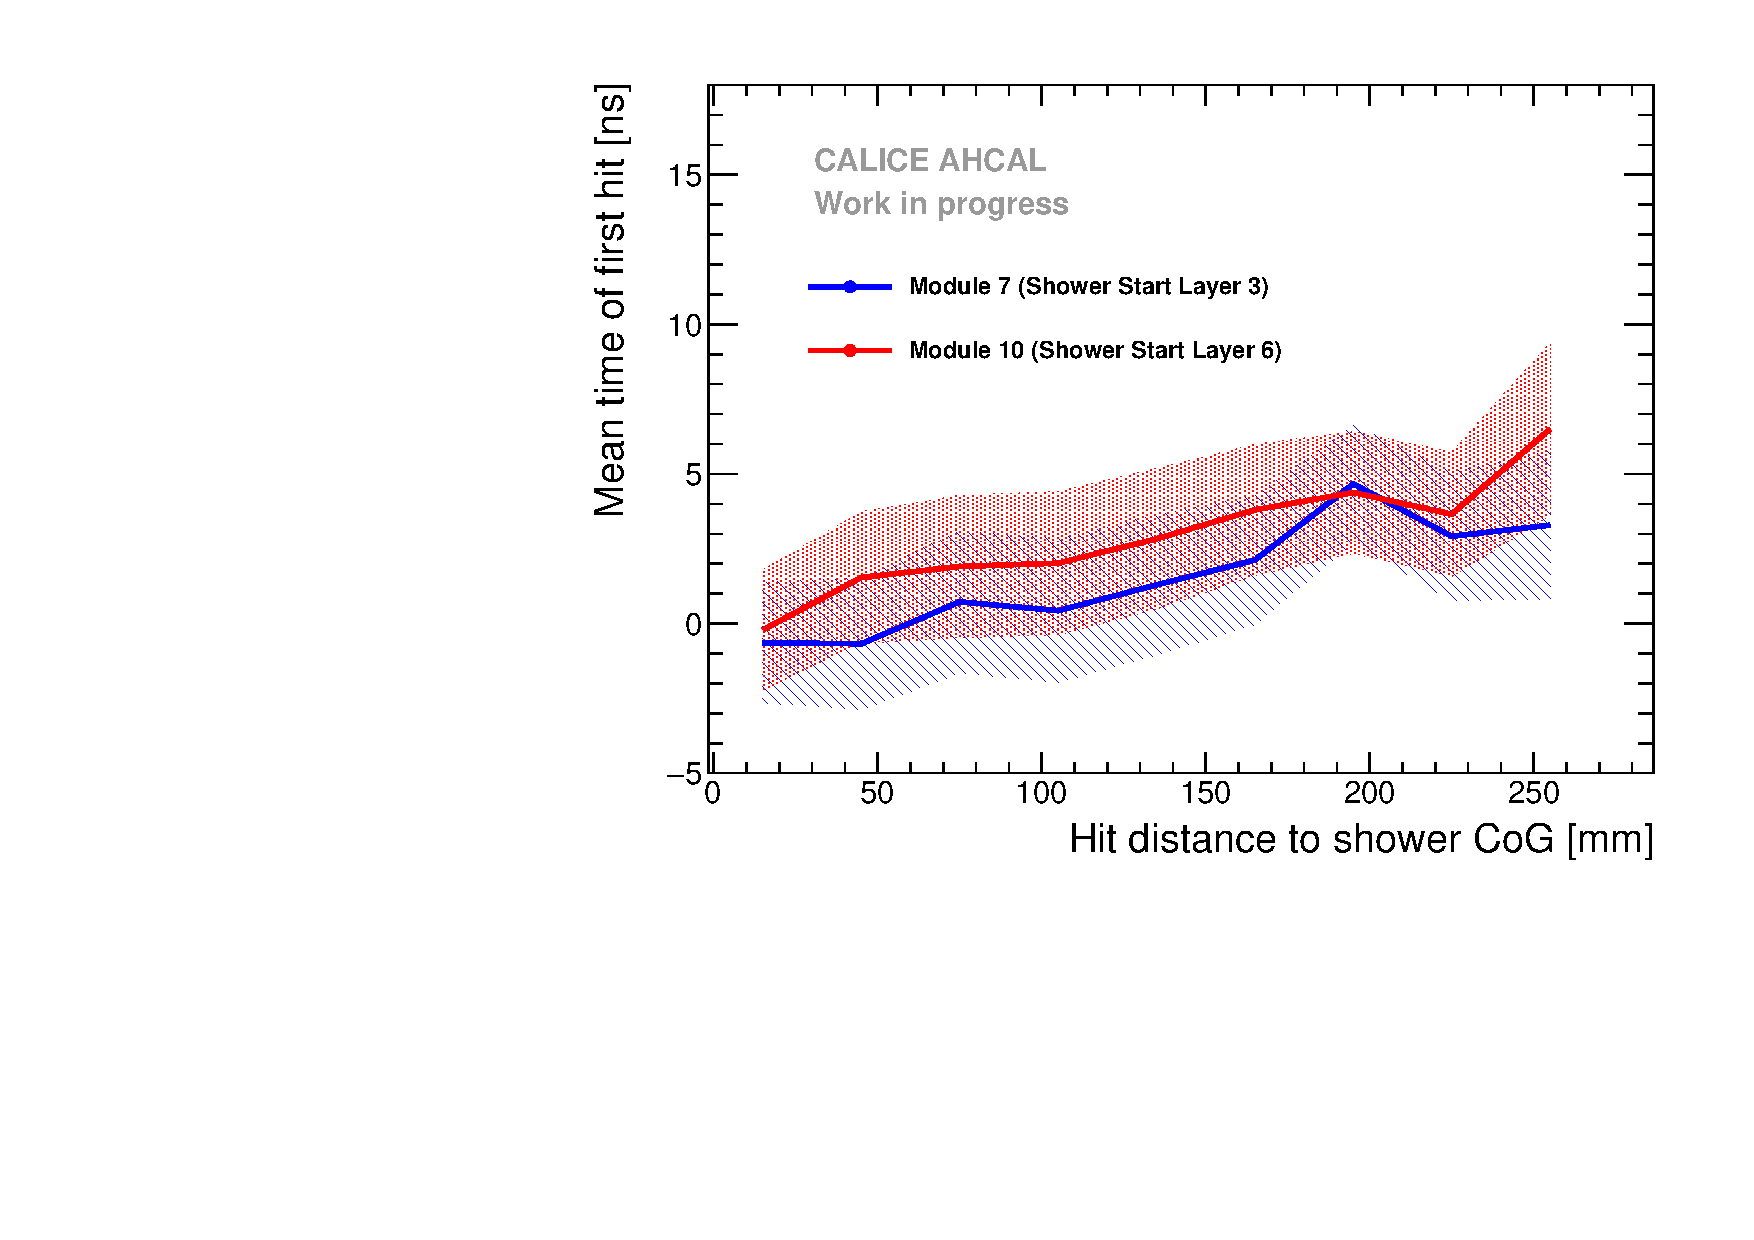
\includegraphics[width=1\textwidth]{chap5/fig_AHCAL_timing/Pions/Timing_Radius_Comparison_ShortAsymRange_ShowerStart.pdf}
		\caption{Fixed FHI-layer distance case.}\label{fig:Radius_FHI}
	\end{subfigure}
	\hfill
	\begin{subfigure}[t]{0.5\textwidth}
		\centering
		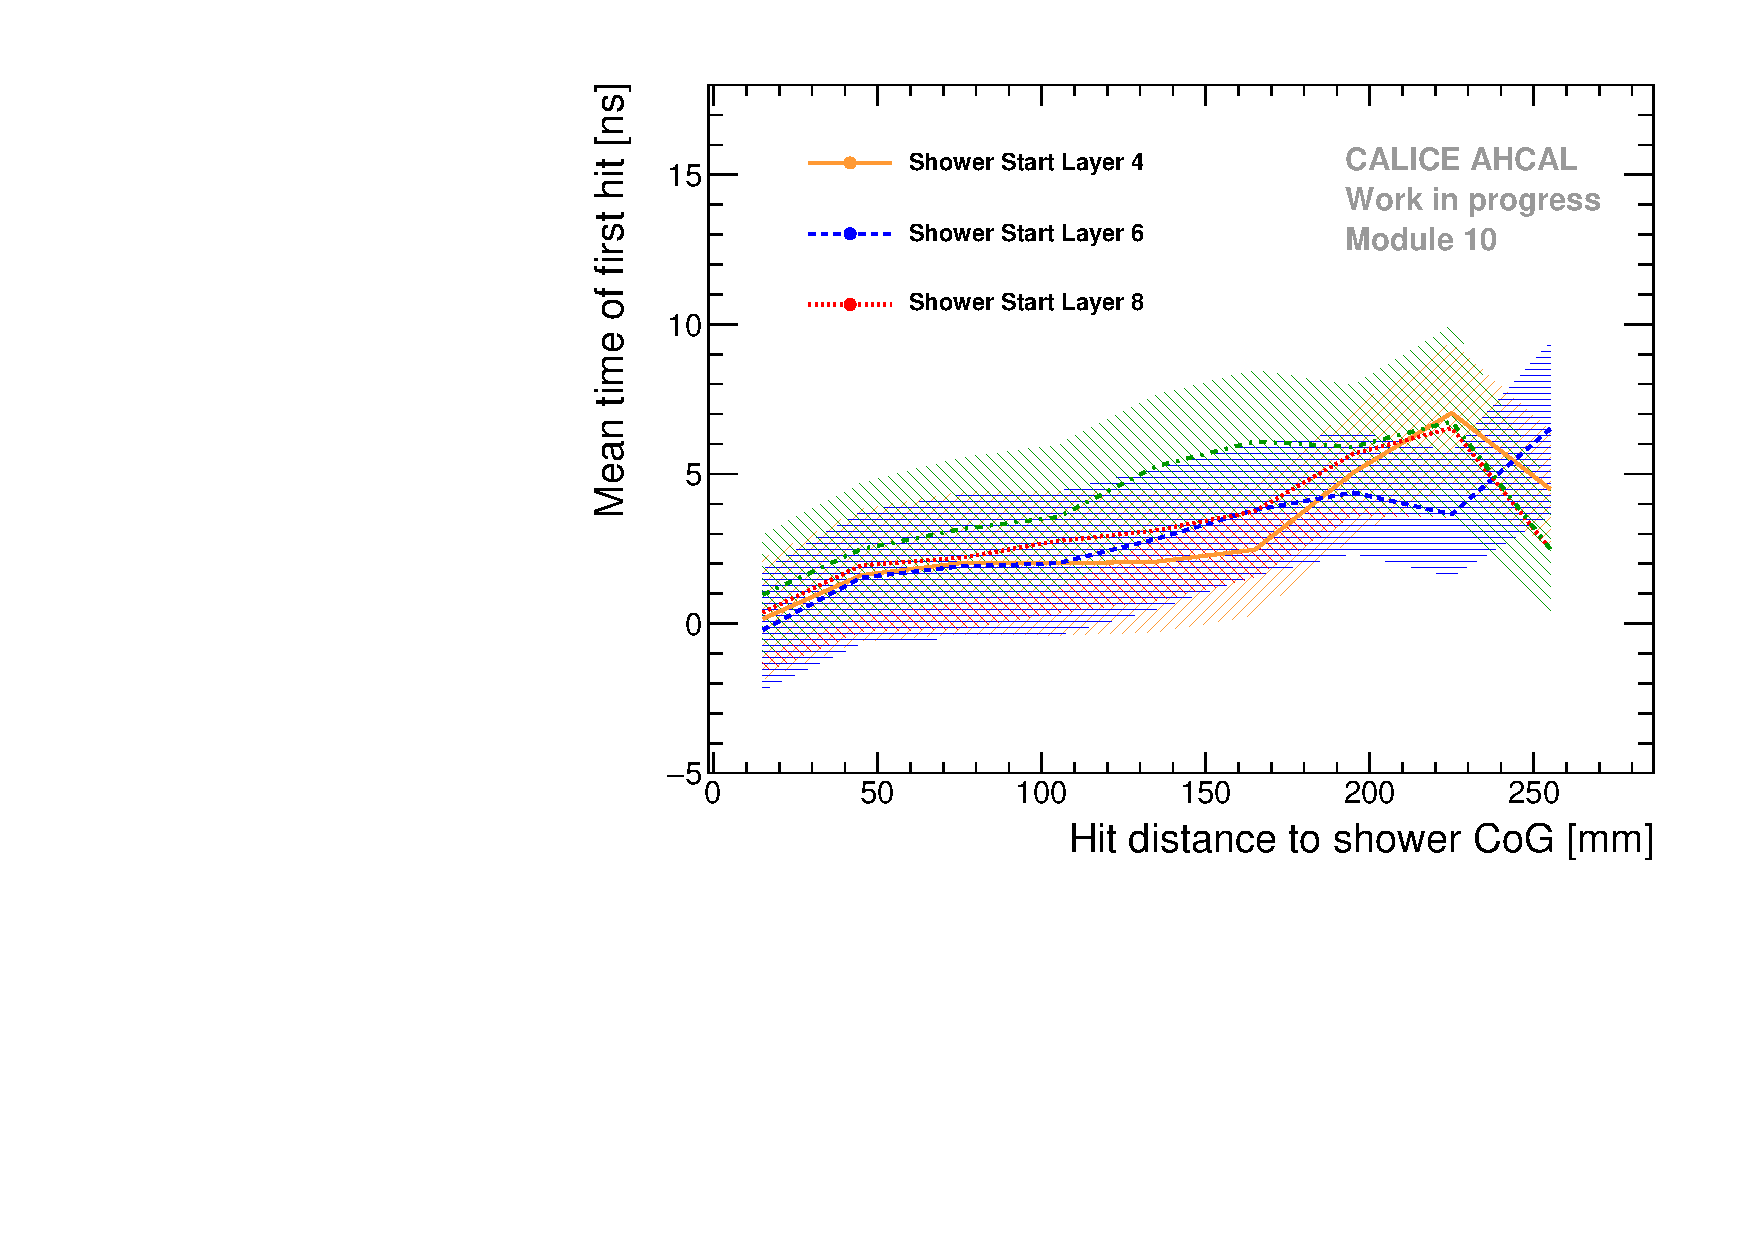
\includegraphics[width=1\textwidth]{chap5/fig_AHCAL_timing/Pions/Timing_Radius_Comparison_ShortAsymRange_ShowerStart_FixedModule.pdf}
		\caption{Fixed layer with difference FHI case.}\label{fig:Radius_FHI_Fixed}
	\end{subfigure}
	\caption{Investigation of the difference of the shape of the radial timing distribution between small and big layers. The left plot shows the timing profile of layer 7 and 10 selecting events only where the difference between the reconstructed FHI layer and the observed layer is 4. The right plot shows the time profile of layer 10 for events with different reconstructed FHI.}
	\label{fig:Radius_FHI}
\end{figure}

The data seems to shows that by fixing the distance between the FHI and the layer, that the time of first hit displays the same slope within the systematic uncertainties. Also on the other side, looking at a fixed layer in this case layer 10, it seems that there is a trend of an increase of the slope of the distribution as function of the reconstructed FHI within the systematics. Unfortunately due to the small amount of data available as well as the unusability of more layers of the detector, it is difficult to confirm this observation and would need more investigation in a new testbeam campaign with a full equipped prototype.

\section{Longitudinal dependence of timing profiles}

The longitudinal dependence of time was also looked at. It is expected that the further you are in the calorimeter that more low energy neutrons contributes to the energy deposition thus enhancing the late tail. The figure \ref{fig:Depth_Comparison} shown the mean time of first hit as function of the layer position for muon, electron and pion beams.

\begin{figure}[htbp!]
	\begin{subfigure}[t]{0.5\textwidth}
		\centering
		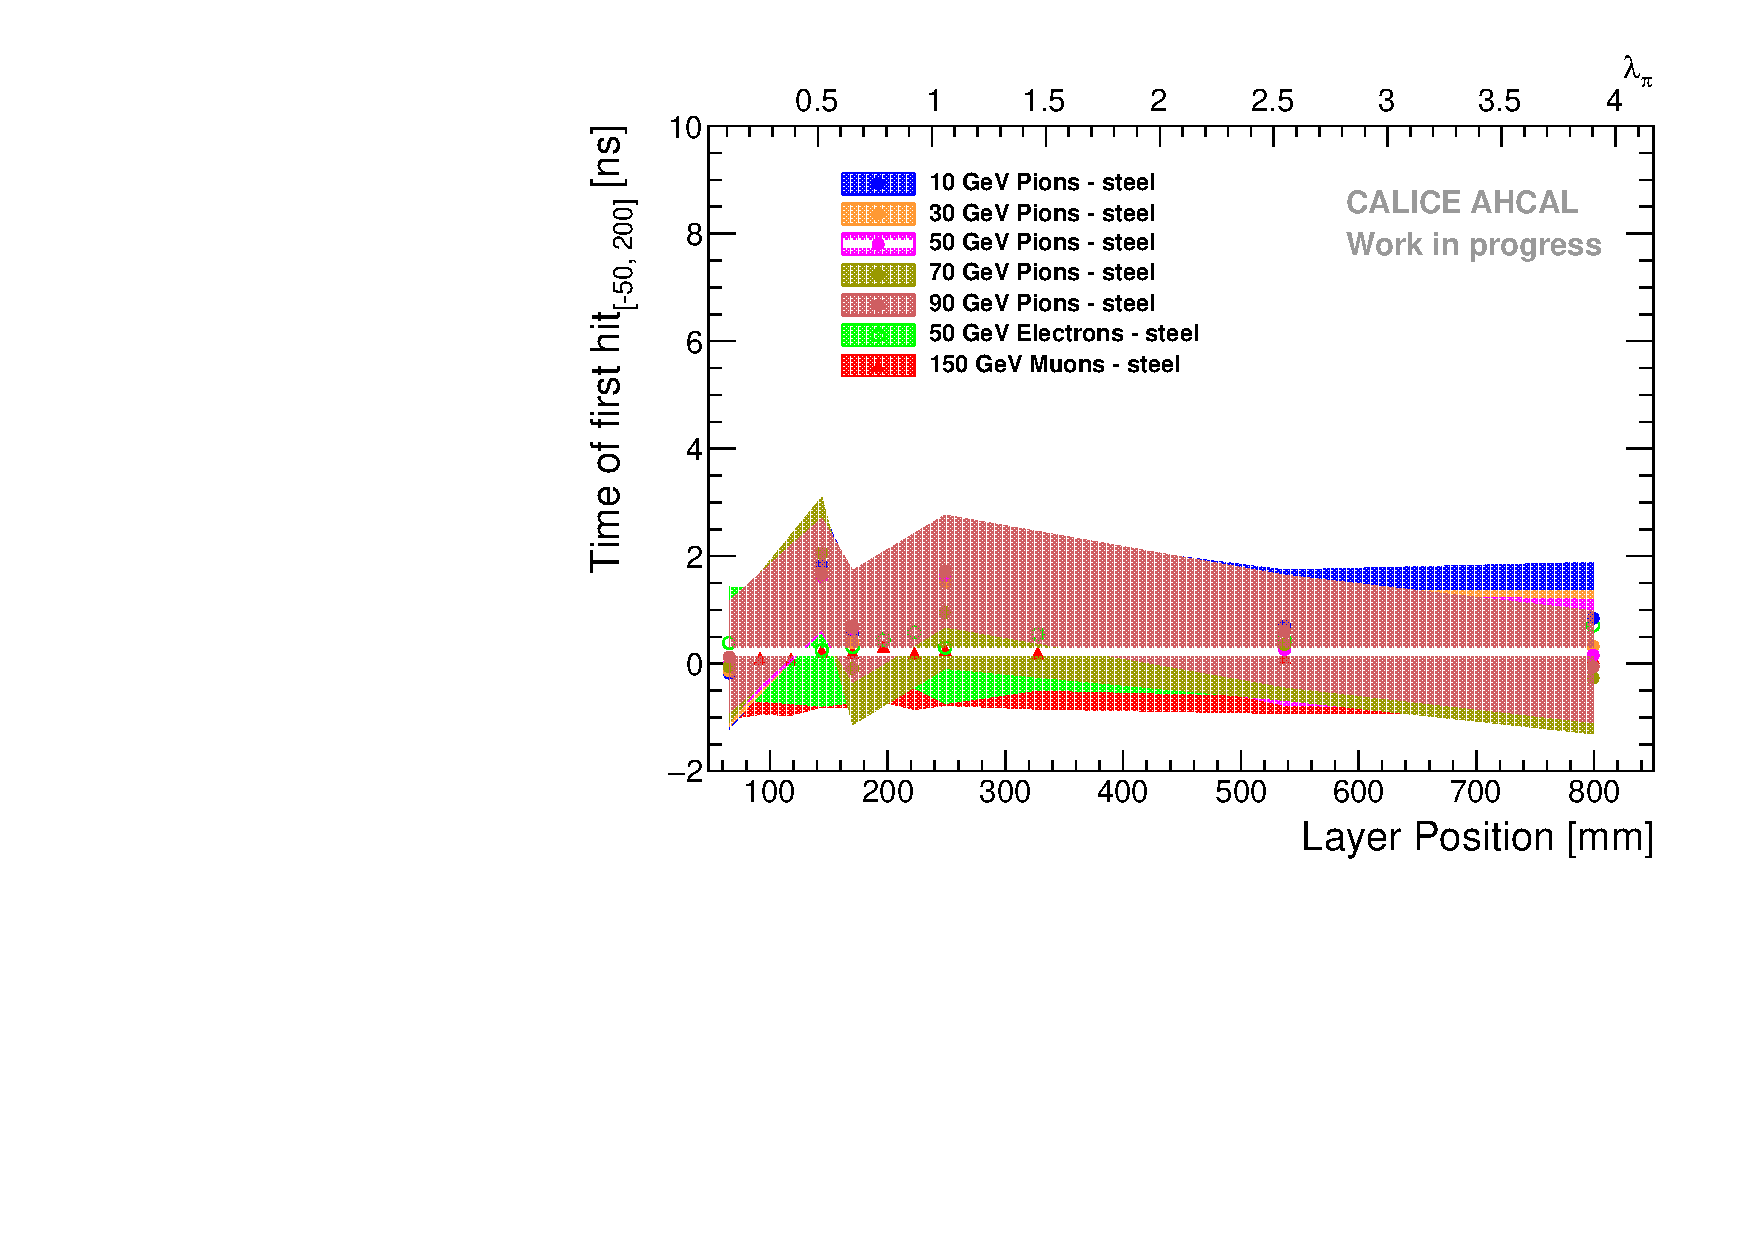
\includegraphics[width=1\textwidth]{chap5/fig_AHCAL_timing/Pions/Timing_Depth_Comparison_ShortAsymRange.pdf}
		\caption{Time of first hit as function of the layer position.} \label{fig:Depth_Comparison}
	\end{subfigure}
	\hfill
	\begin{subfigure}[t]{0.5\textwidth}
		\centering
		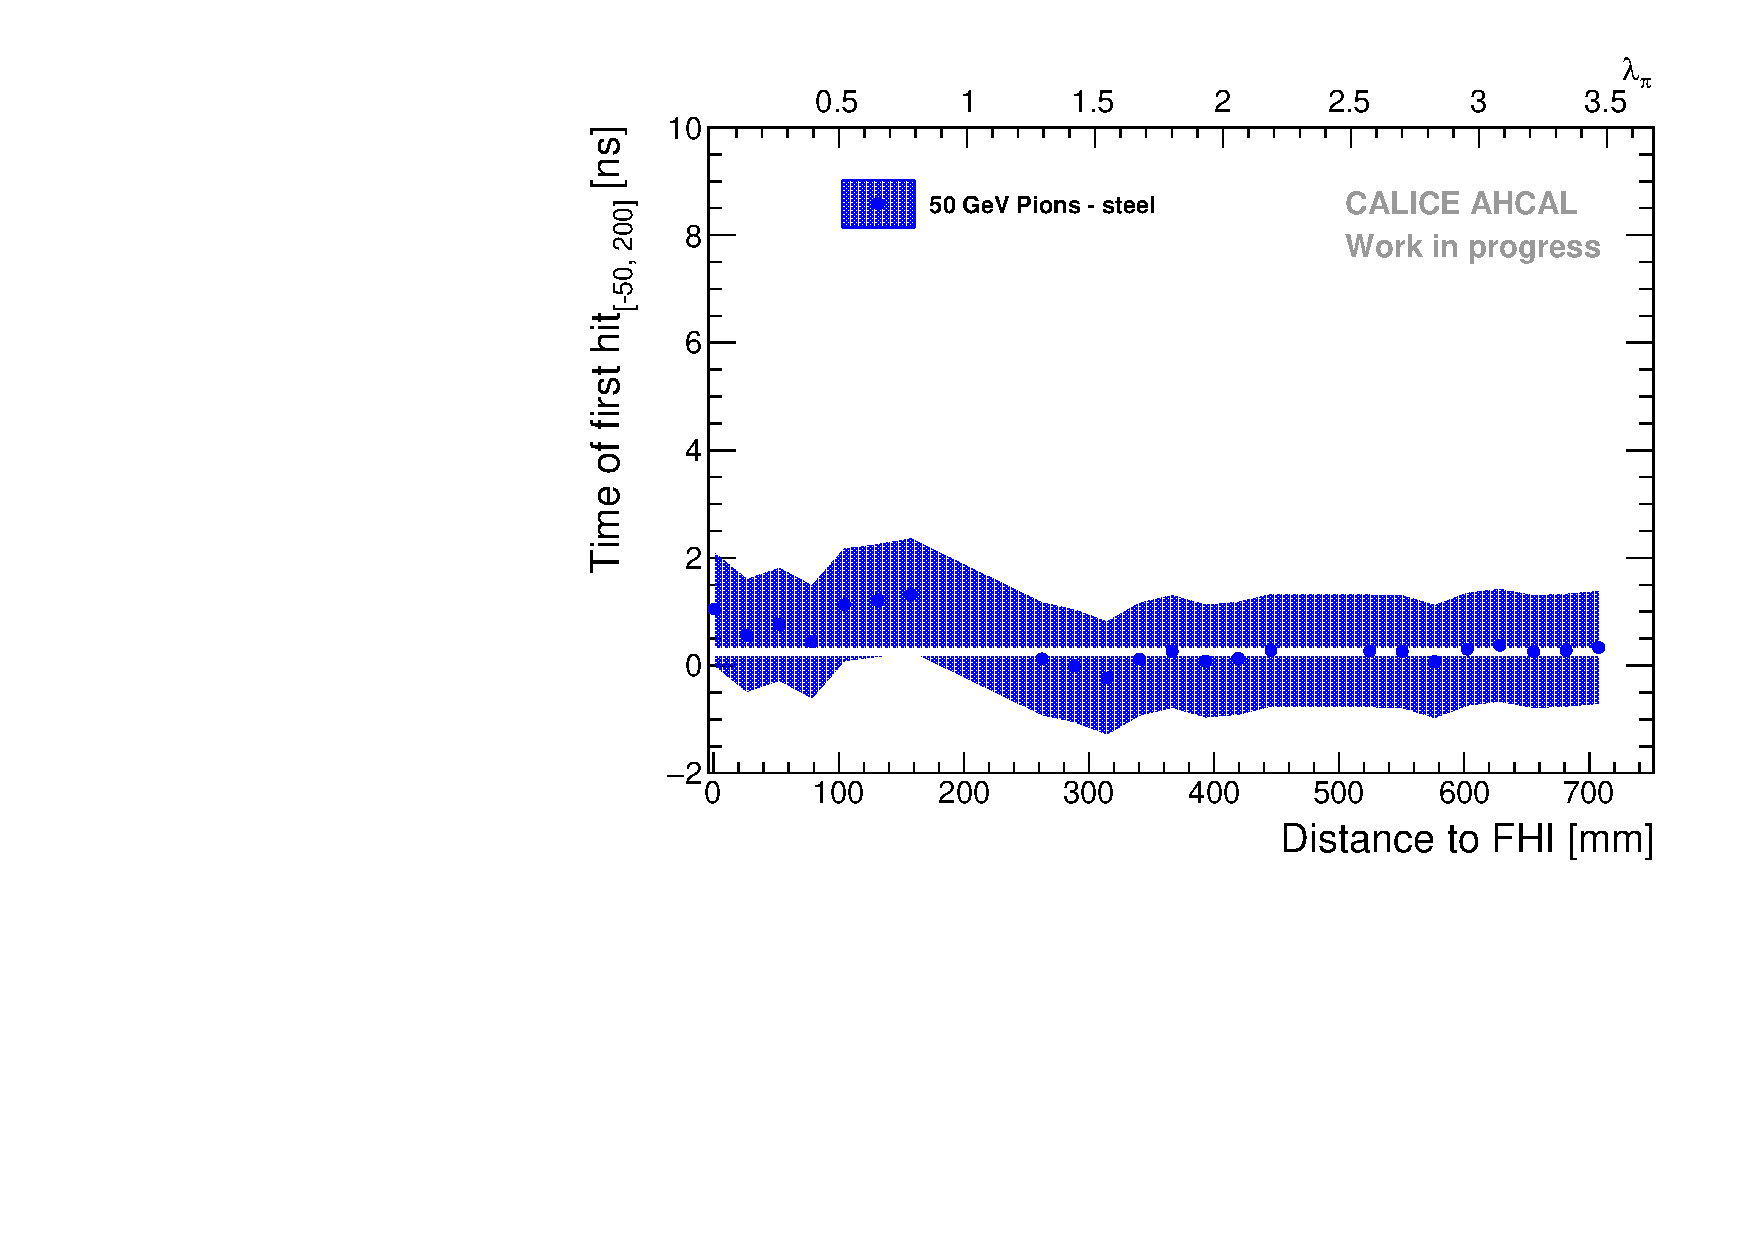
\includegraphics[width=1\textwidth]{chap5/fig_AHCAL_timing/Pions/Timing_Depth_Comparison_ShortAsymRange_ShowerStart.pdf}
		\caption{Time of first hit as function of the distance to the FHI.}\label{fig:Depth_Comparison_FHI}
	\end{subfigure}
	\caption{The left plot shows that all distributions are compatible with a flat distribution for the time of first hit as function of the layer position. The right plot shows the same as function of the distance to the reconstructed FHI.}
	\label{fig:DepthProfile}
\end{figure}

It seems that the observation in the data is compatible with no increase of the time with the layer depth within systematics. This may be due to the fact that the sensibility to this late component is suppressed by the time resolution of the calorimeter as well as the systematic errors. An attempt to get a better sensitivity was to look at the mean time of first hit as function of the depth from the reconstructed FHI as shown in figure \ref{fig:Depth_Comparison_FHI}. Same conclusion within systematics this is compatible with a flat distribution around $t=0$.

\section{Time correlations between layers}

The advantage of this studied prototype over T3B is the possibility to investigate the possible time correlations between layers. This has been looked at as shown in figures \ref{fig:Time_Corr_short} and \ref{fig:Time_Corr_long} for the 50 GeV pion sample. For this, the data below 50 ns is ignored as only the tail of the timing distributions is interresting. Two types of correlations was investigated, short and long. The procedure is done by looking at each hits in layer $i$ and checking in an area of 2-3 tiles behind in layer $i+1$ for a hit. If a hit is found, both times are correlated. If more than one hit is found, the closest to the hit in layer $i$ is taken. For the short correlation, the layers 6 and 7 were chosen. As for the long, the layers 13 and 14 were selected. These were chosen due to the fact that few layers were working properly. It is not very clear what to expect in these cases except that for the short one, a possible correlation would be visible due to the proximity of the layers.

\begin{figure}[htbp!]
	\begin{subfigure}[t]{0.5\textwidth}
		\centering
		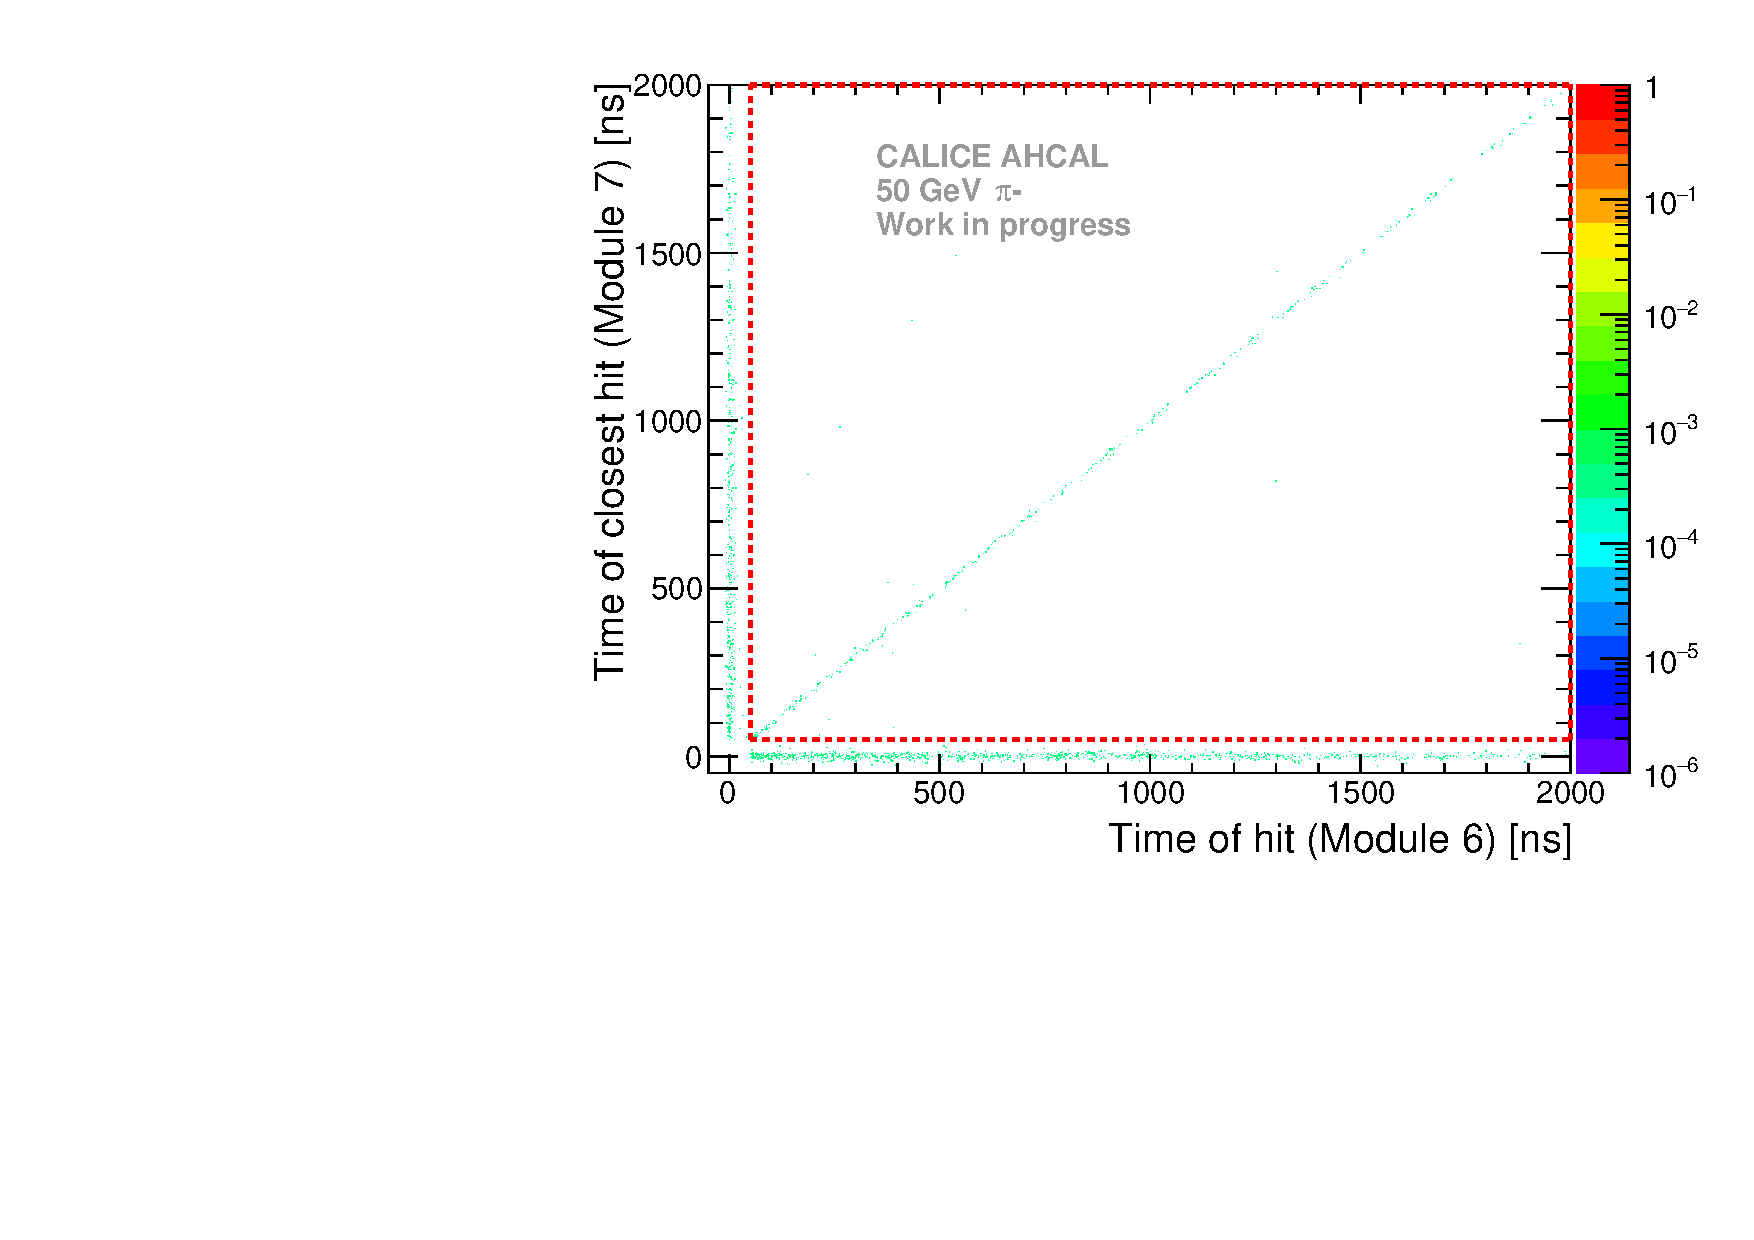
\includegraphics[width=1\textwidth]{chap5/fig_AHCAL_timing/Pions/Time_Correlation_short.pdf}
		\caption{Time correlation between layer 6 and 7 for 50 GeV pions.} \label{fig:Time_Corr_short}
	\end{subfigure}
	\hfill
	\begin{subfigure}[t]{0.5\textwidth}
		\centering
		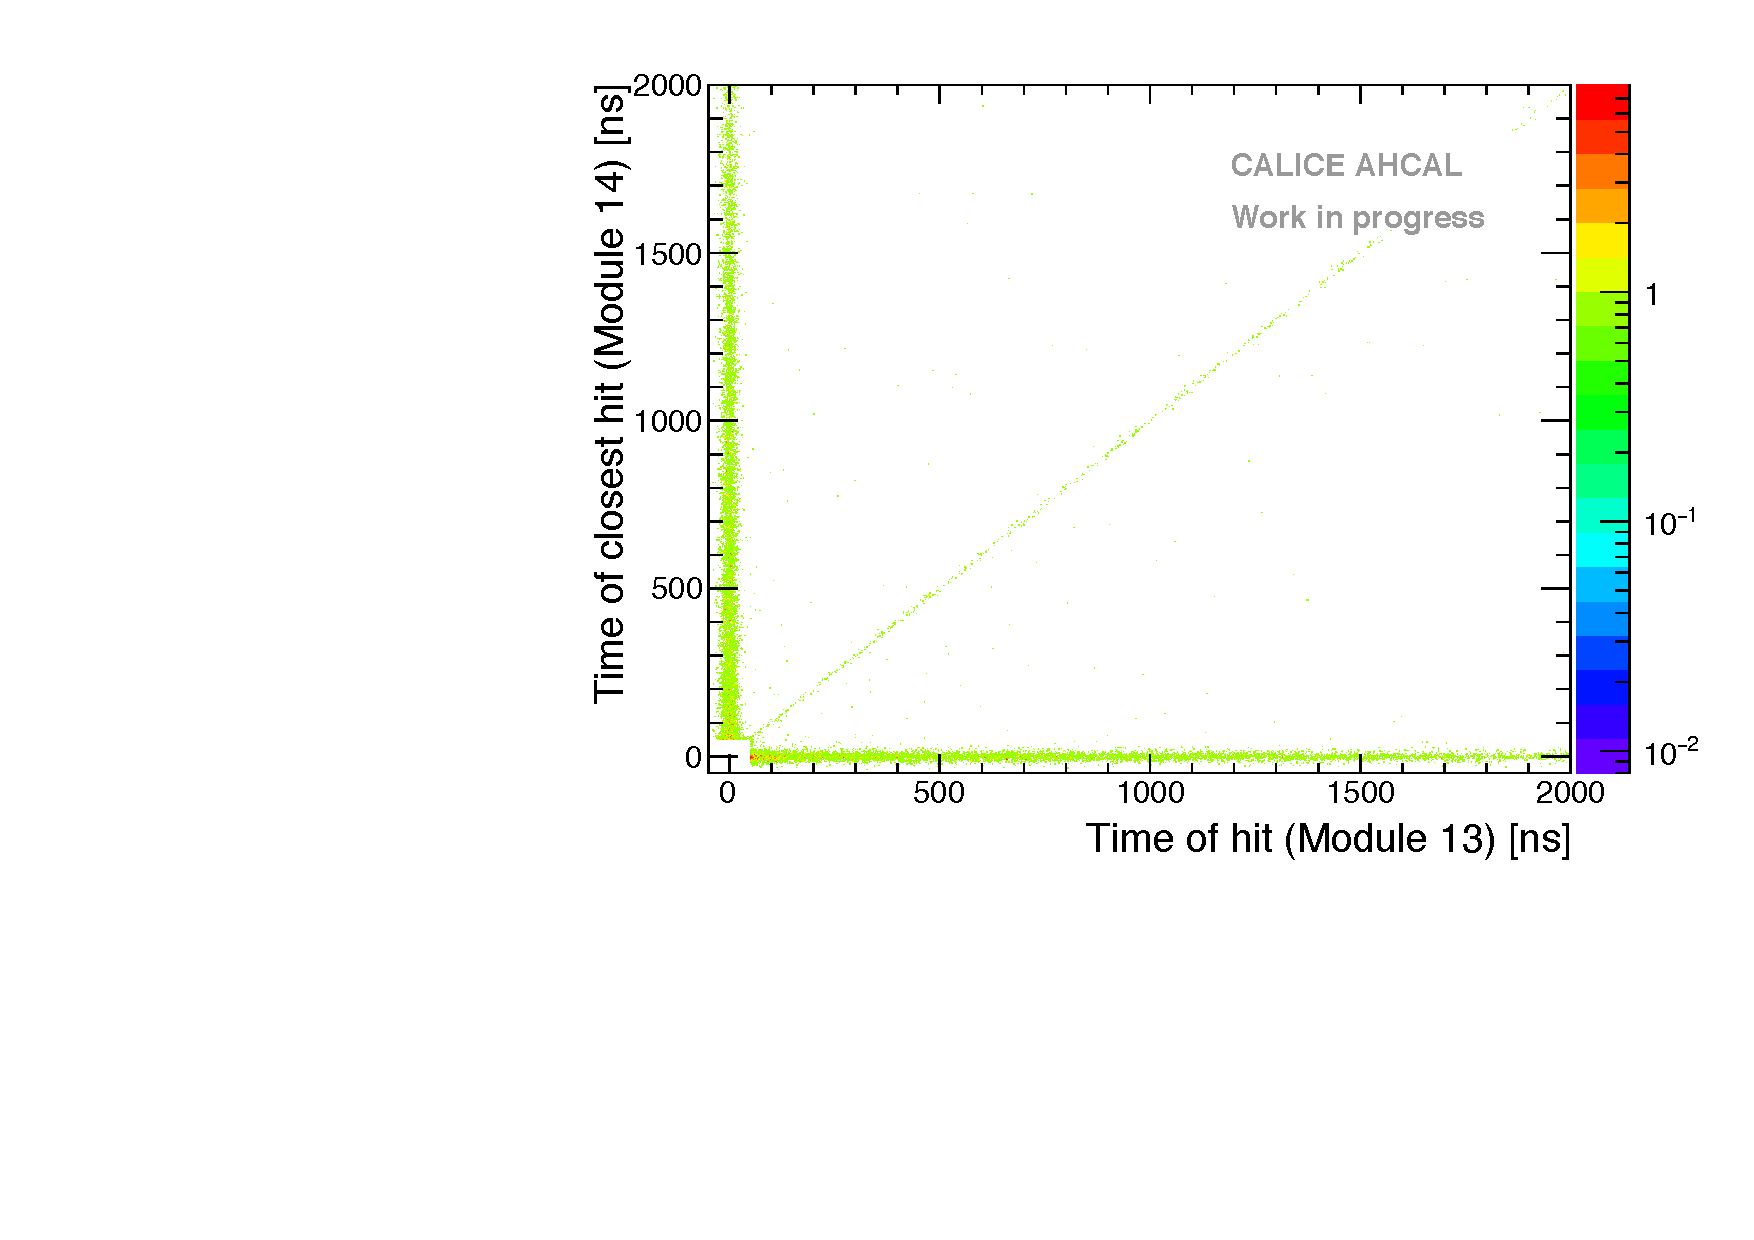
\includegraphics[width=1\textwidth]{chap5/fig_AHCAL_timing/Pions/Time_Correlation_long.pdf}
		\caption{Time correlation between layer 13 and 14 for 50 GeV pions.}\label{fig:Time_Corr_long}
	\end{subfigure}
	\caption{The left plot shows the time correlation between layer 6 and 7 separated by 1 $X_0$. The right plot shows the time correlation for layers 13 and 14 separated by 1 $\lambda_{\pi}$. Both plots show a visible time correlation.}
	\label{fig:TimeCorrelation}
\end{figure}

The figures show that a correlation is visible in both cases in the data. To quantify this, the ratio $R$ of the number of hits per time bin between 50 ns and \SI{2}{\micro\second} and the total number of entries per bin $N_{tot}$ in the histogram is calculated:

\begin{equation}
	R = \frac{\int_{50 ns}^{2 \mu s} \int_{50 ns}^{2 \mu s} \frac{dN_i(t)}{dt_i} \frac{dN_j(t)}{dt_j} dt_i dt_j}{N_{tot}}
\end{equation}

The results show that 18.14\% of the entries are on the diagonal for the short correlation. This could be indeed possible due to the proximity of the layer and may come from the prompt and fast component of the hadron shower. For the long correlation, 3.24\% of the entries are on the diagonal. This represent a substential amount of hits that are correlated. This is not clear the origin of this correlation but it may come from the fact that the suppression of the multiple particle events that is not suppressed enough and decrease the sensitivity.

\section{Comparison to simulation}

In this section, the data collected is compared to \geant simulations using different hadronic models as explained in chapter \ref{chap:G4Simulation}. The figures \ref{fig:dNdt_SimData_Comparison} show the time distribution of first hits compared with three different physics lists for pion beams ranging from 10 to 90 GeV.

From 10 to 50 GeV, QGSP\_BERT\_HP reproduces well the distribution. Over 50 GeV, the late tail is well described by the distribution but between 50 and 100 ns is not well reproduced and under-estimated. This may be just an effect remaining in the data that has not been completely removed by corrections. QBBC tends to over-estimate slightly the late tail by around a factor 2. This somehow contradicts the observations made in the T3B experiment were QBBC agreed well with the time distribution. It may be related to the use of different \geant versions. For all distributions, QGSP\_BERT over-estimate the tail of the distribution by around a factor 10. For the core of the distribution under 50 ns, generally all physics lists describe relatively well the distribution within systematics.

The figures \ref{fig:Energy_SimData_Comparison} show the mean time of first hit as function of the hit energy. For 10 GeV pion, the simulation reproduces well the data within the systematics. For higher energies, a difference is visible in the region 0.5 to 1.5 MIP where the simulation is above the data. This is believed due to an over-correction of the data that shifts down the distribution. Above around 2 MIPs, the data and simulations agree well. QBBC and QGSP\_BERT seems higher in general over the full energy range showing that without precision neutron tracking, late depositions may be produced in too much quantities though this is within systematics of the data.

The radial profile of pion showers is also compared to simulations as shown on figures \ref{fig:Radius_SSF_SimData_Comparison} and \ref{fig:Radius_BL_SimData_Comparison}. For the small layers, the physics lists QBBC and QGSP\_BERT\_HP reproduce well the data within systematics. QGSP\_BERT agrees well under 10 cm and starts to deviate up to 4-6 ns at 23 cm. Concerning the big layers, over the full energy range, QGSP\_BERT\_HP physics list agrees the best with the data. QBBC and QGSP\_BERT agree with data up to around 10 cm radius and then over-estimate the mean time of first hit. The difference with the data varies between 1 ns to 3-4 ns between 10 cm to 35 cm radius. This confirms that without precision neutron tracking, too many late energy depositions are created that are spread far away from the shower axis.

As the calorimeter is equipped with many layers, the longitudinal timing profile was also compared to simulations. As in the data, the mean time of first hit is compatible with a flat distribution around $t=0$. All simulations agree with the data within systematics. The timing resolution of the AHCAL may be too high in order to be sensitive to any small changes of the mean time over the calorimeter depth.

Finally, as in data, time correlations between layers were looked at for different physics lists as shown in figures \ref{fig:Corr_Mokka_Simulation}. In the same way, the number of correlated hits was calculated and it is summed up in table \ref{table:Correlation_DataSim}. Looking at the number, there is a large discrepency between data and simulation. In general, simulations posseses less correlated hits than in data for both types. DD4hep also has slightly less correlated hits than in Mokka but is within statistical uncertainties. The reason for the discrepency is not yet clear though it may come from the selection of the data that may be not good enough to reject multi-particle events thus providing more correlated hits than observed in simulation. More data is required in order to understand the origin of such correlations.

\begin{table}[htb!]
	\centering
	\caption{Summary of number of correlated hits. The top number is for Mokka simulations, the bottom one is for DD4hep.}
	\label{table:Correlation_DataSim}
	\begin{tabular}{@{} |l|cc| @{}}
		\hline
		Type & Short [\%] & Long [\%] \\
		\hline
		Data & 18.14 & 3.24\\
		\hline
		\multirow{2}{*}{QGSP\_BERT} & 3.93 & 0.66\\ & 2.28 & 0.50\\
		\hline
		\multirow{2}{*}{QGSP\_BERT\_HP} & 4.01 & 0.72\\ & 2.24 & 0.53\\
		\hline
		\multirow{2}{*}{QBBC} & 3.98 & 0.70\\ & 2.29 & 0.53\\
		\hline
	\end{tabular}
\end{table}

\section{Summary and Outlook}

The understanding of the time structure of hadronic showers and the level of accuracy reflected in \geant simulations is highly relevant for calorimeters at future (linear) collider experiments. This can be applied for conditions with high level of background such as $\gamma\gamma \rightarrow hadrons$ or high repetition rates experiments to remove out-of-time pile-up events.

The AHCAL testbeam at CERN in July 2015 was focused to address this, with steel absorber and closed to the ILD detector design, by collecting data from muon, electron and pion beams. The AHCAL technological prototype was equipped with 14 layers using scintillator tiles as active material readout by SiPMs to provide radial and longitidual sampling of showers with high granularity and ns-scale time resolution. For the first time, time study of hadronic showers was done to a large scale using integrated readout electronics.
In this analysis, the time calibration procedure of the AHCAL was presented. A time resolution in the order of 5 ns is achieved for a muon beam. Due to an electronic effect, a time resolution of 8 ns is achieved for electron and pion beams.

Studying hadronic showers, the data shows that late deposition are concentrated at low hit energies below 1.5 MIPs in iron. Theses hits are mostly at a great distance from the shower axis in contrary with the electromagnetic sub-showers and relativistic hadrons that a predominant near the shower axis. Timing correlations between layers has also been investigated. Correlations are visible at short range as well as long range in different proportions in the data.

The comparison of detailled simulations with data has been performed. It shows that in general, the simulation reproduces well the data within the systematics. The tracking of low energy neutrons in the HP package or other implementations like in QBBC show that they are needed to reproduce well the tail of the data where without it is generally over-estimated. Time correlations are reproduced somewhat in simulation but the proportion of hits in data and simulation differ quite significantly. This may be due to the selection of the data that does not reject efficiently multi-particle events and would need more data and investigations to understand their origin.

The running mode in Testbeam does not reflect the time resolution that would be accessible in ILC running mode. By extrapolation, a time resolution of the order of 1 ns would be optained. The use of timing information could be a powerful tool to have to help in separating nearby showers in case of very busy events, for example a $ttH$ event. It could be used in a software compensation way by using timing bins differentiating electromagnetic subshowers or relativistic hadrons and the hadronic late component, and weight them accordingly.

\begin{figure}[htbp!]
	\begin{subfigure}[t]{0.5\textwidth}
		\centering
		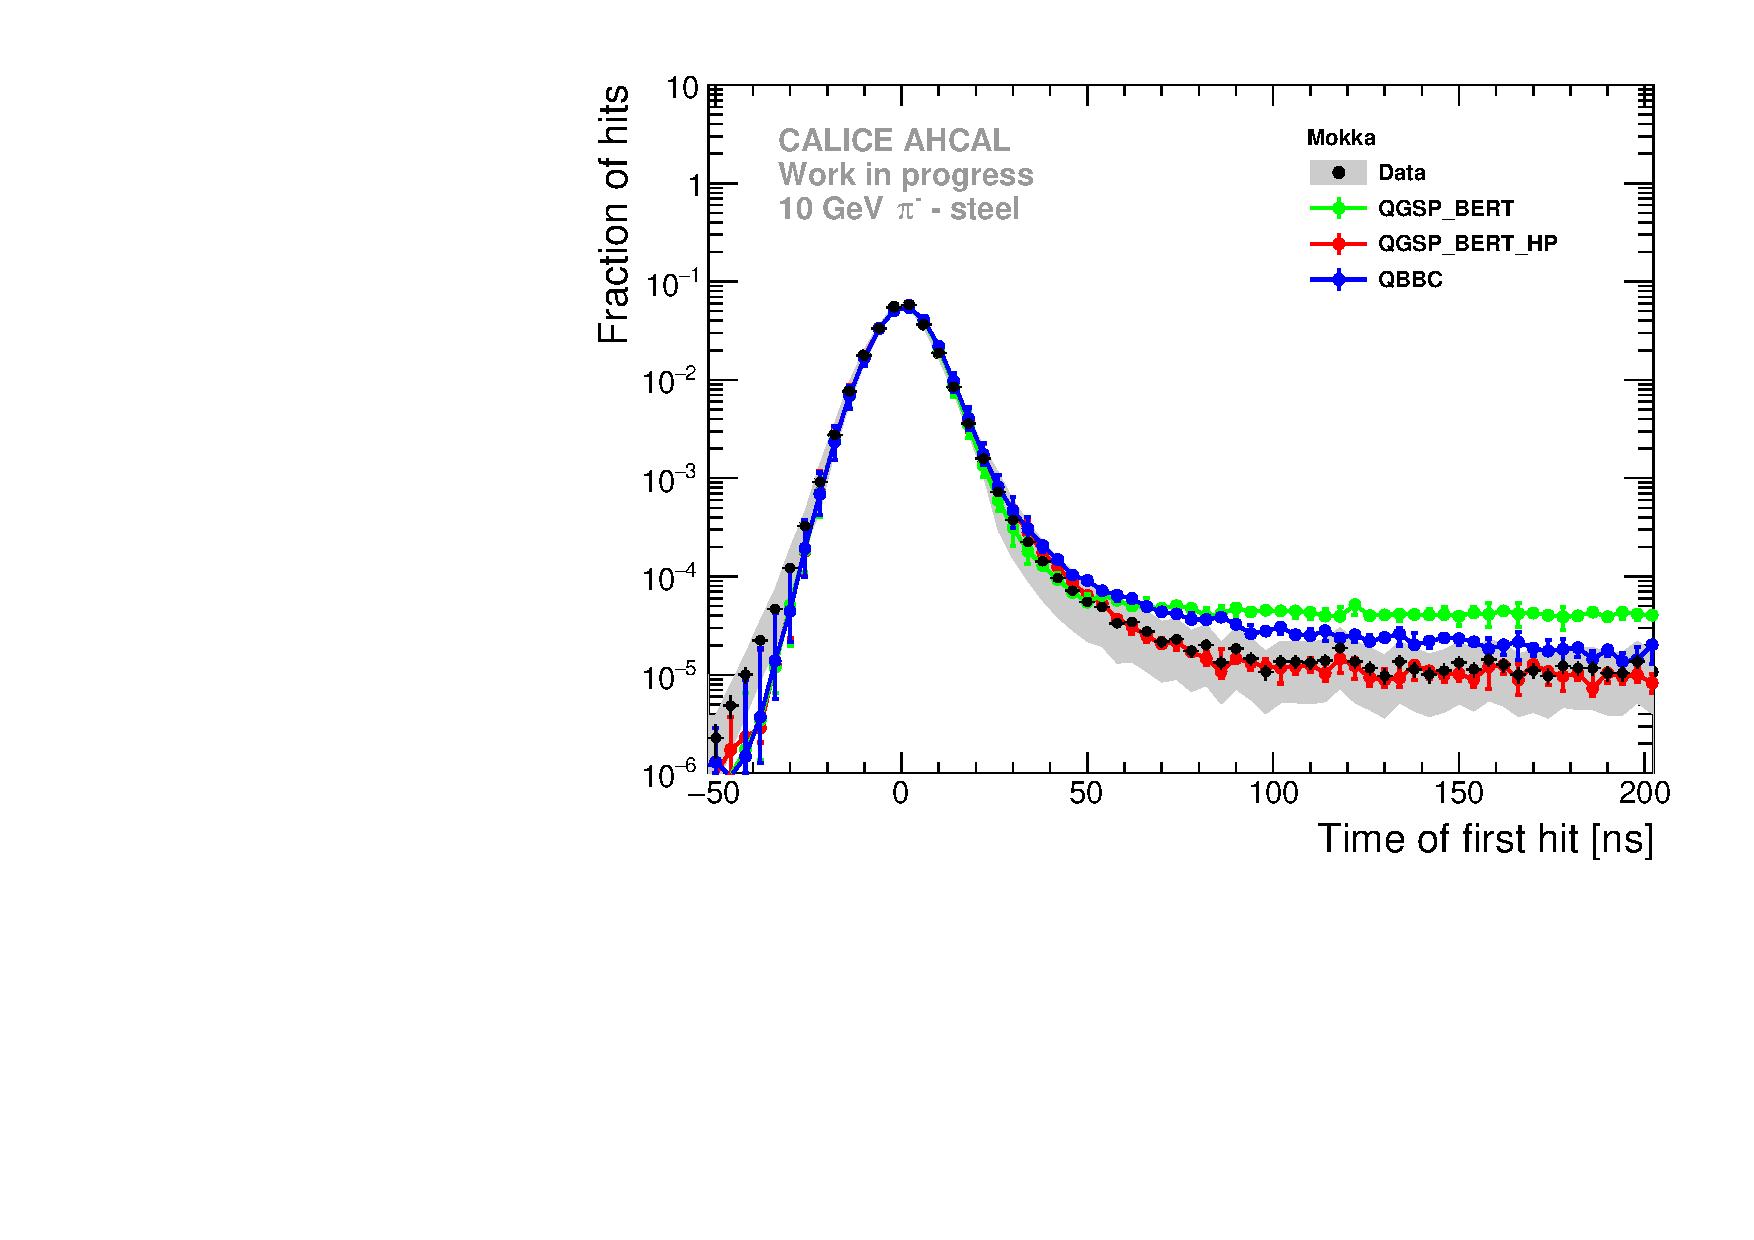
\includegraphics[width=1\textwidth]{chap5/fig_AHCAL_timing/Pions/Comparison_SimData_Pion10GeV_LateClusters.pdf}
		\caption{10 GeV.} \label{fig:dNdt_SimData_10GeV}
	\end{subfigure}
	\hfill
	\begin{subfigure}[t]{0.5\textwidth}
		\centering
		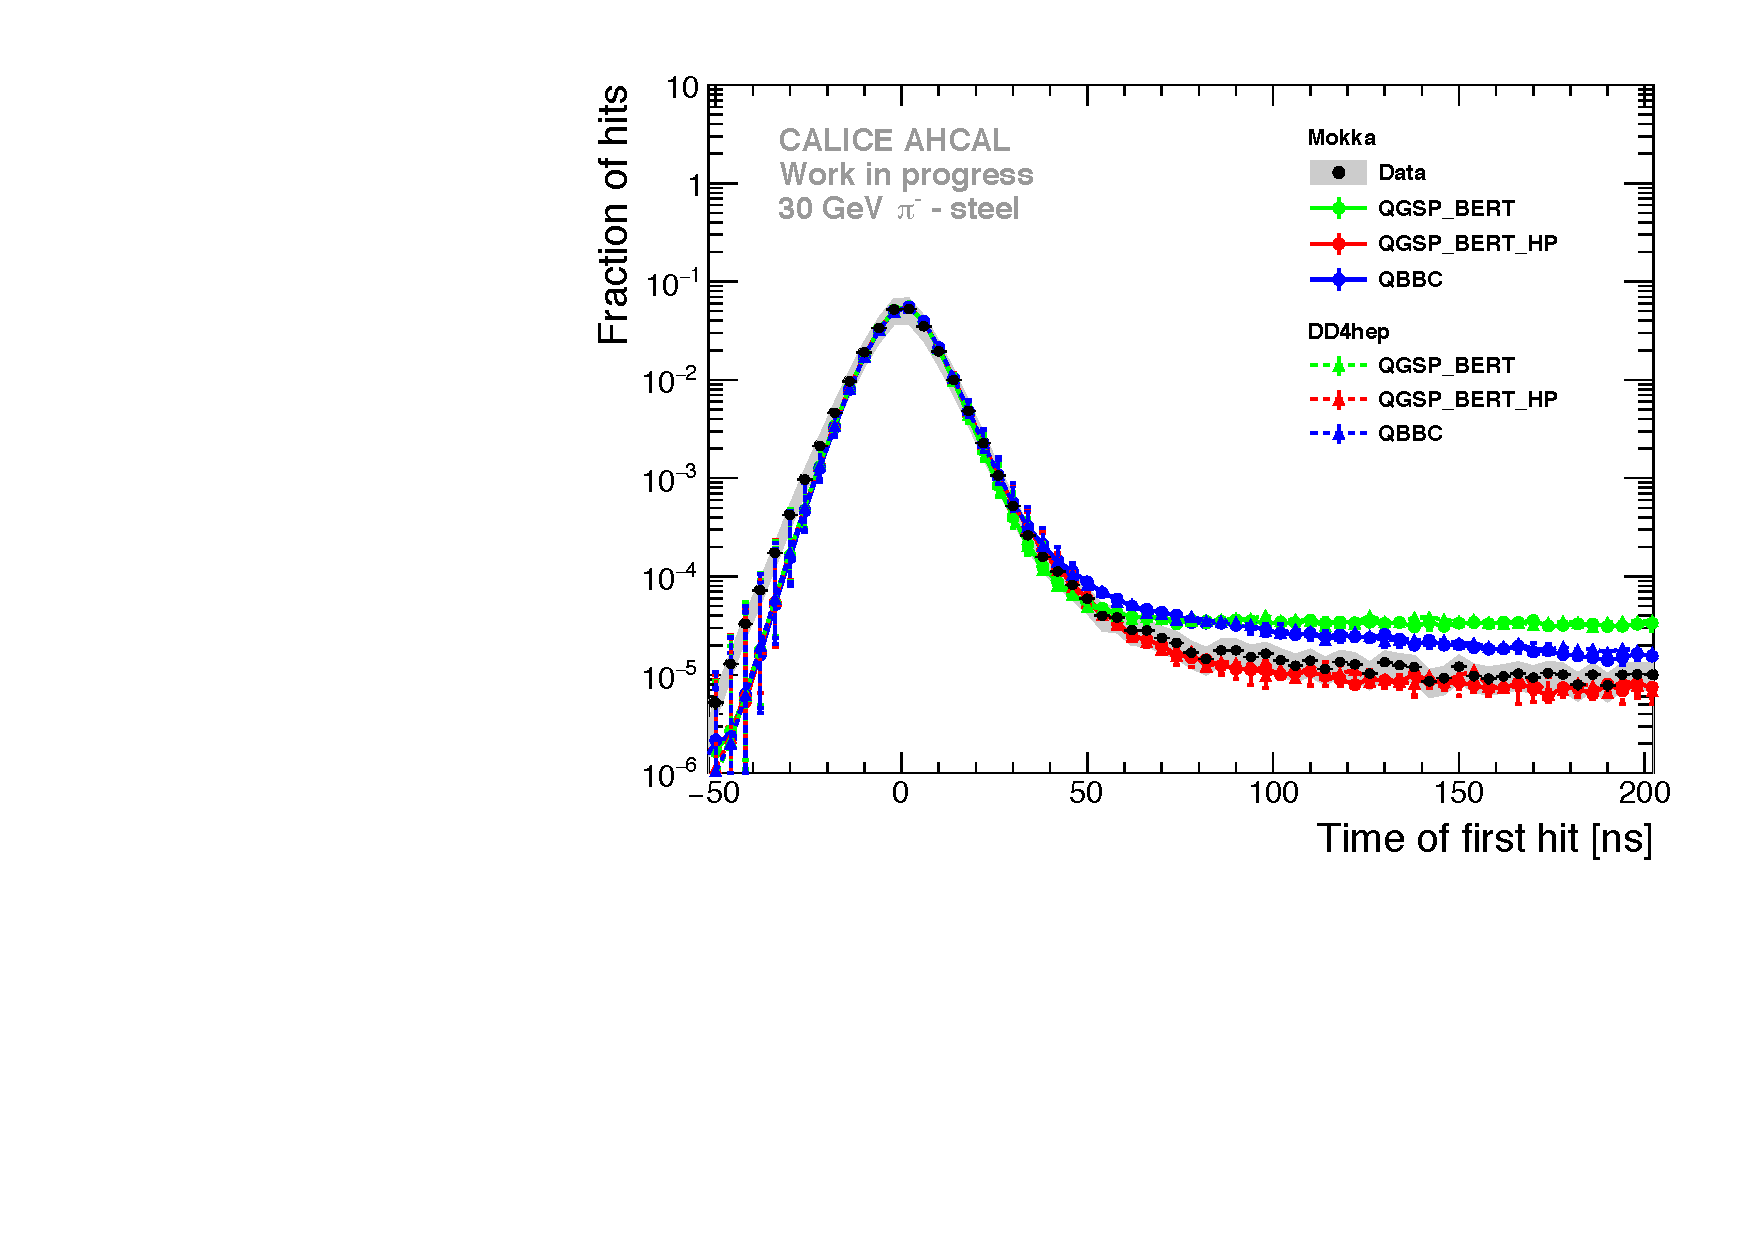
\includegraphics[width=1\textwidth]{chap5/fig_AHCAL_timing/Pions/Comparison_SimData_Pion30GeV_LateClusters.pdf}
		\caption{30 GeV.}\label{fig:dNdt_SimData_30GeV}
	\end{subfigure}
	\begin{subfigure}[t]{0.5\textwidth}
		\centering
		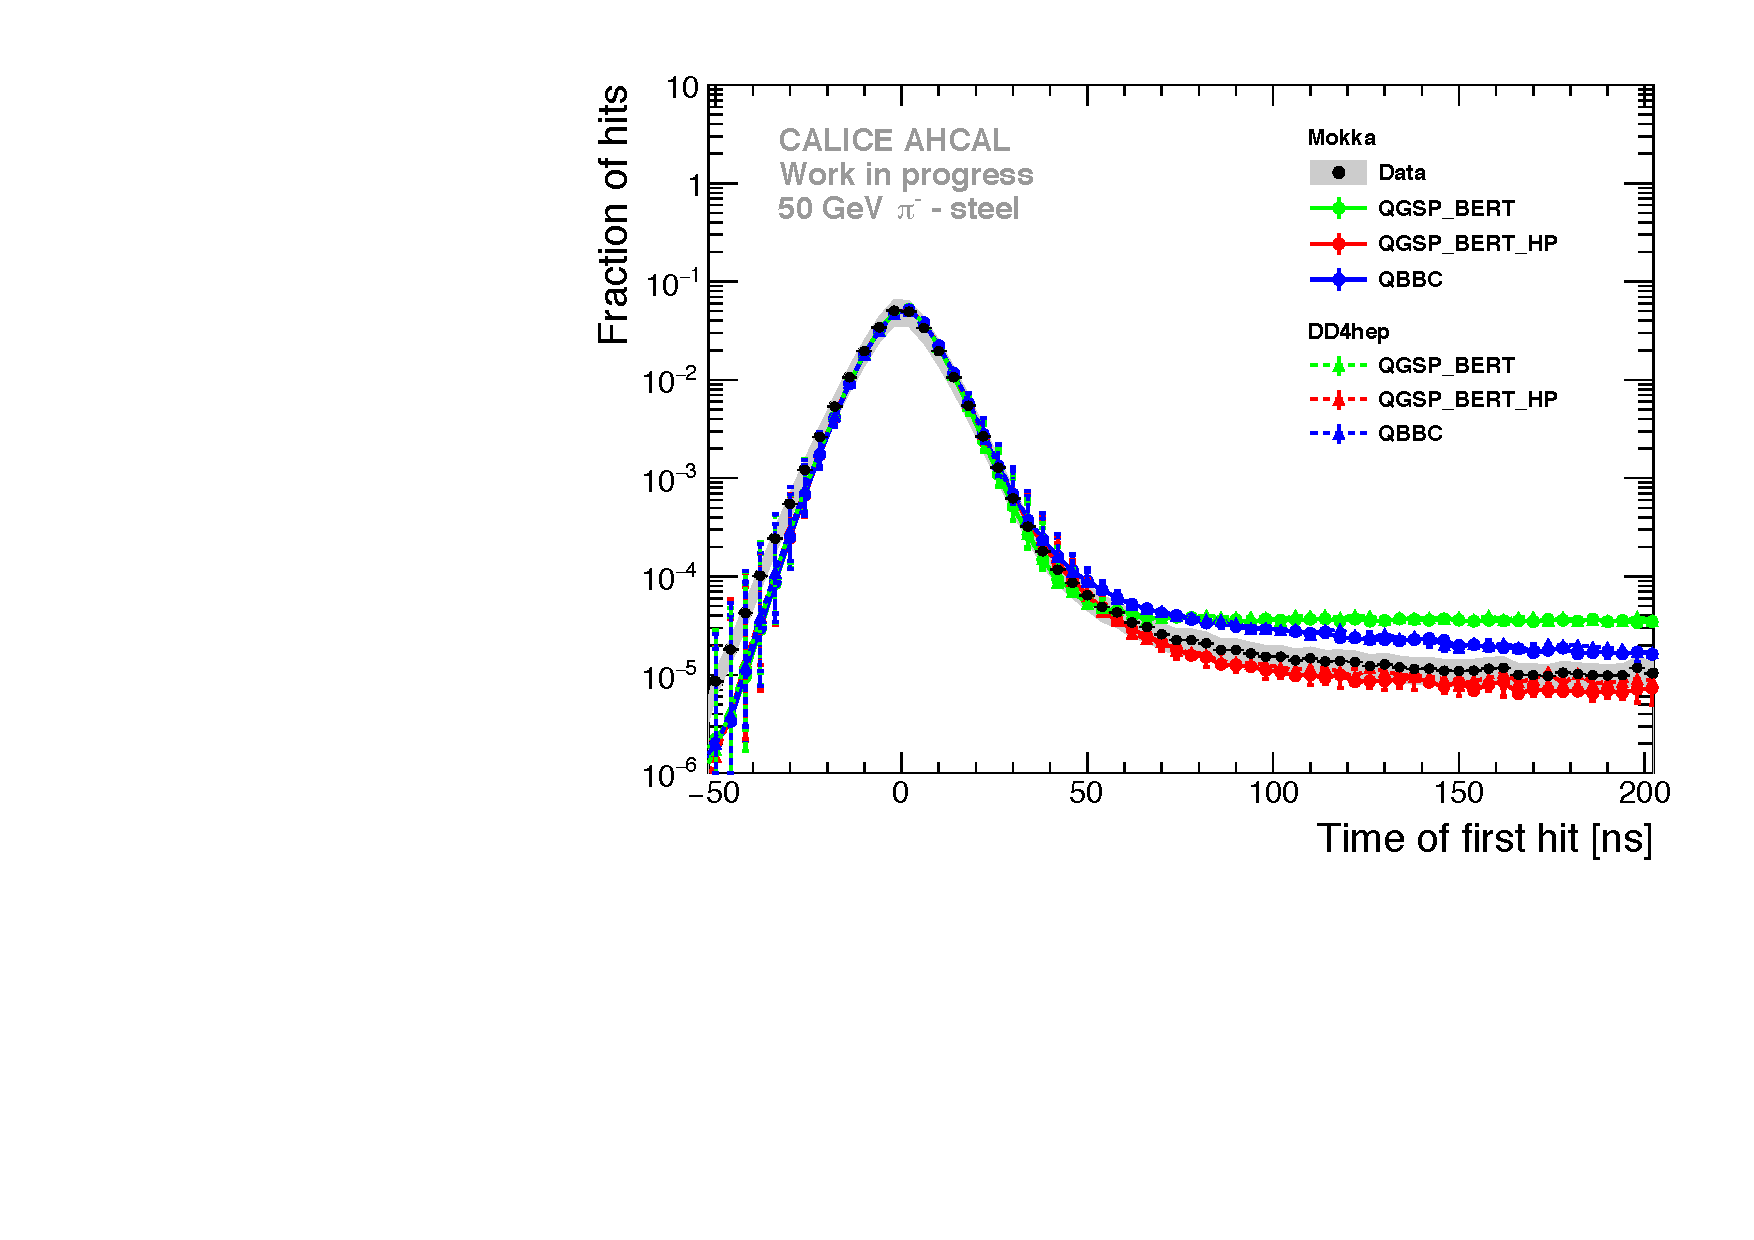
\includegraphics[width=1\textwidth]{chap5/fig_AHCAL_timing/Pions/Comparison_SimData_Pion50GeV_LateClusters.pdf}
		\caption{50 GeV.} \label{fig:dNdt_SimData_50GeV}
	\end{subfigure}
	\hfill
	\begin{subfigure}[t]{0.5\textwidth}
		\centering
		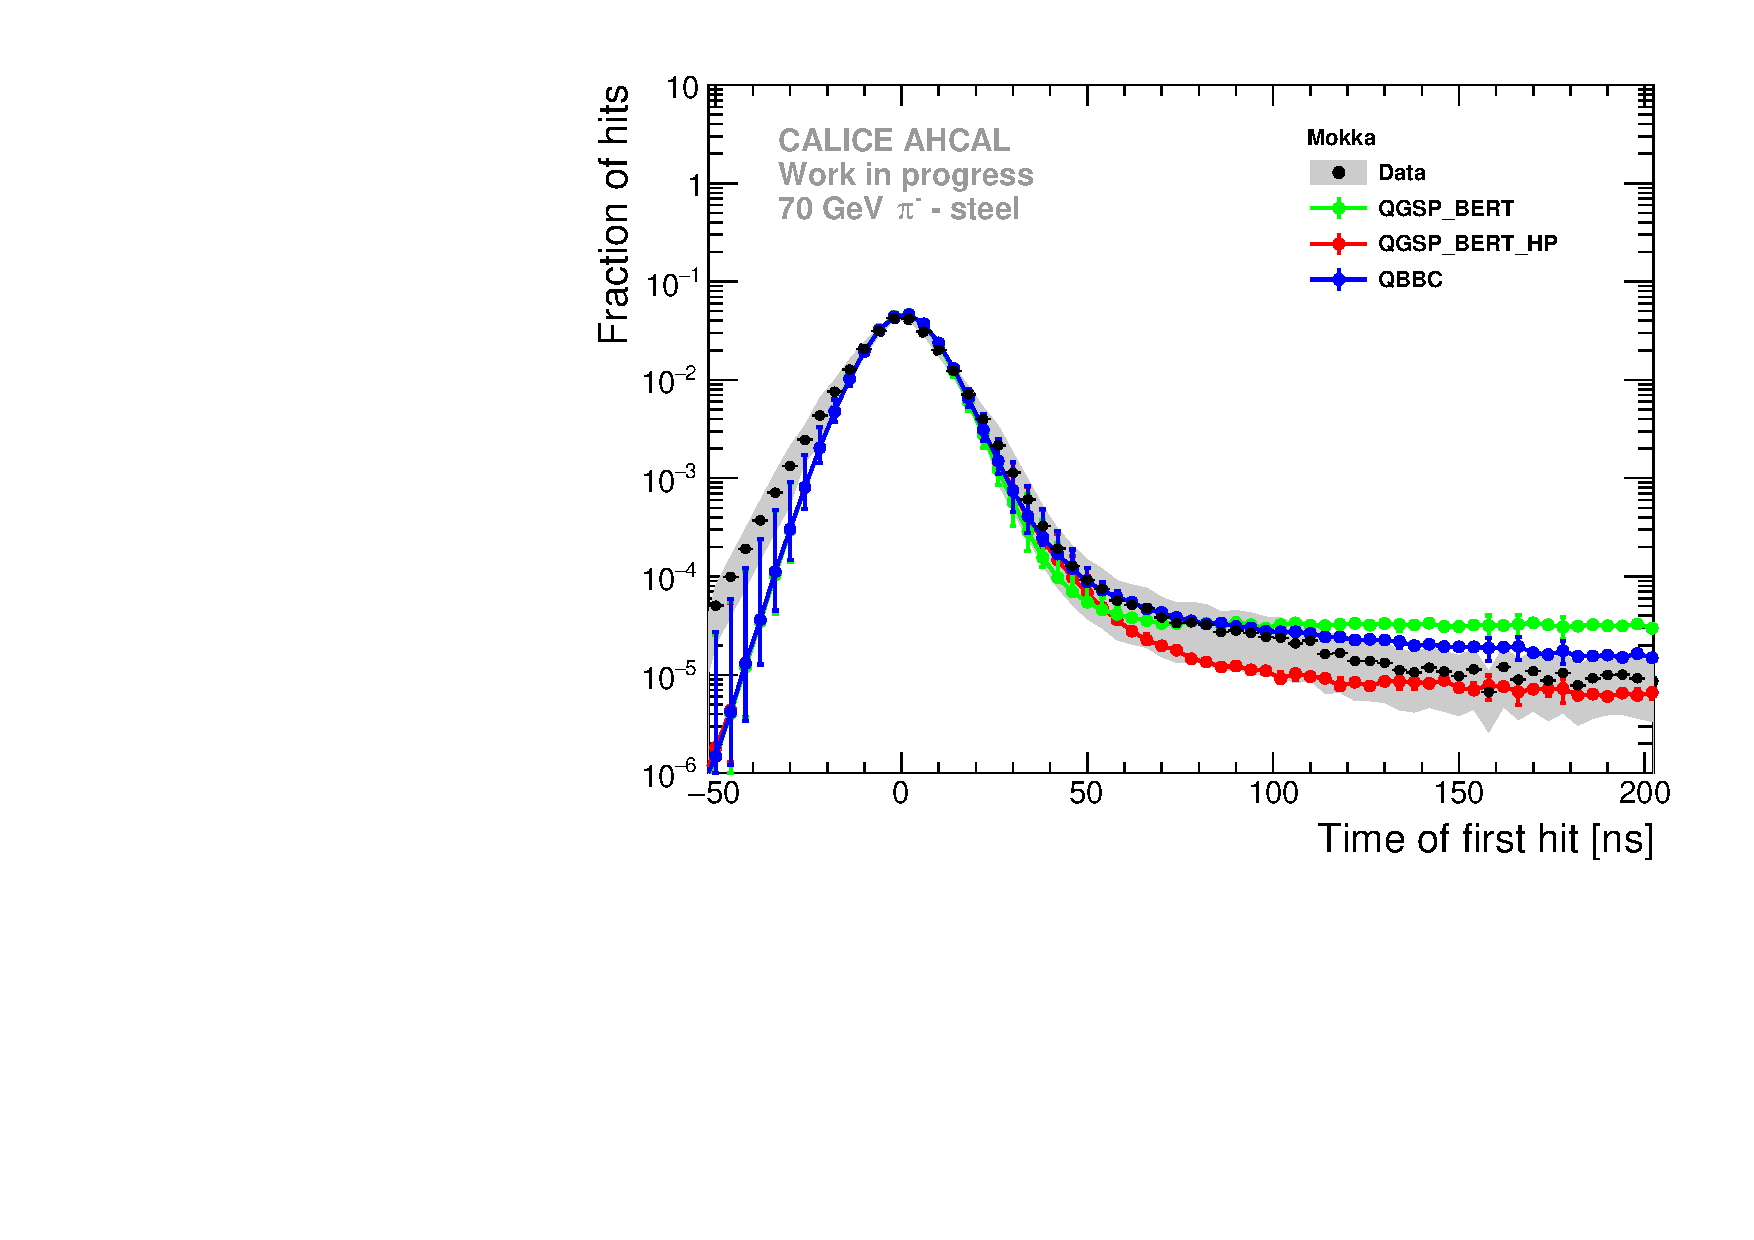
\includegraphics[width=1\textwidth]{chap5/fig_AHCAL_timing/Pions/Comparison_SimData_Pion70GeV_LateClusters.pdf}
		\caption{70 GeV.} \label{fig:dNdt_SimData_70GeV}
	\end{subfigure}
	\hfill
	\begin{subfigure}[t]{0.5\textwidth}
		\centering
		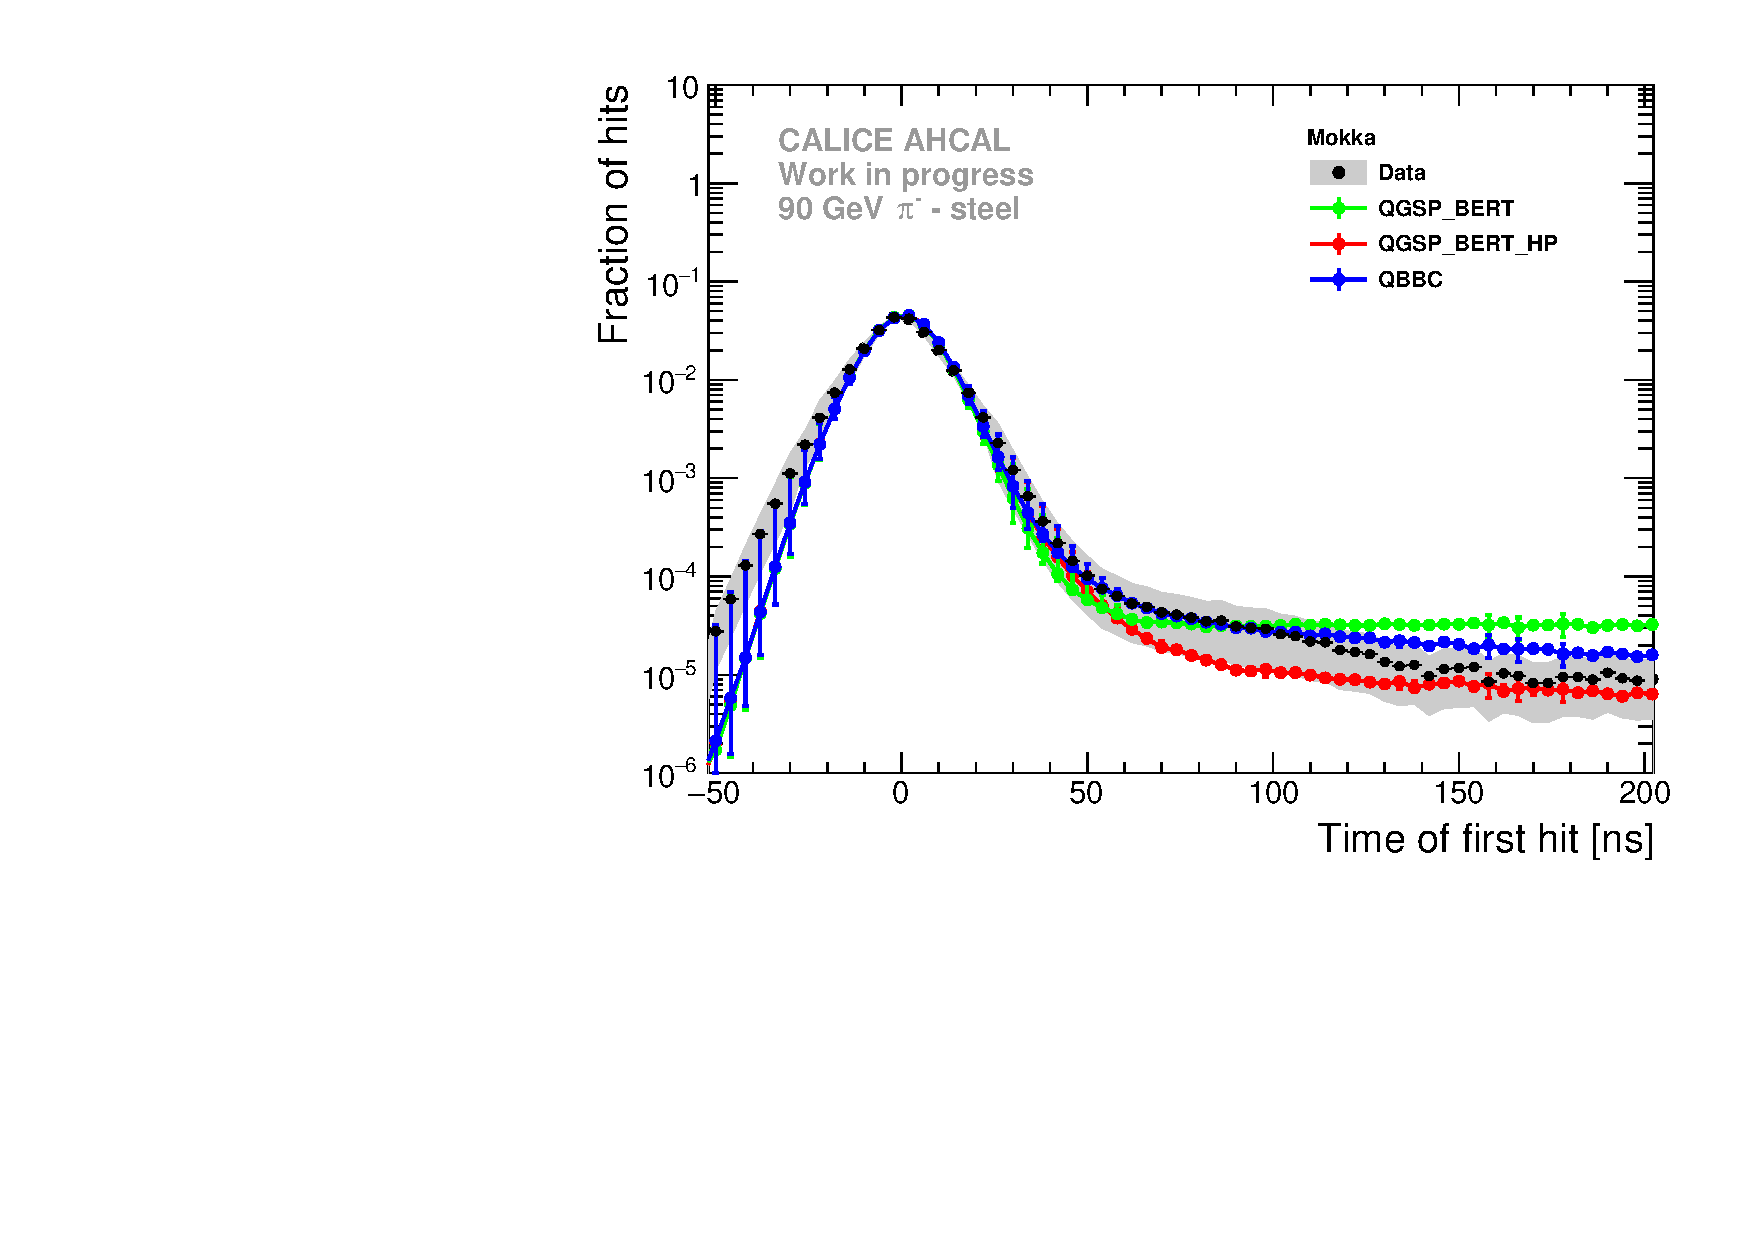
\includegraphics[width=1\textwidth]{chap5/fig_AHCAL_timing/Pions/Comparison_SimData_Pion90GeV_LateClusters.pdf}
		\caption{90 GeV.} \label{fig:dNdt_SimData_90GeV}
	\end{subfigure}
	\caption{Comparison between simulations and data of the time of first hit per bin time for pion beams between 10 GeV and 90 GeV. The grey and color bands shows the systematics.}
	\label{fig:dNdt_SimData_Comparison}
\end{figure}

\begin{figure}[htbp!]
	\begin{subfigure}[t]{0.5\textwidth}
		\centering
		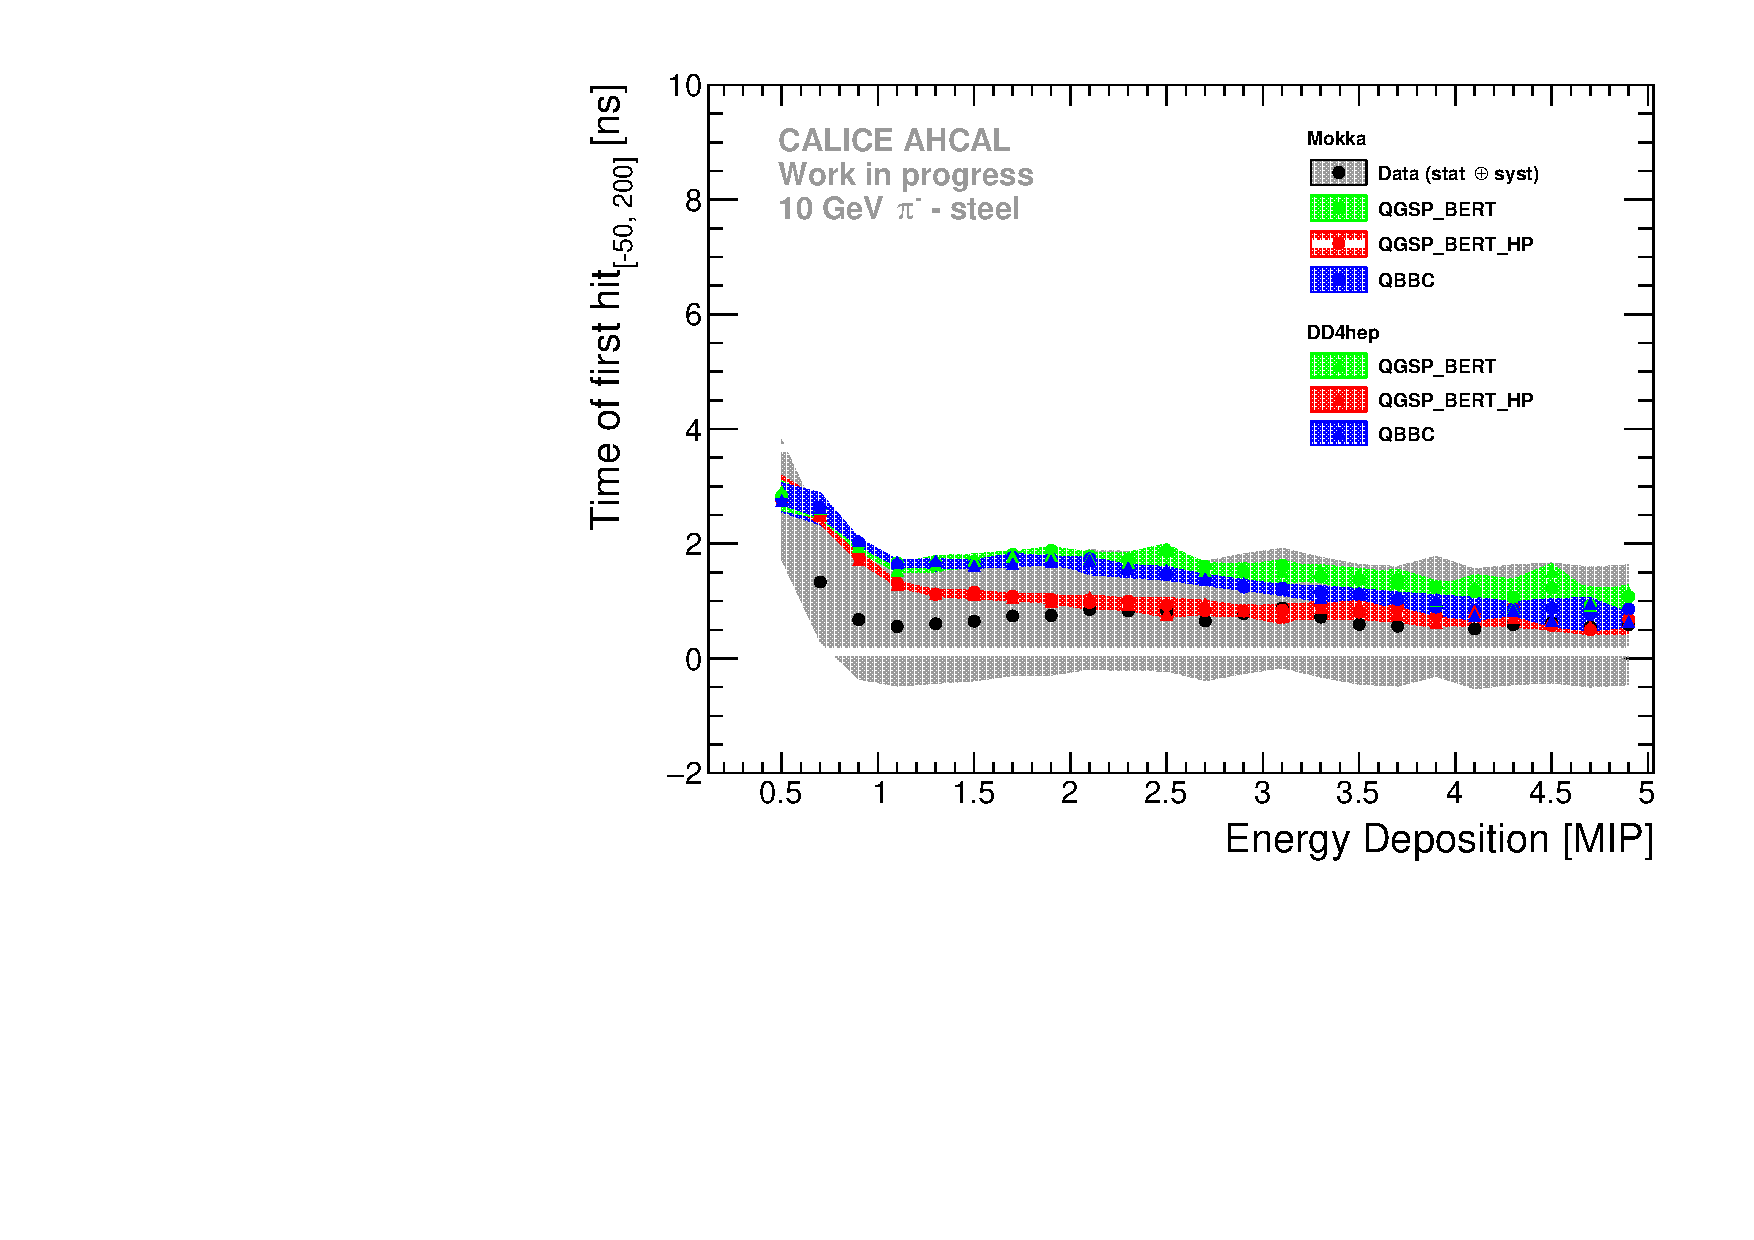
\includegraphics[width=1\textwidth]{chap5/fig_AHCAL_timing/Pions/ComparisonToSim/Time_Energy_10GeV.pdf}
		\caption{10 GeV.} \label{fig:Energy_SimData_10GeV}
	\end{subfigure}
	\hfill
	\begin{subfigure}[t]{0.5\textwidth}
		\centering
		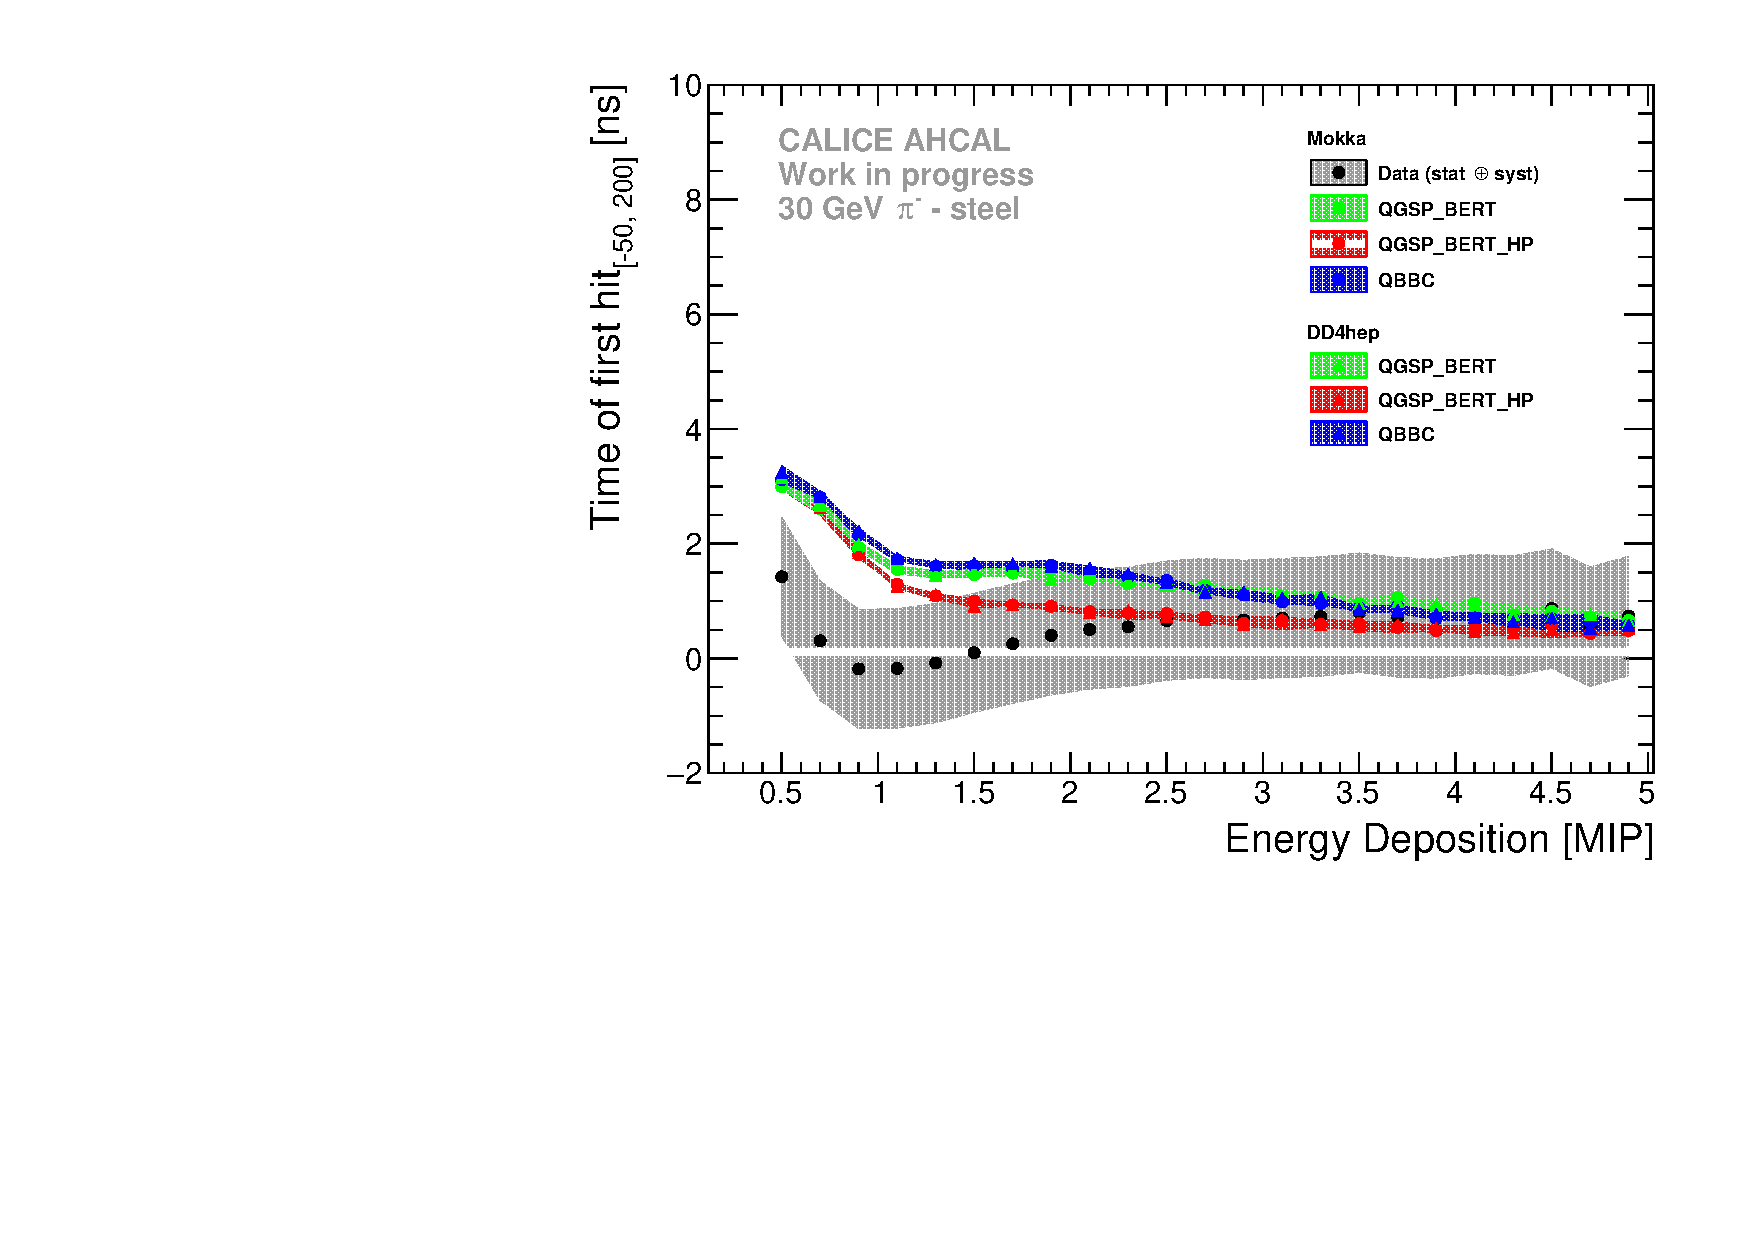
\includegraphics[width=1\textwidth]{chap5/fig_AHCAL_timing/Pions/ComparisonToSim/Time_Energy_30GeV.pdf}
		\caption{30 GeV.}\label{fig:Energy_SimData_30GeV}
	\end{subfigure}
	\begin{subfigure}[t]{0.5\textwidth}
		\centering
		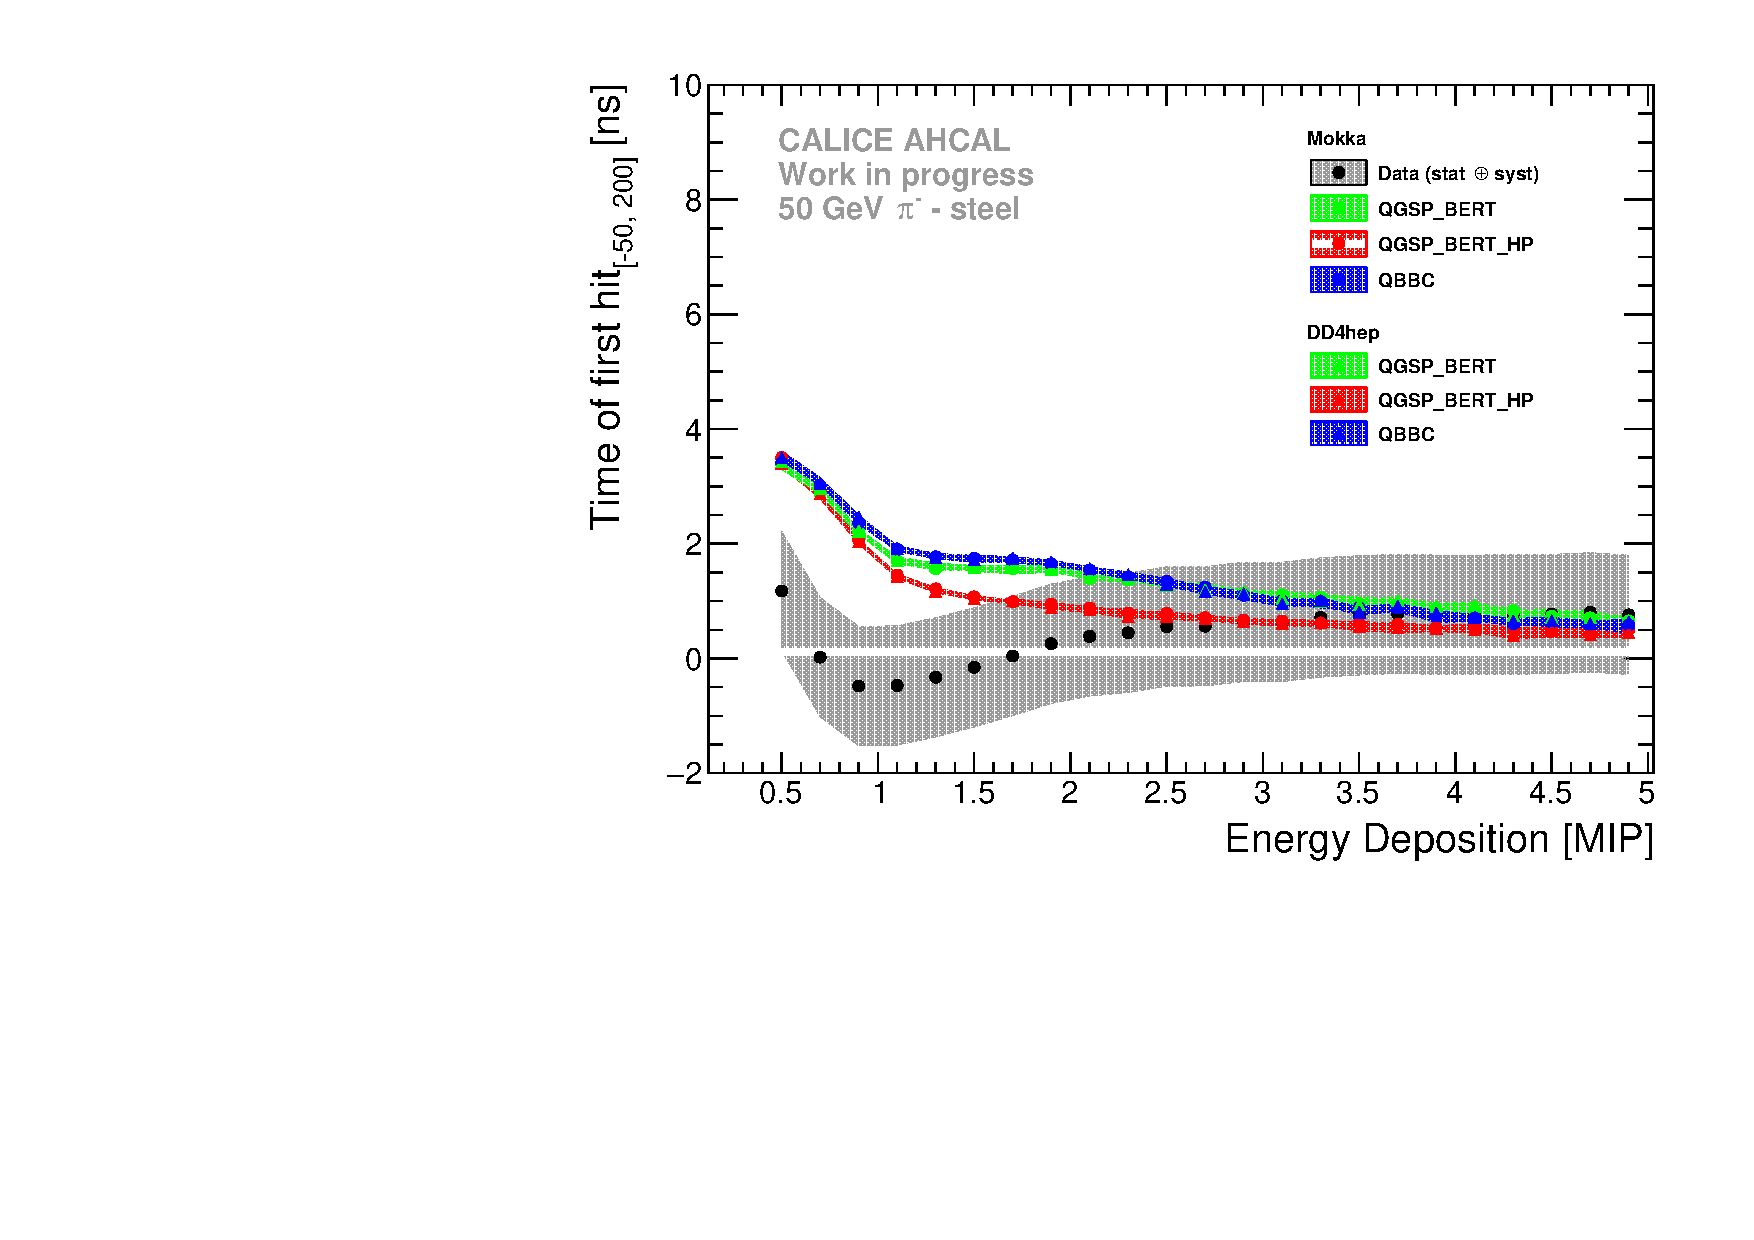
\includegraphics[width=1\textwidth]{chap5/fig_AHCAL_timing/Pions/ComparisonToSim/Time_Energy_50GeV.pdf}
		\caption{50 GeV.} \label{fig:Energy_SimData_50GeV}
	\end{subfigure}
	\hfill
	\begin{subfigure}[t]{0.5\textwidth}
		\centering
		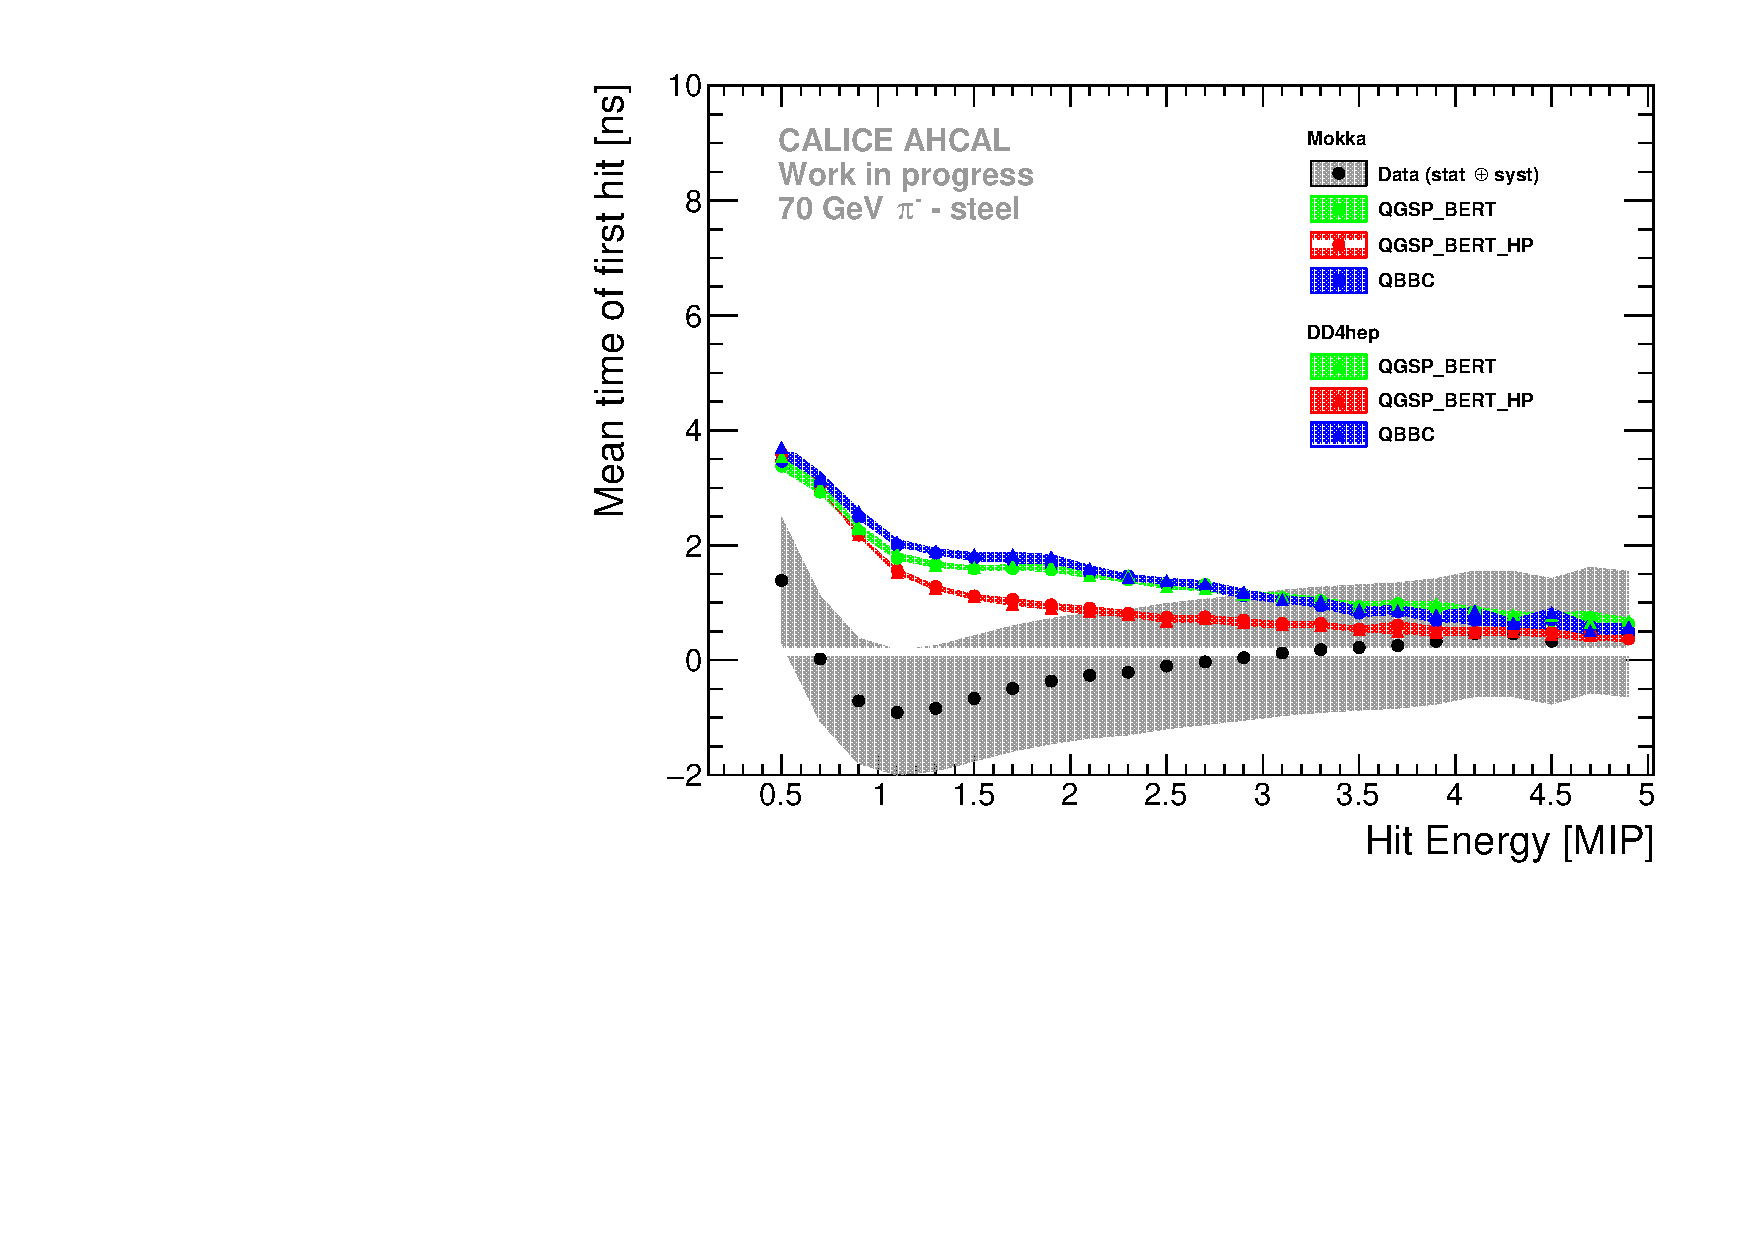
\includegraphics[width=1\textwidth]{chap5/fig_AHCAL_timing/Pions/ComparisonToSim/Time_Energy_70GeV.pdf}
		\caption{70 GeV.} \label{fig:Energy_SimData_70GeV}
	\end{subfigure}
	\hfill
	\begin{subfigure}[t]{0.5\textwidth}
		\centering
		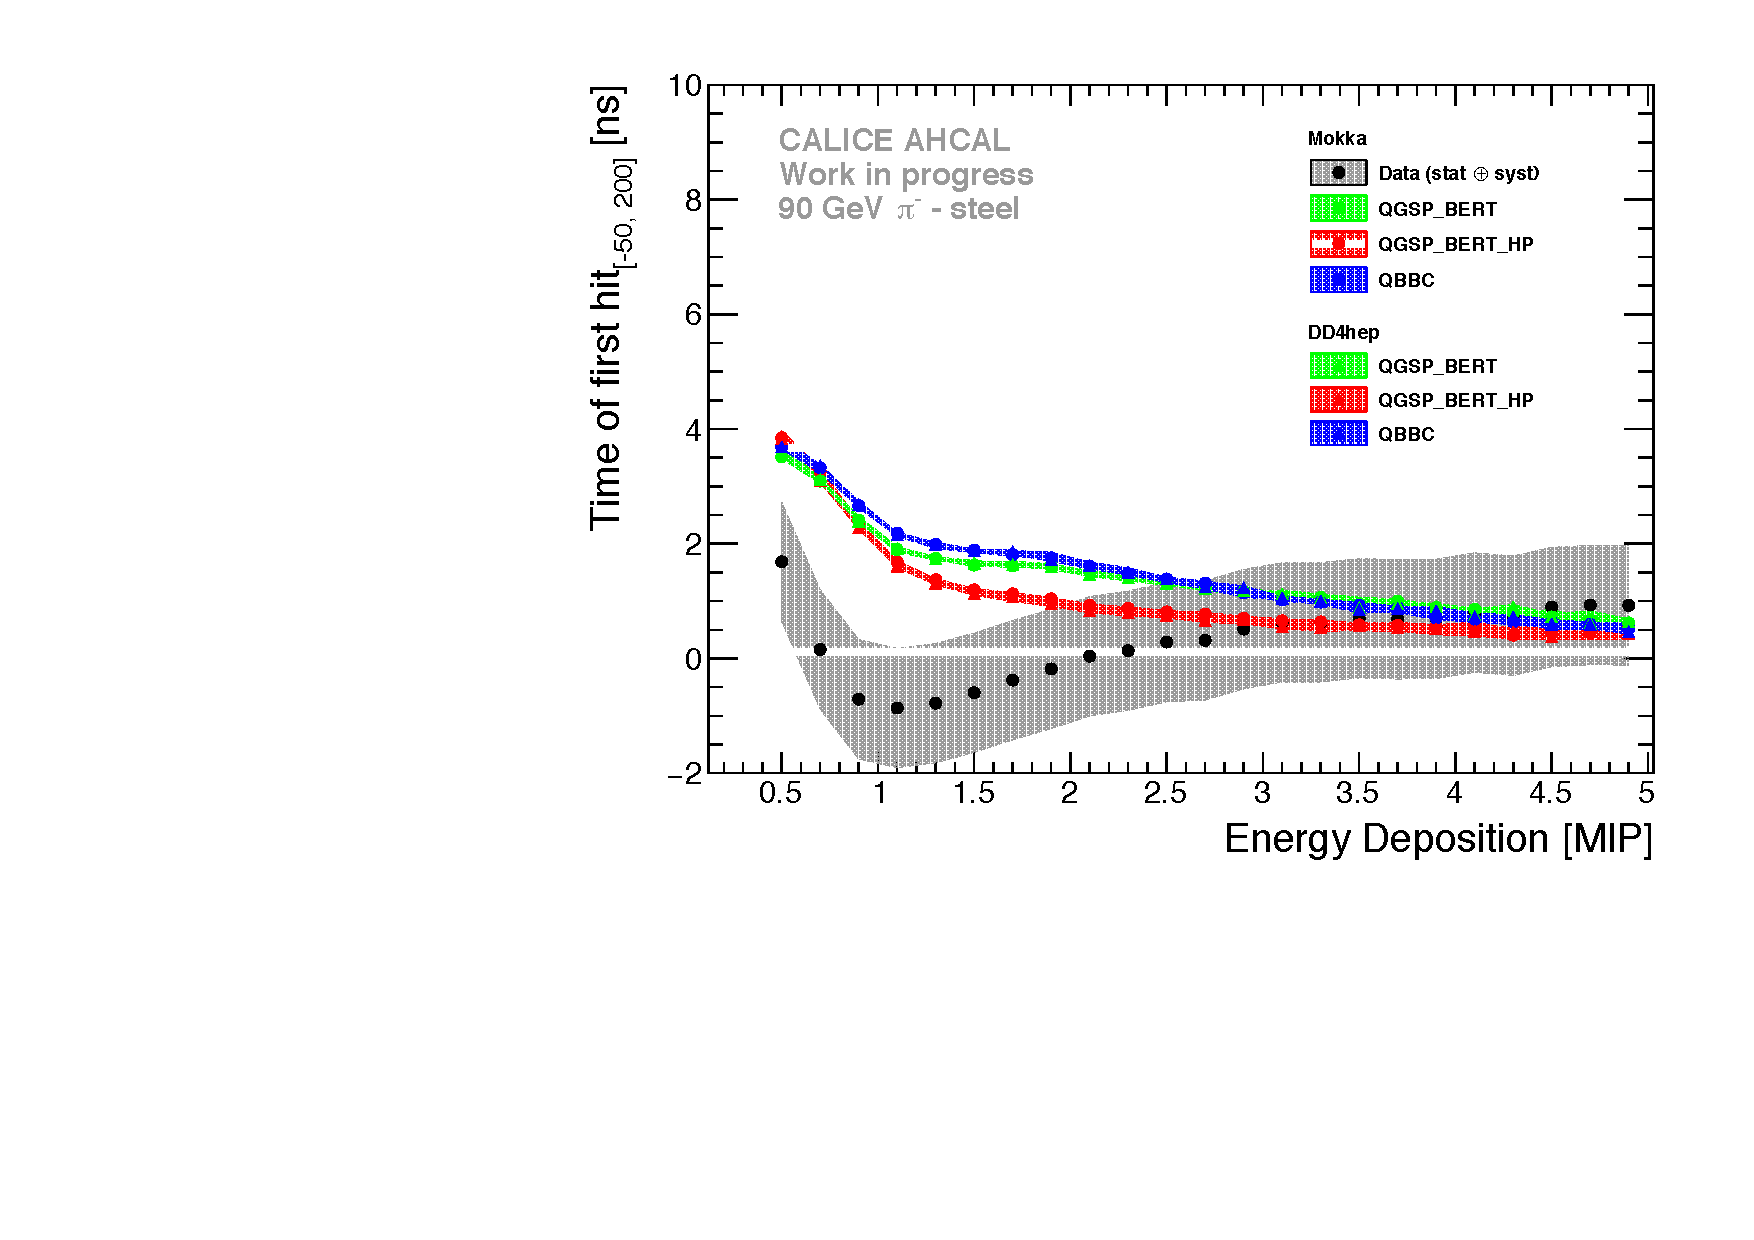
\includegraphics[width=1\textwidth]{chap5/fig_AHCAL_timing/Pions/ComparisonToSim/Time_Energy_90GeV.pdf}
		\caption{90 GeV.} \label{fig:Energy_SimData_90GeV}
	\end{subfigure}
	\caption{Comparison between simulations and data of the time of first hit as function of the hit energy for pion beams between 10 GeV and 90 GeV. The grey and color bands shows the systematics.}
	\label{fig:Energy_SimData_Comparison}
\end{figure}

\begin{figure}[htbp!]
	\begin{subfigure}[t]{0.5\textwidth}
		\centering
		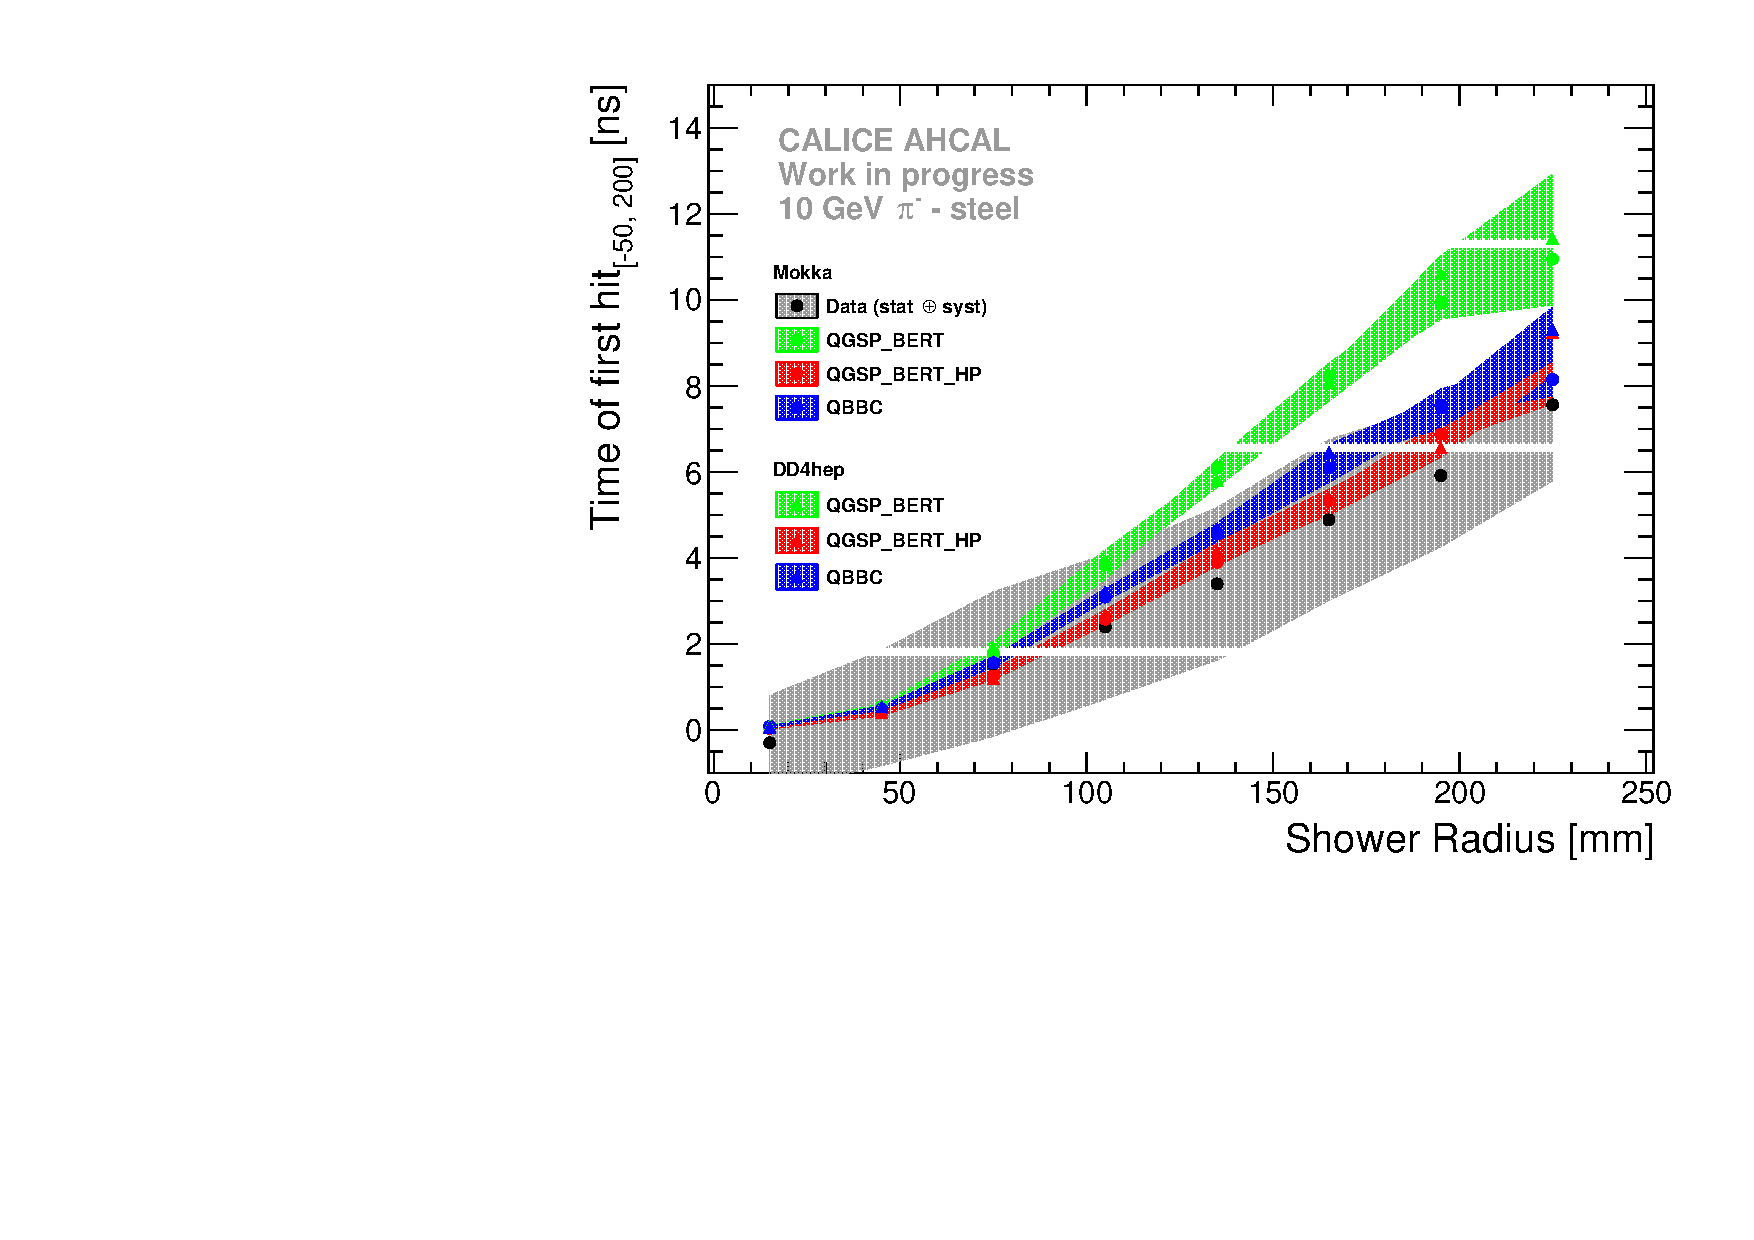
\includegraphics[width=1\textwidth]{chap5/fig_AHCAL_timing/Pions/ComparisonToSim/Time_Radius_10GeV_SSF.pdf}
		\caption{10 GeV (SSF).} \label{fig:Radius_SSF_SimData_10GeV}
	\end{subfigure}
	\hfill
	\begin{subfigure}[t]{0.5\textwidth}
		\centering
		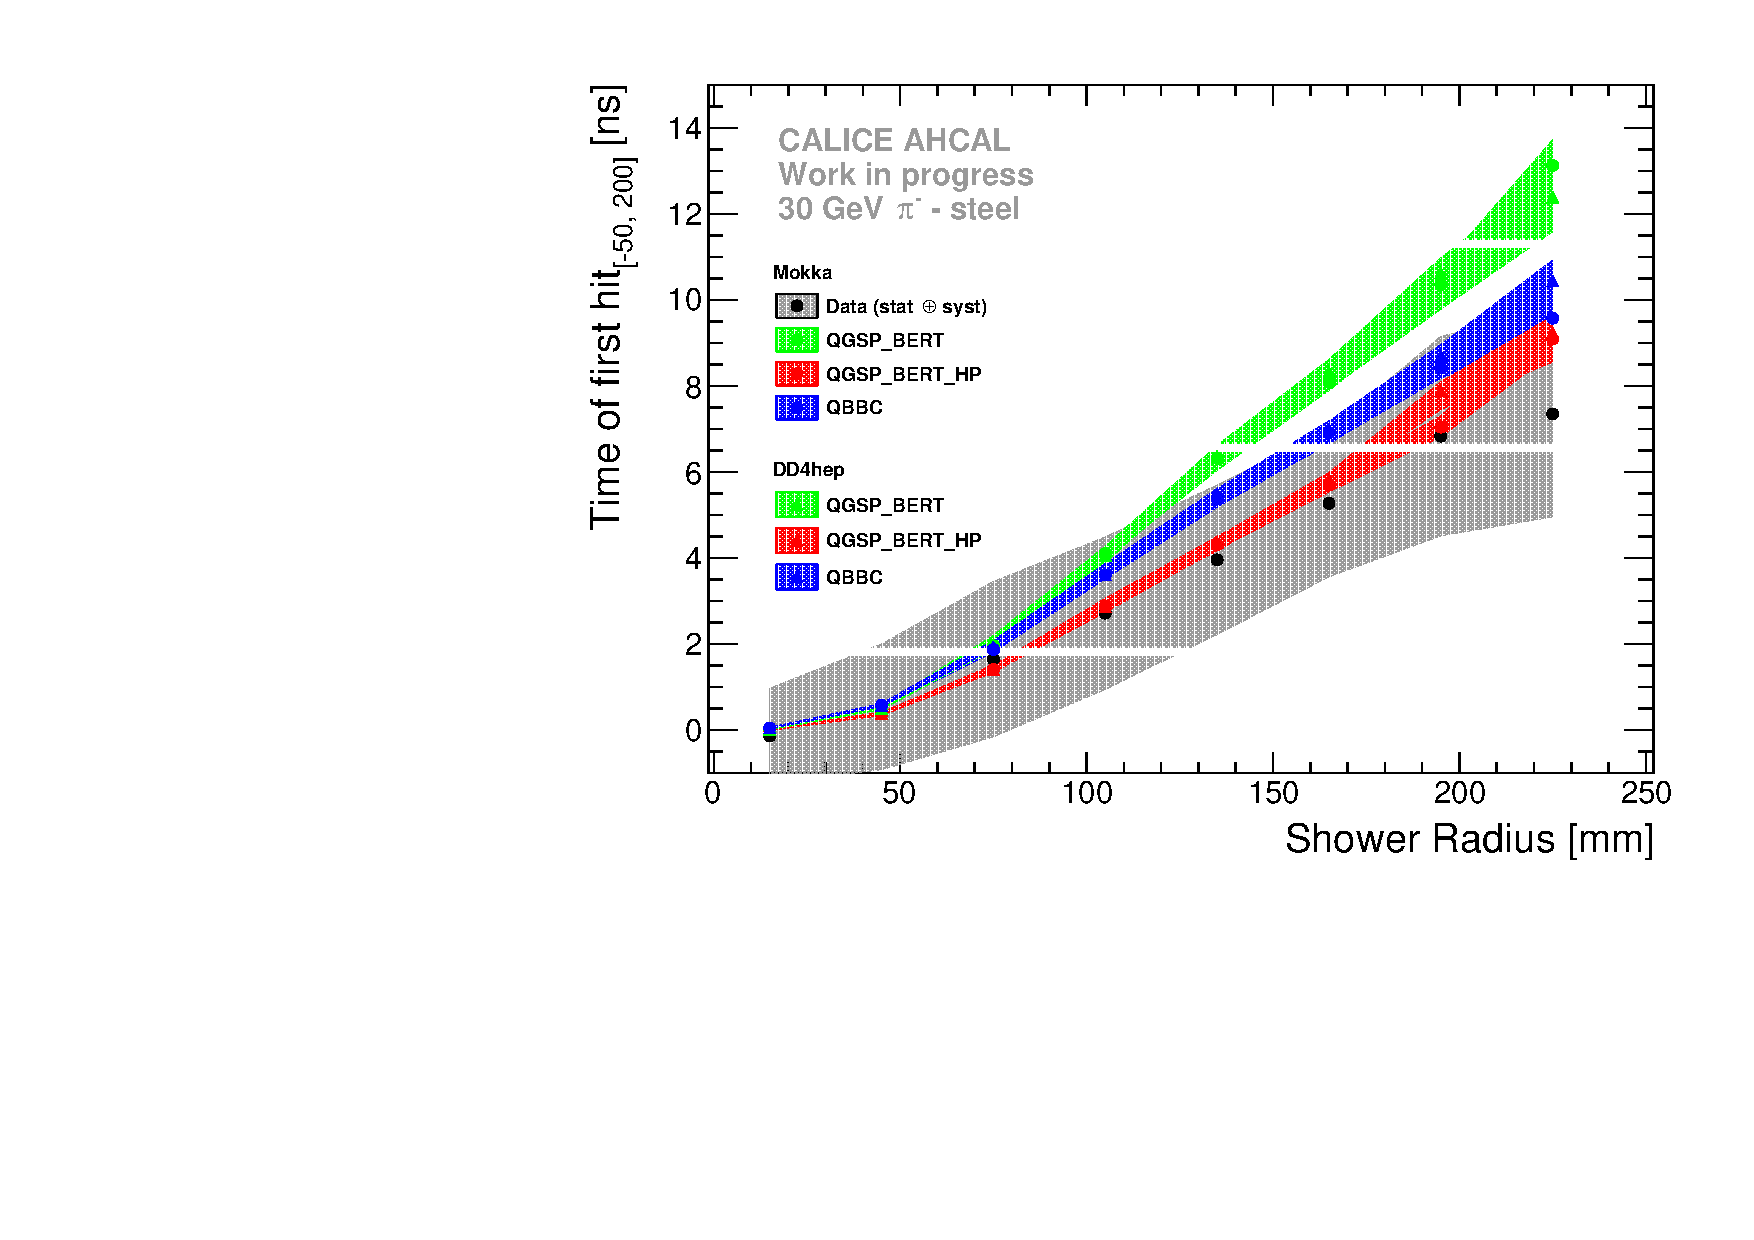
\includegraphics[width=1\textwidth]{chap5/fig_AHCAL_timing/Pions/ComparisonToSim/Time_Radius_30GeV_SSF.pdf}
		\caption{30 GeV (SSF).} \label{fig:Radius_SSF_SimData_30GeV}
	\end{subfigure}
	\hfill
	\begin{subfigure}[t]{0.5\textwidth}
		\centering
		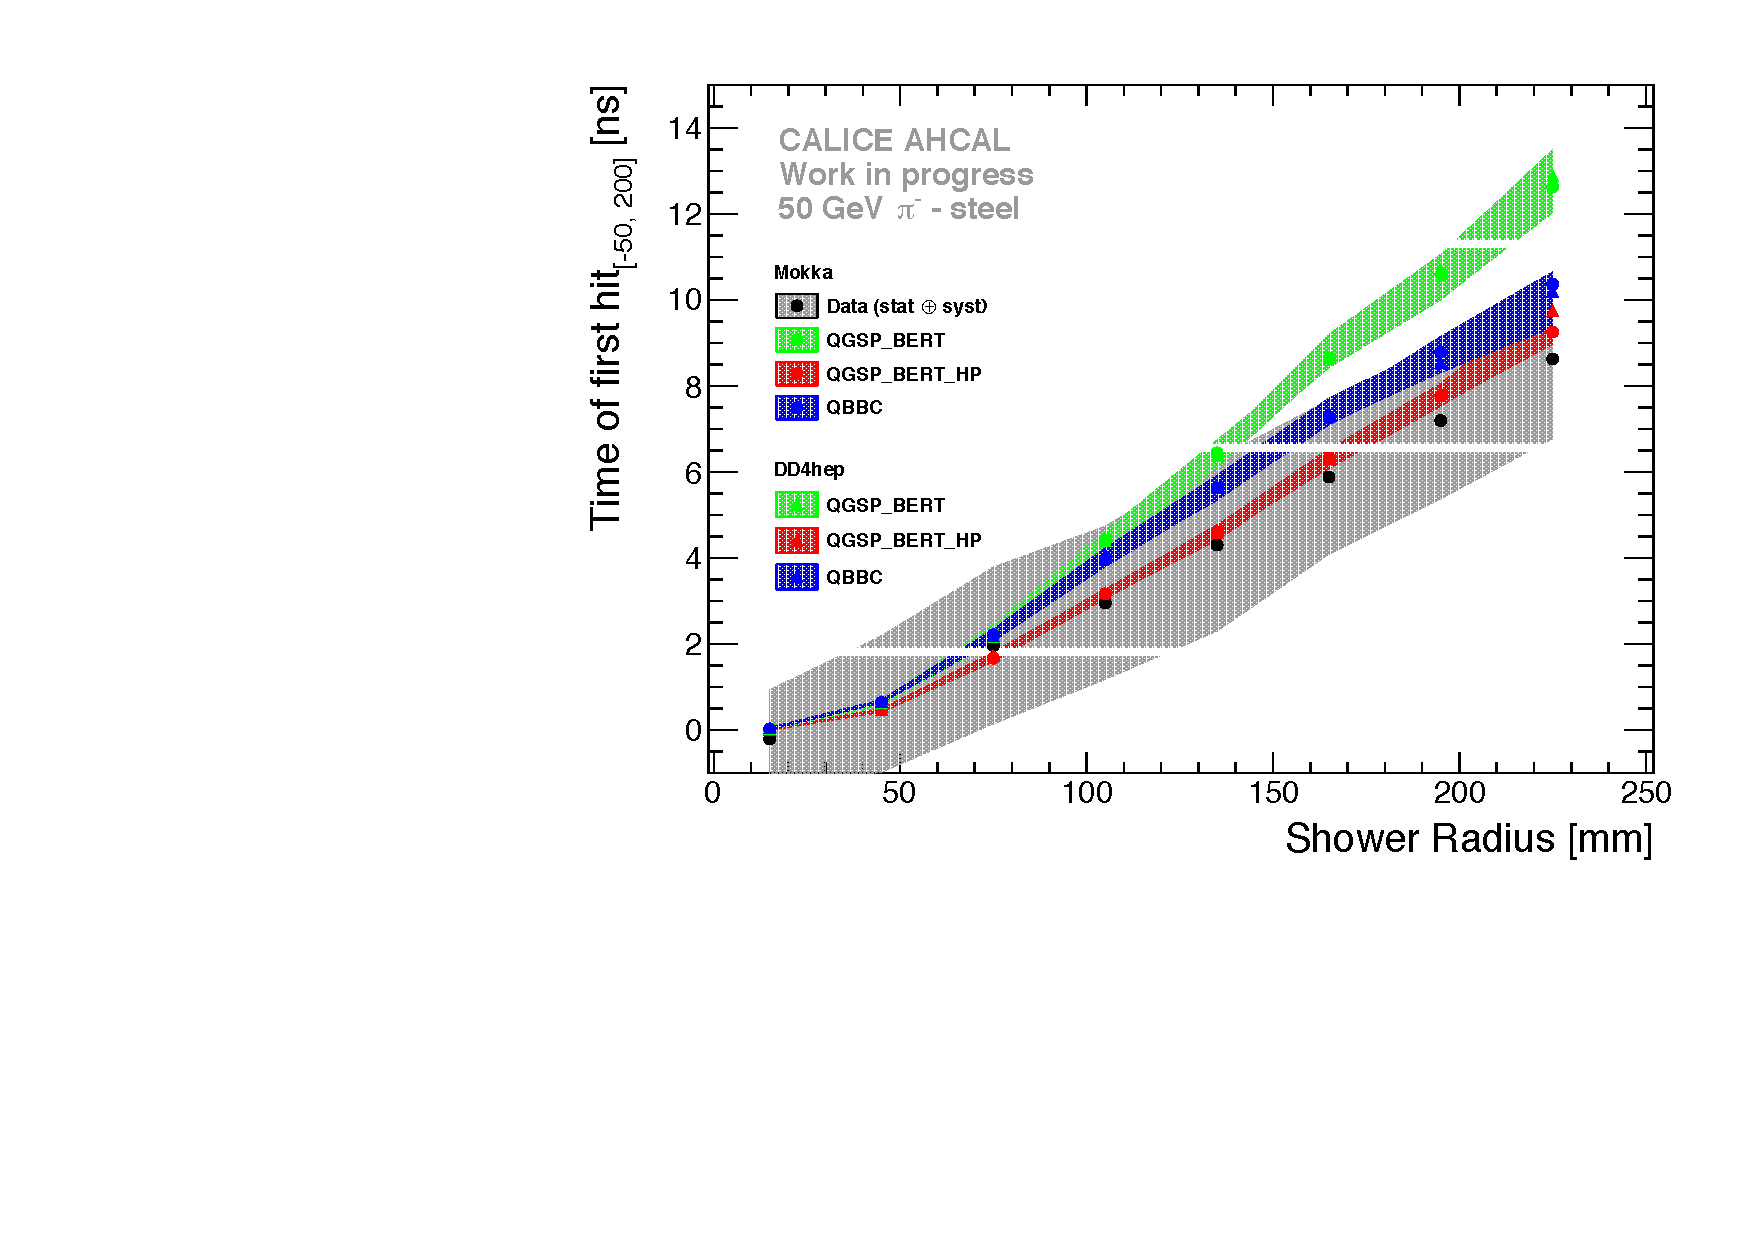
\includegraphics[width=1\textwidth]{chap5/fig_AHCAL_timing/Pions/ComparisonToSim/Time_Radius_50GeV_SSF.pdf}
		\caption{50 GeV (SSF).} \label{fig:Radius_SSF_SimData_50GeV}
	\end{subfigure}
	\hfill
	\begin{subfigure}[t]{0.5\textwidth}
		\centering
		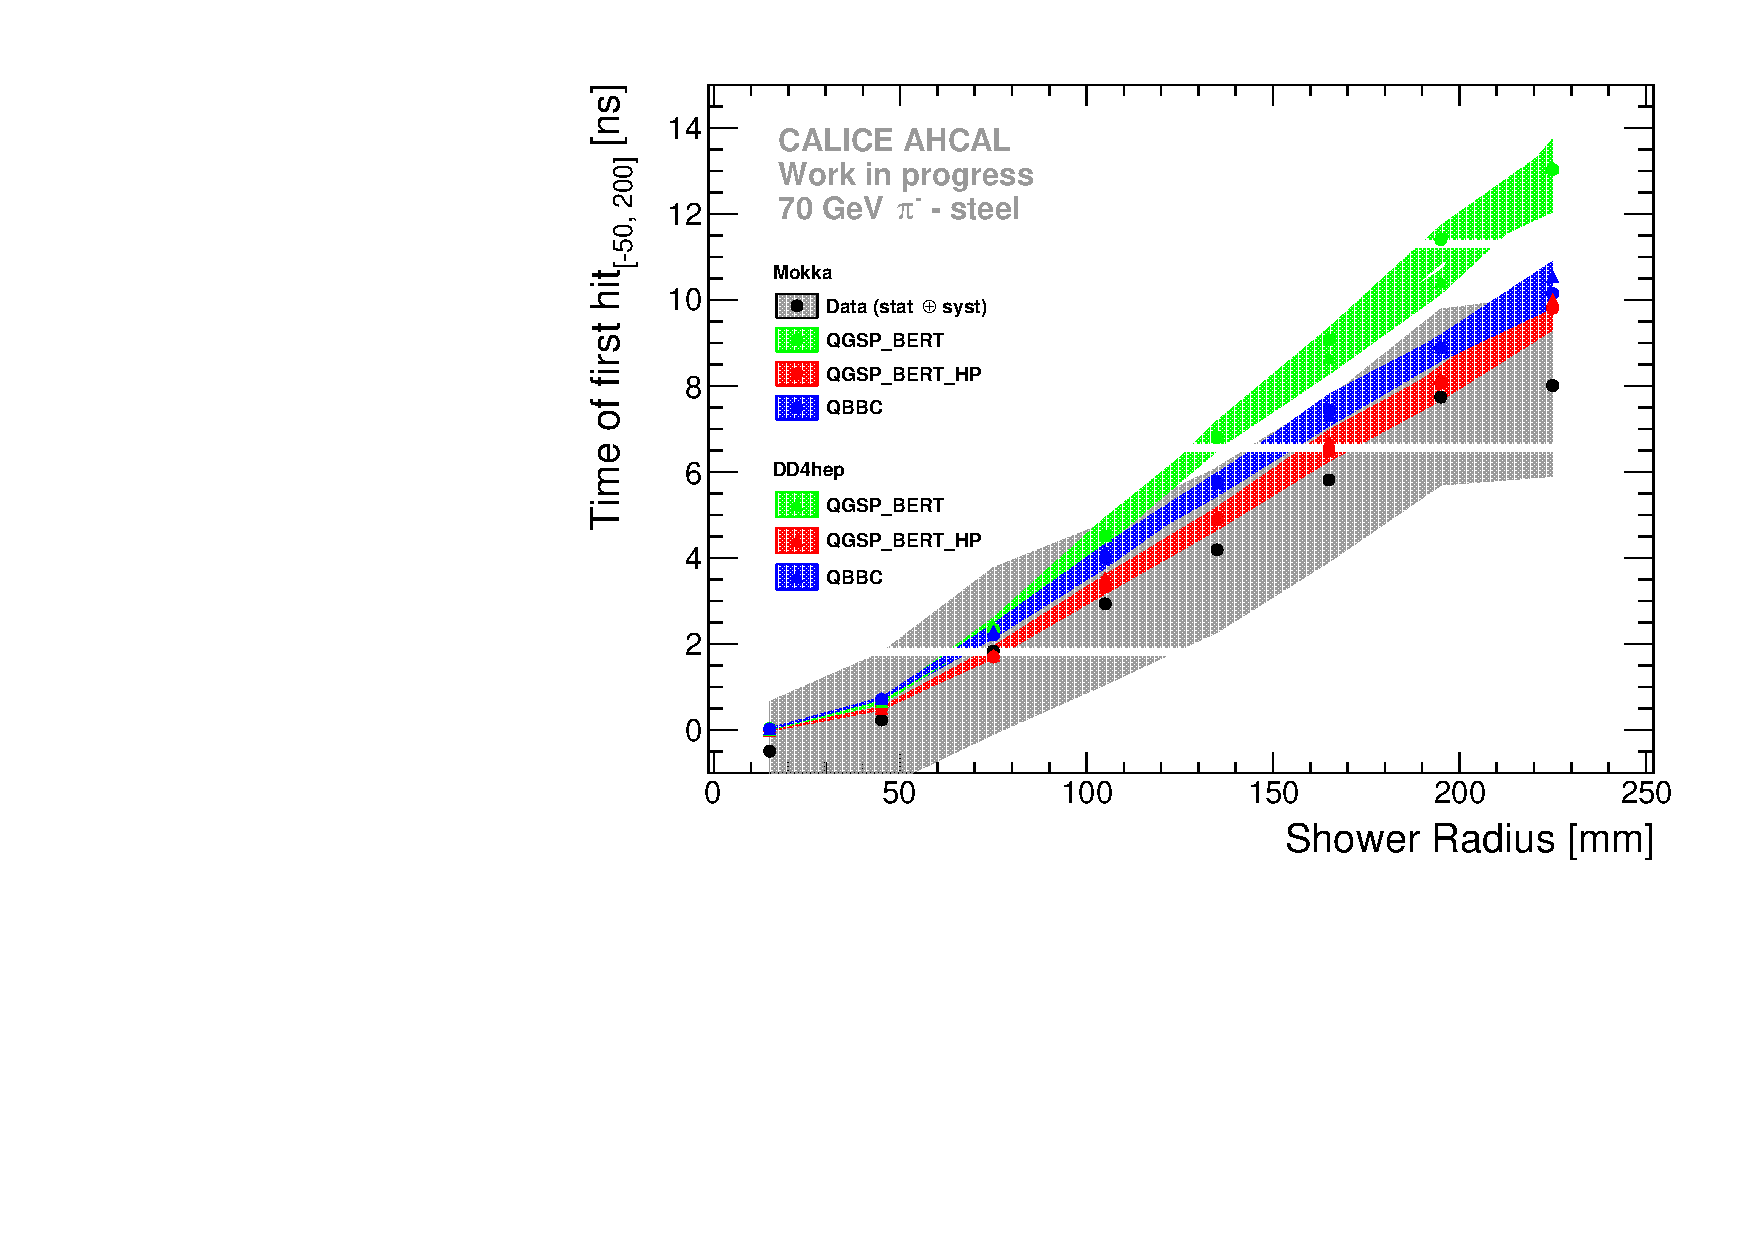
\includegraphics[width=1\textwidth]{chap5/fig_AHCAL_timing/Pions/ComparisonToSim/Time_Radius_70GeV_SSF.pdf}
		\caption{70 GeV (SSF).} \label{fig:Radius_SSF_SimData_70GeV}
	\end{subfigure}
	\hfill
	\begin{subfigure}[t]{0.5\textwidth}
		\centering
		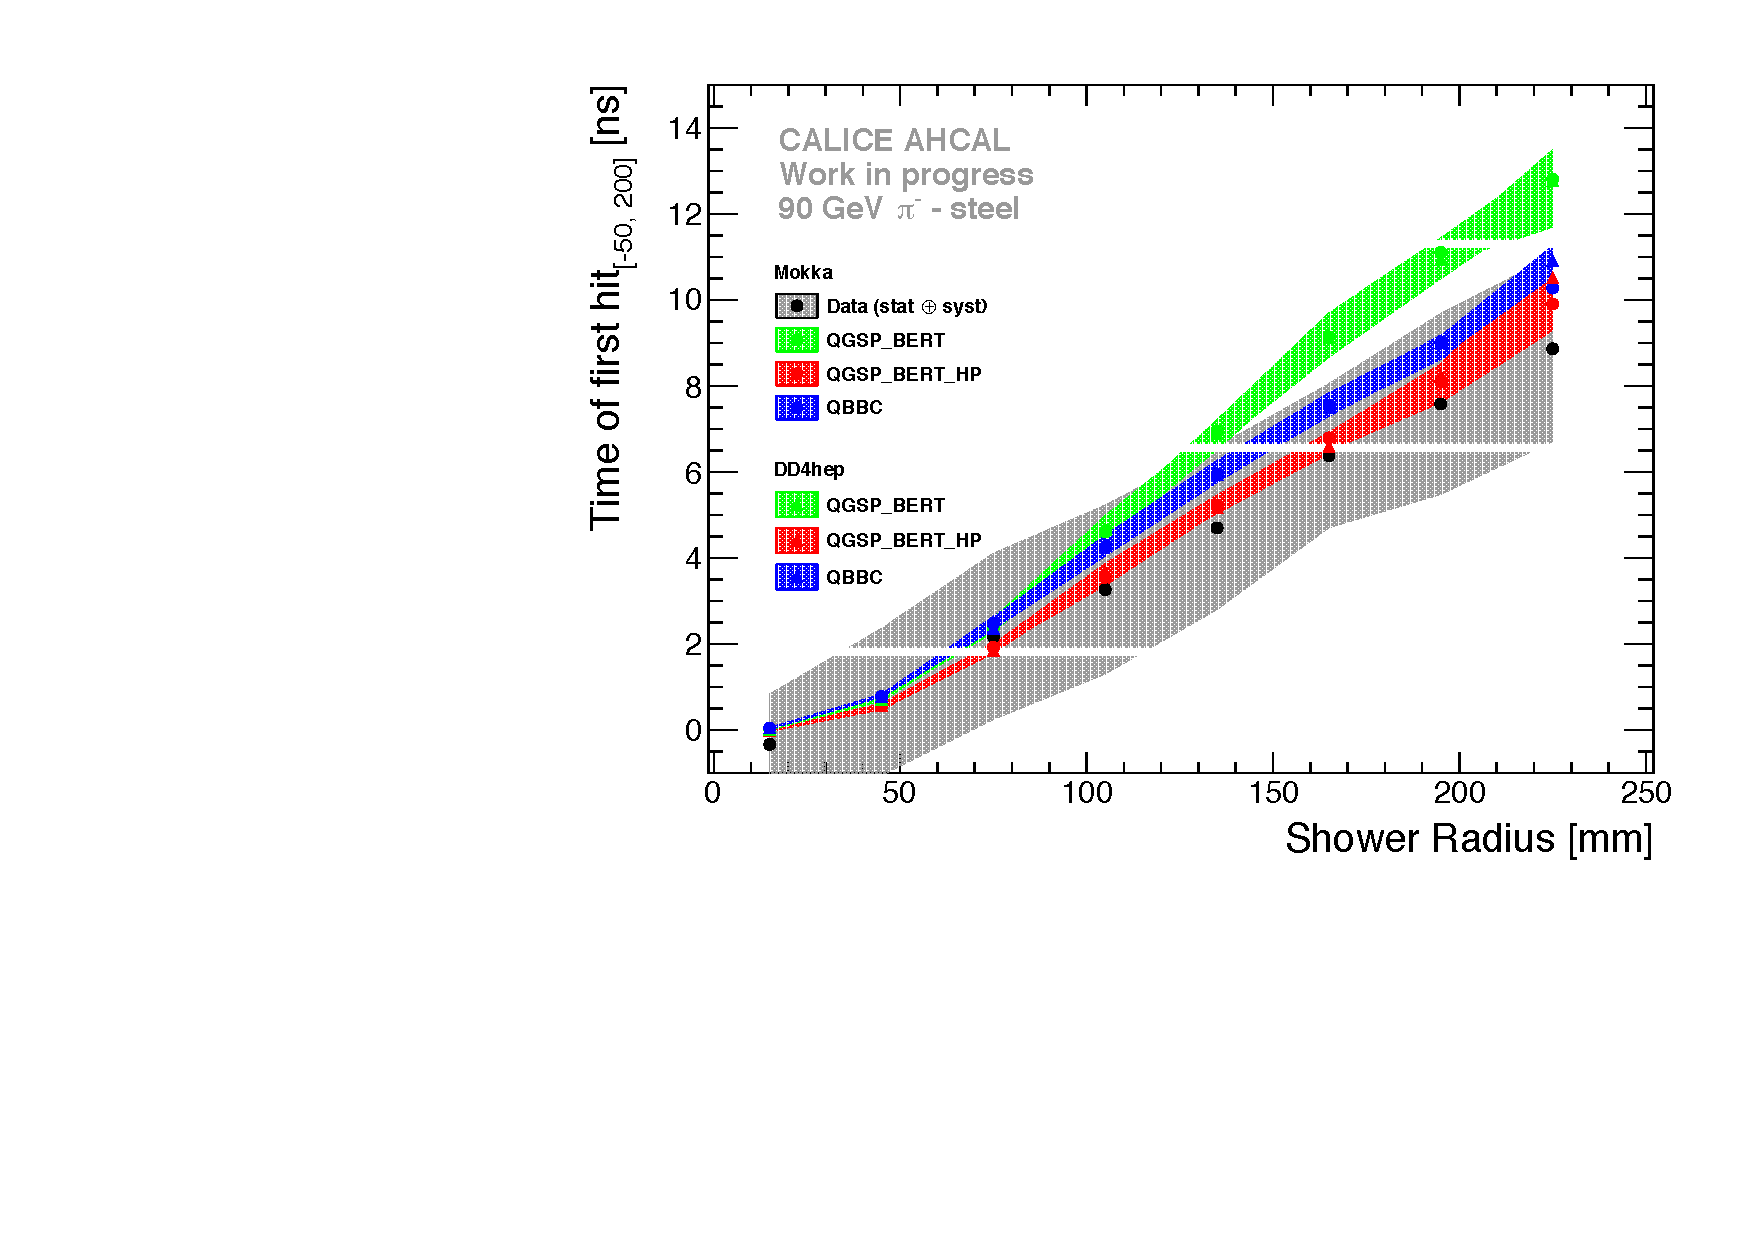
\includegraphics[width=1\textwidth]{chap5/fig_AHCAL_timing/Pions/ComparisonToSim/Time_Radius_90GeV_SSF.pdf}
		\caption{90 GeV (SSF).} \label{fig:Radius_SSF_SimData_90GeV}
	\end{subfigure}
	\caption{Comparison between simulations and data of the time of first hit as function of the distance to the shower axis for pion beams between 10 GeV and 90 GeV for the small layers (layers 3 to 10). The grey and color bands shows the systematics.}
	\label{fig:Radius_SSF_SimData_Comparison}
\end{figure}

\begin{figure}[htbp!]
	\begin{subfigure}[t]{0.5\textwidth}
		\centering
		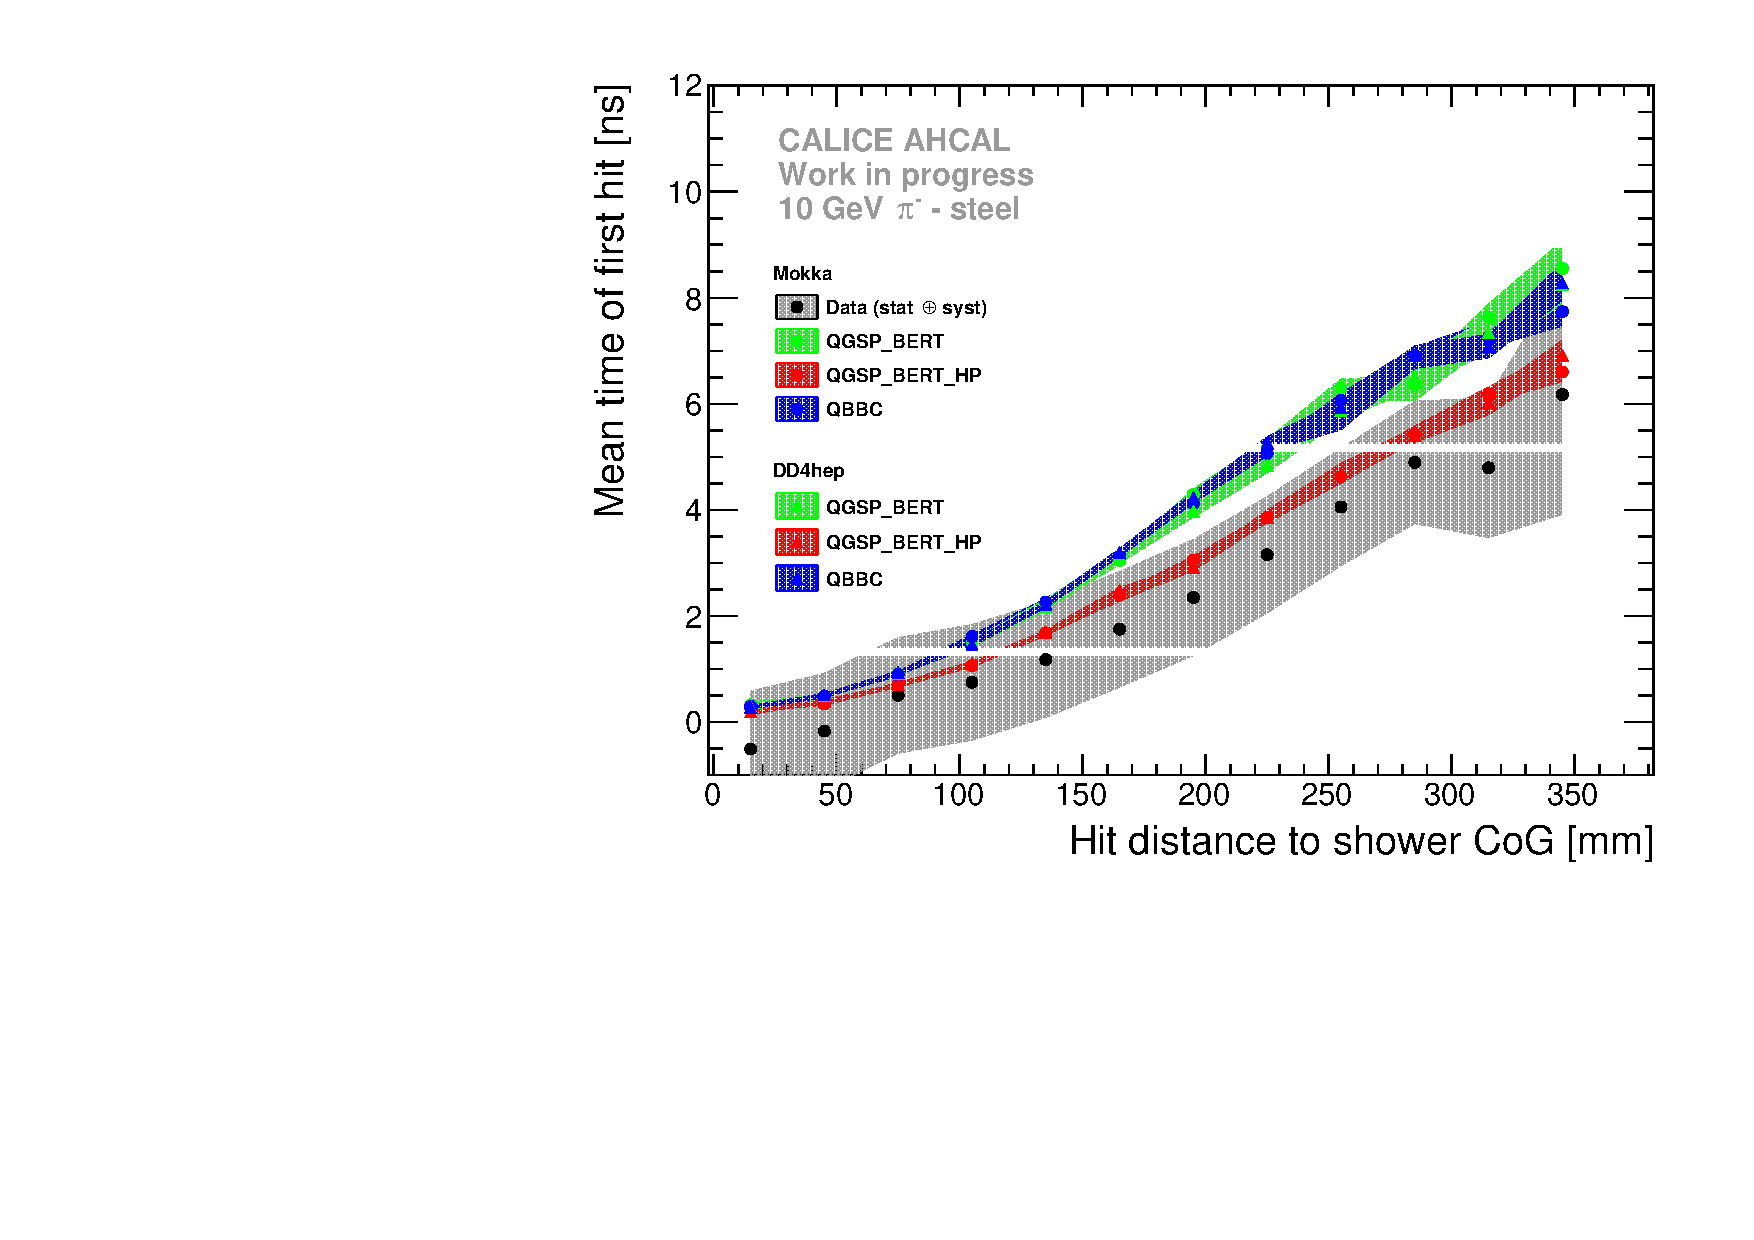
\includegraphics[width=1\textwidth]{chap5/fig_AHCAL_timing/Pions/ComparisonToSim/Time_Radius_10GeV_BL.pdf}
		\caption{10 GeV (BL).}\label{fig:Radius_BL_SimData_10GeV}
	\end{subfigure}
	\hfill
	\begin{subfigure}[t]{0.5\textwidth}
		\centering
		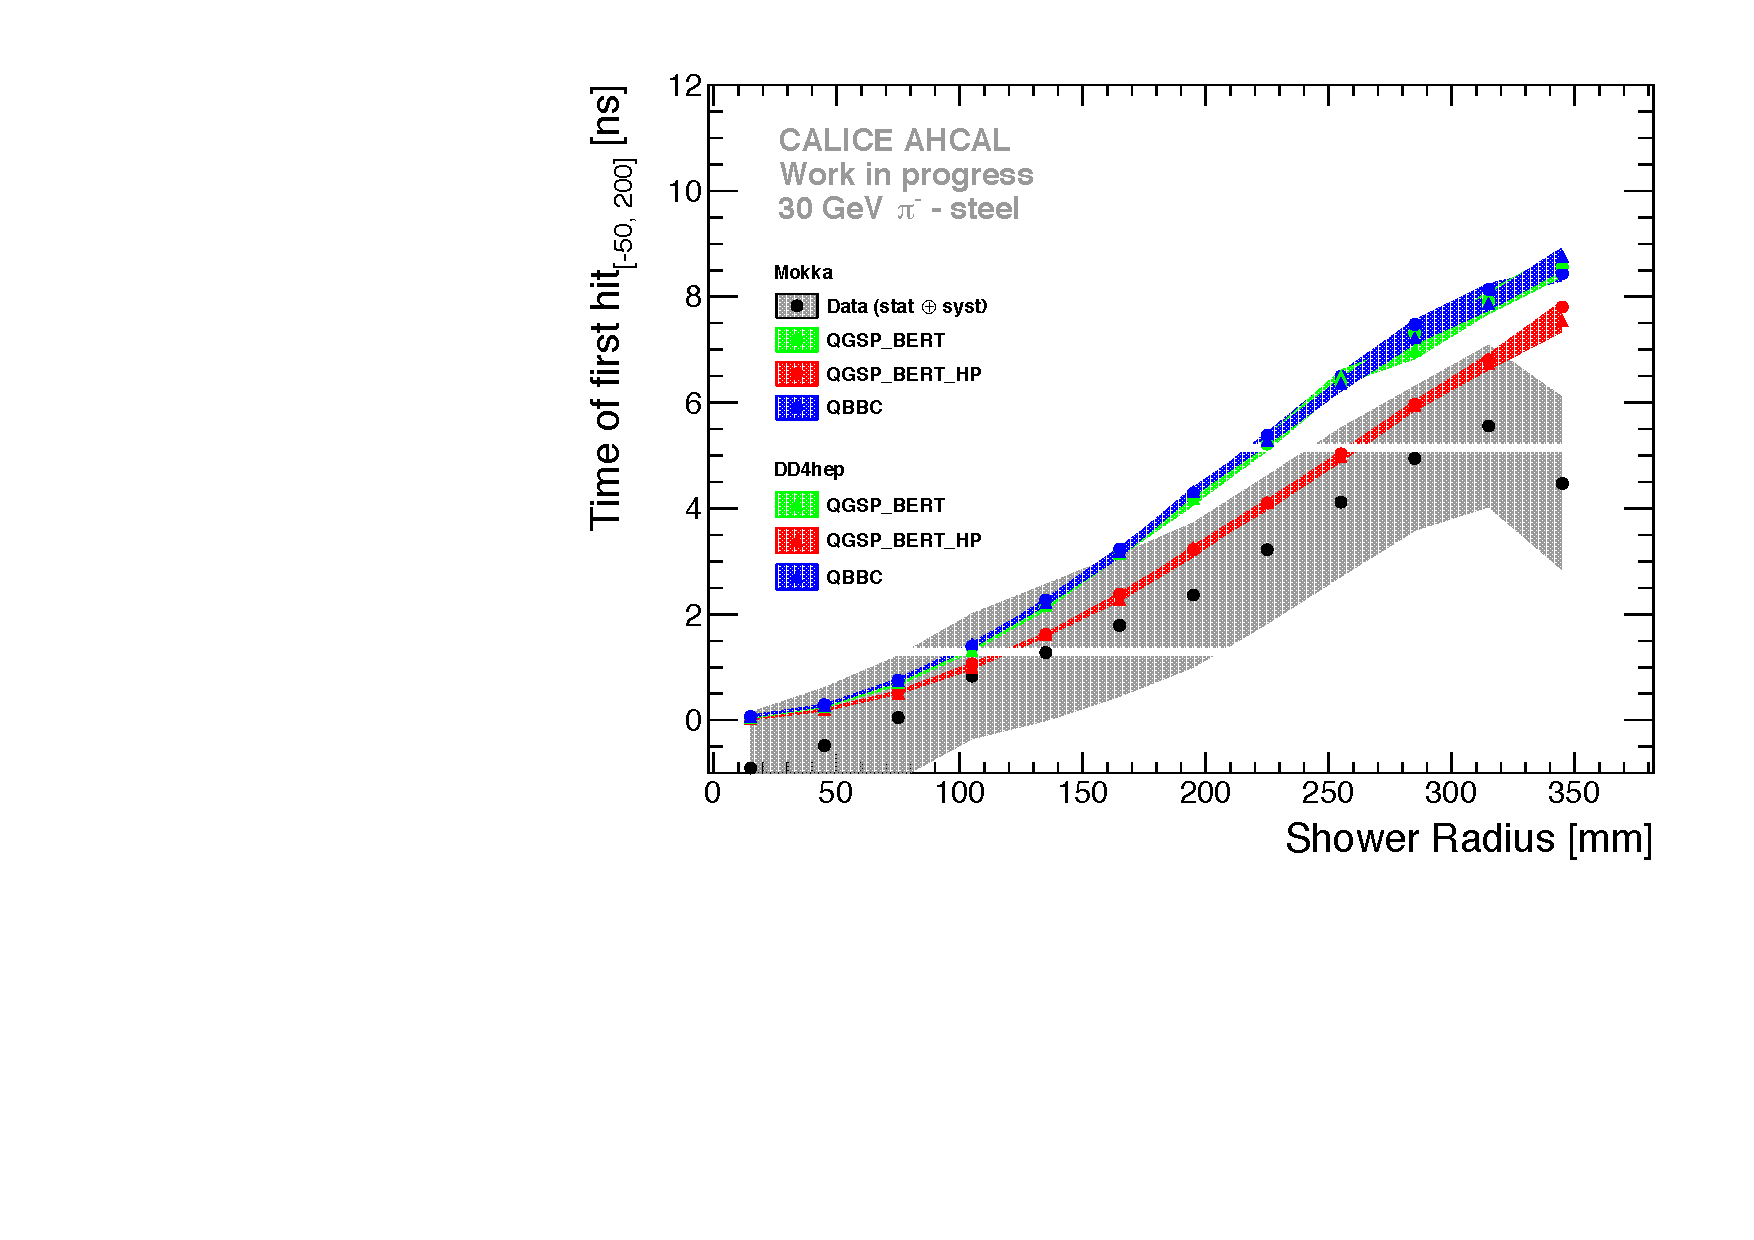
\includegraphics[width=1\textwidth]{chap5/fig_AHCAL_timing/Pions/ComparisonToSim/Time_Radius_30GeV_BL.pdf}
		\caption{30 GeV (BL).} \label{fig:Radius_BL_SimData_30GeV}
	\end{subfigure}
	\hfill
	\begin{subfigure}[t]{0.5\textwidth}
		\centering
		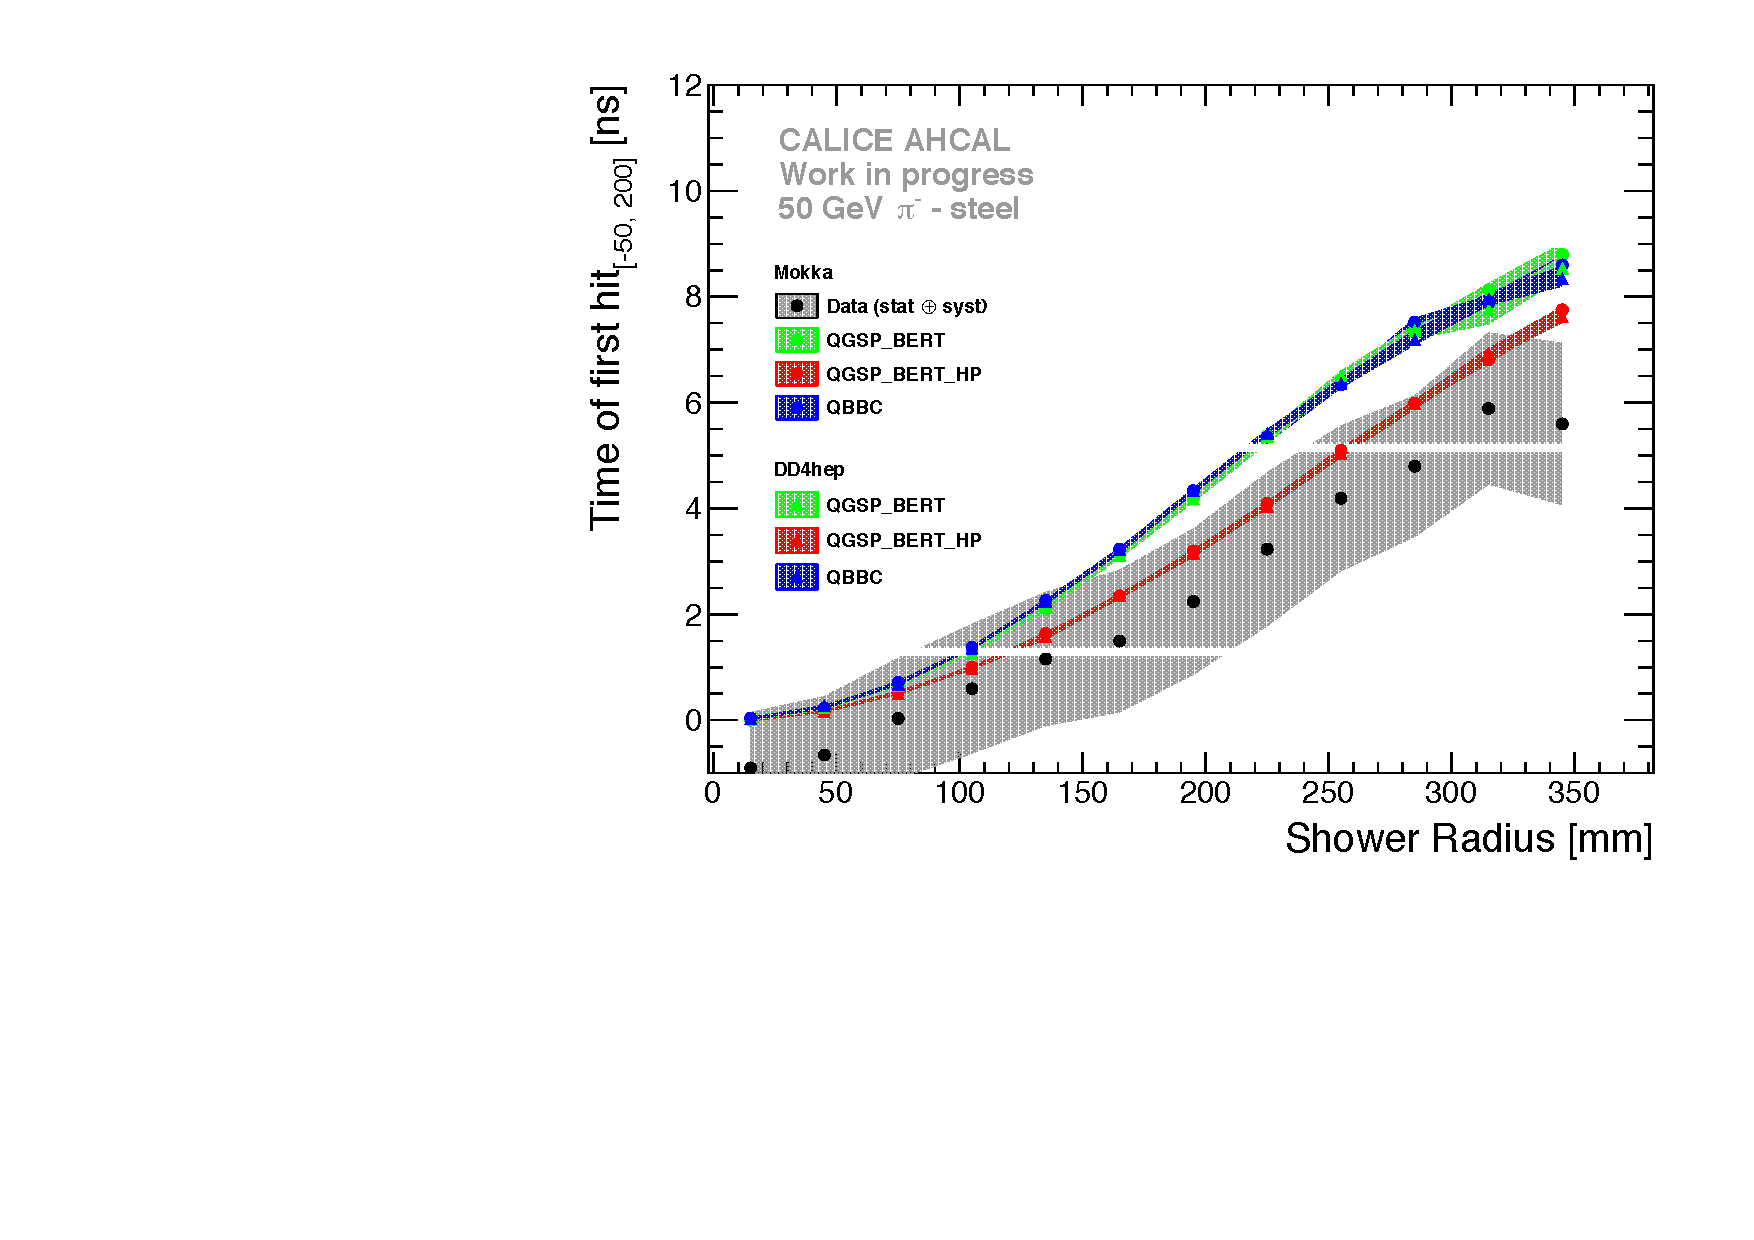
\includegraphics[width=1\textwidth]{chap5/fig_AHCAL_timing/Pions/ComparisonToSim/Time_Radius_50GeV_BL.pdf}
		\caption{50 GeV (BL).} \label{fig:Radius_BL_SimData_50GeV}
	\end{subfigure}
	\hfill
	\begin{subfigure}[t]{0.5\textwidth}
		\centering
		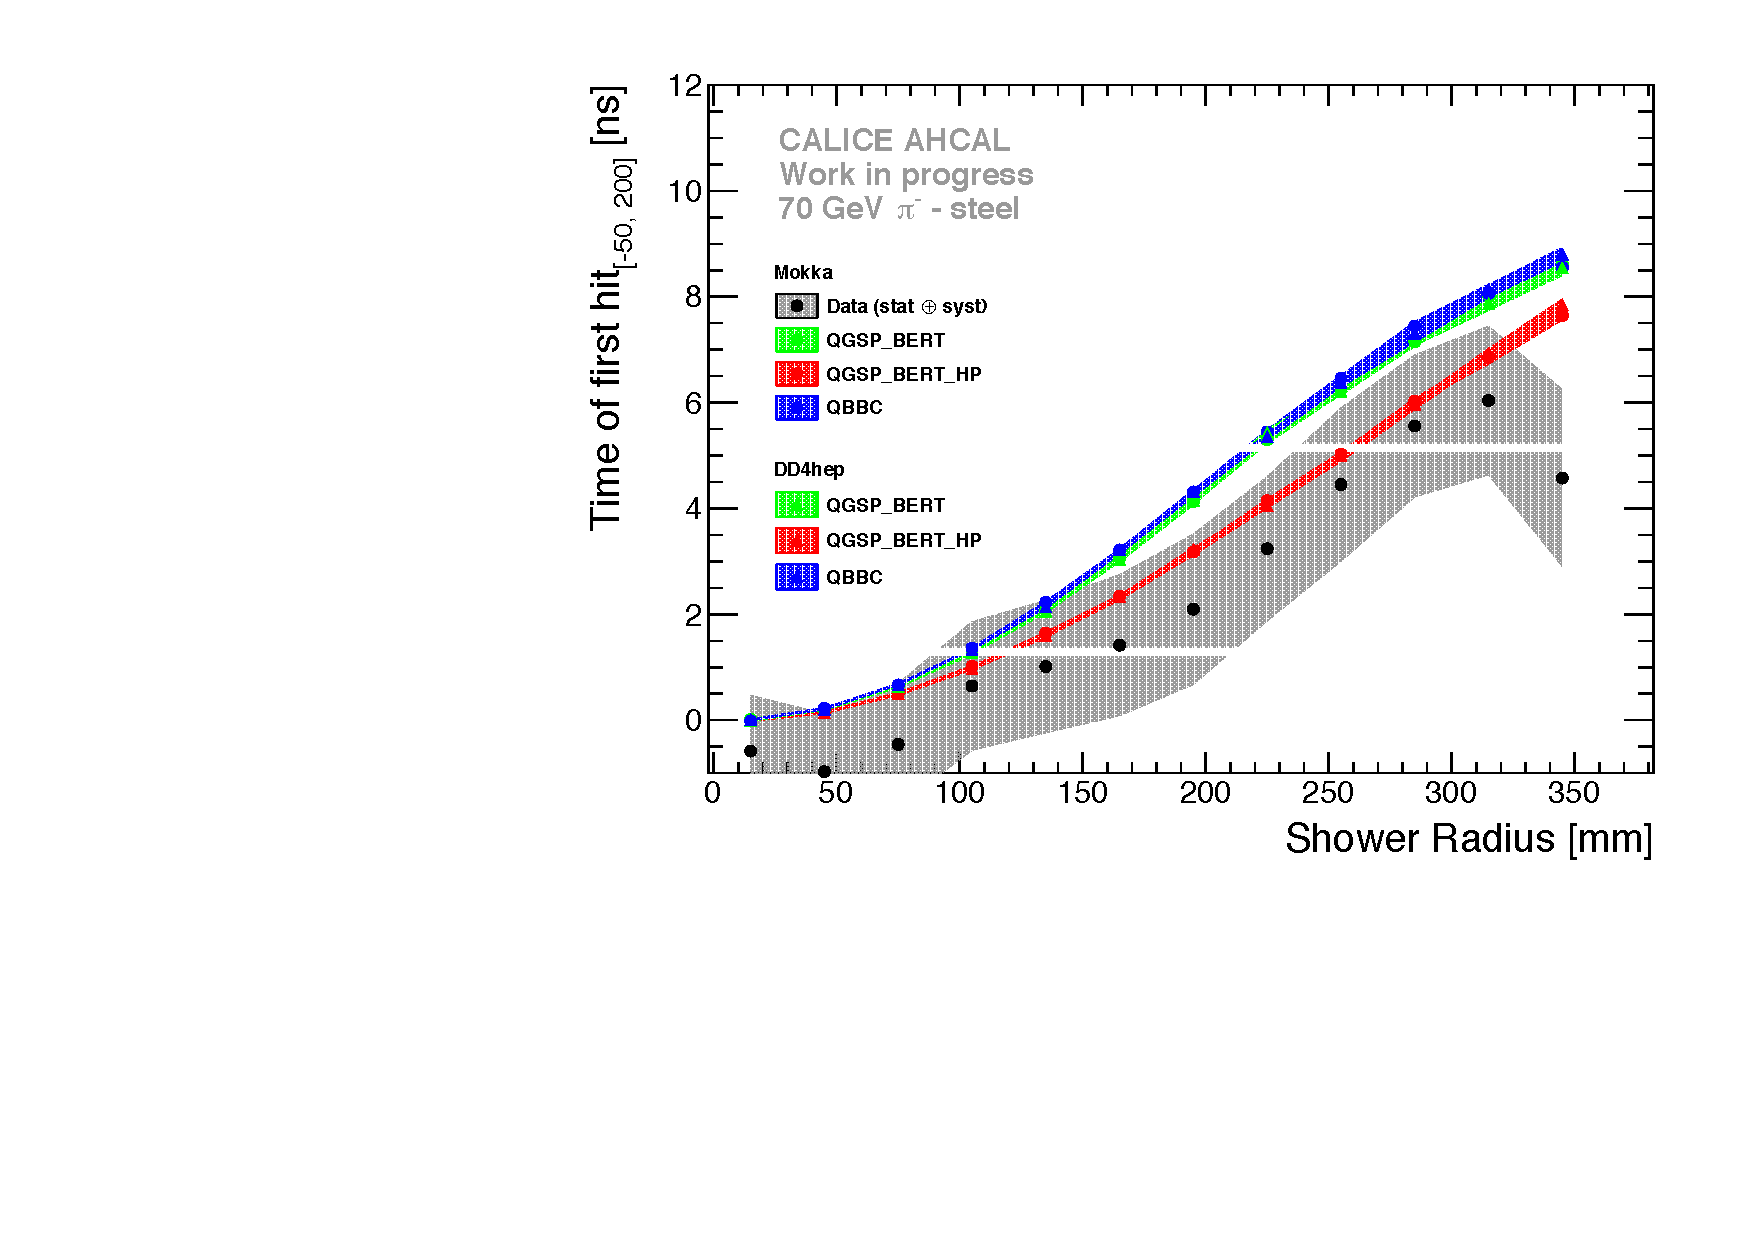
\includegraphics[width=1\textwidth]{chap5/fig_AHCAL_timing/Pions/ComparisonToSim/Time_Radius_70GeV_BL.pdf}
		\caption{70 GeV (BL).} \label{fig:Radius_BL_SimData_70GeV}
	\end{subfigure}
	\hfill
	\begin{subfigure}[t]{0.5\textwidth}
		\centering
		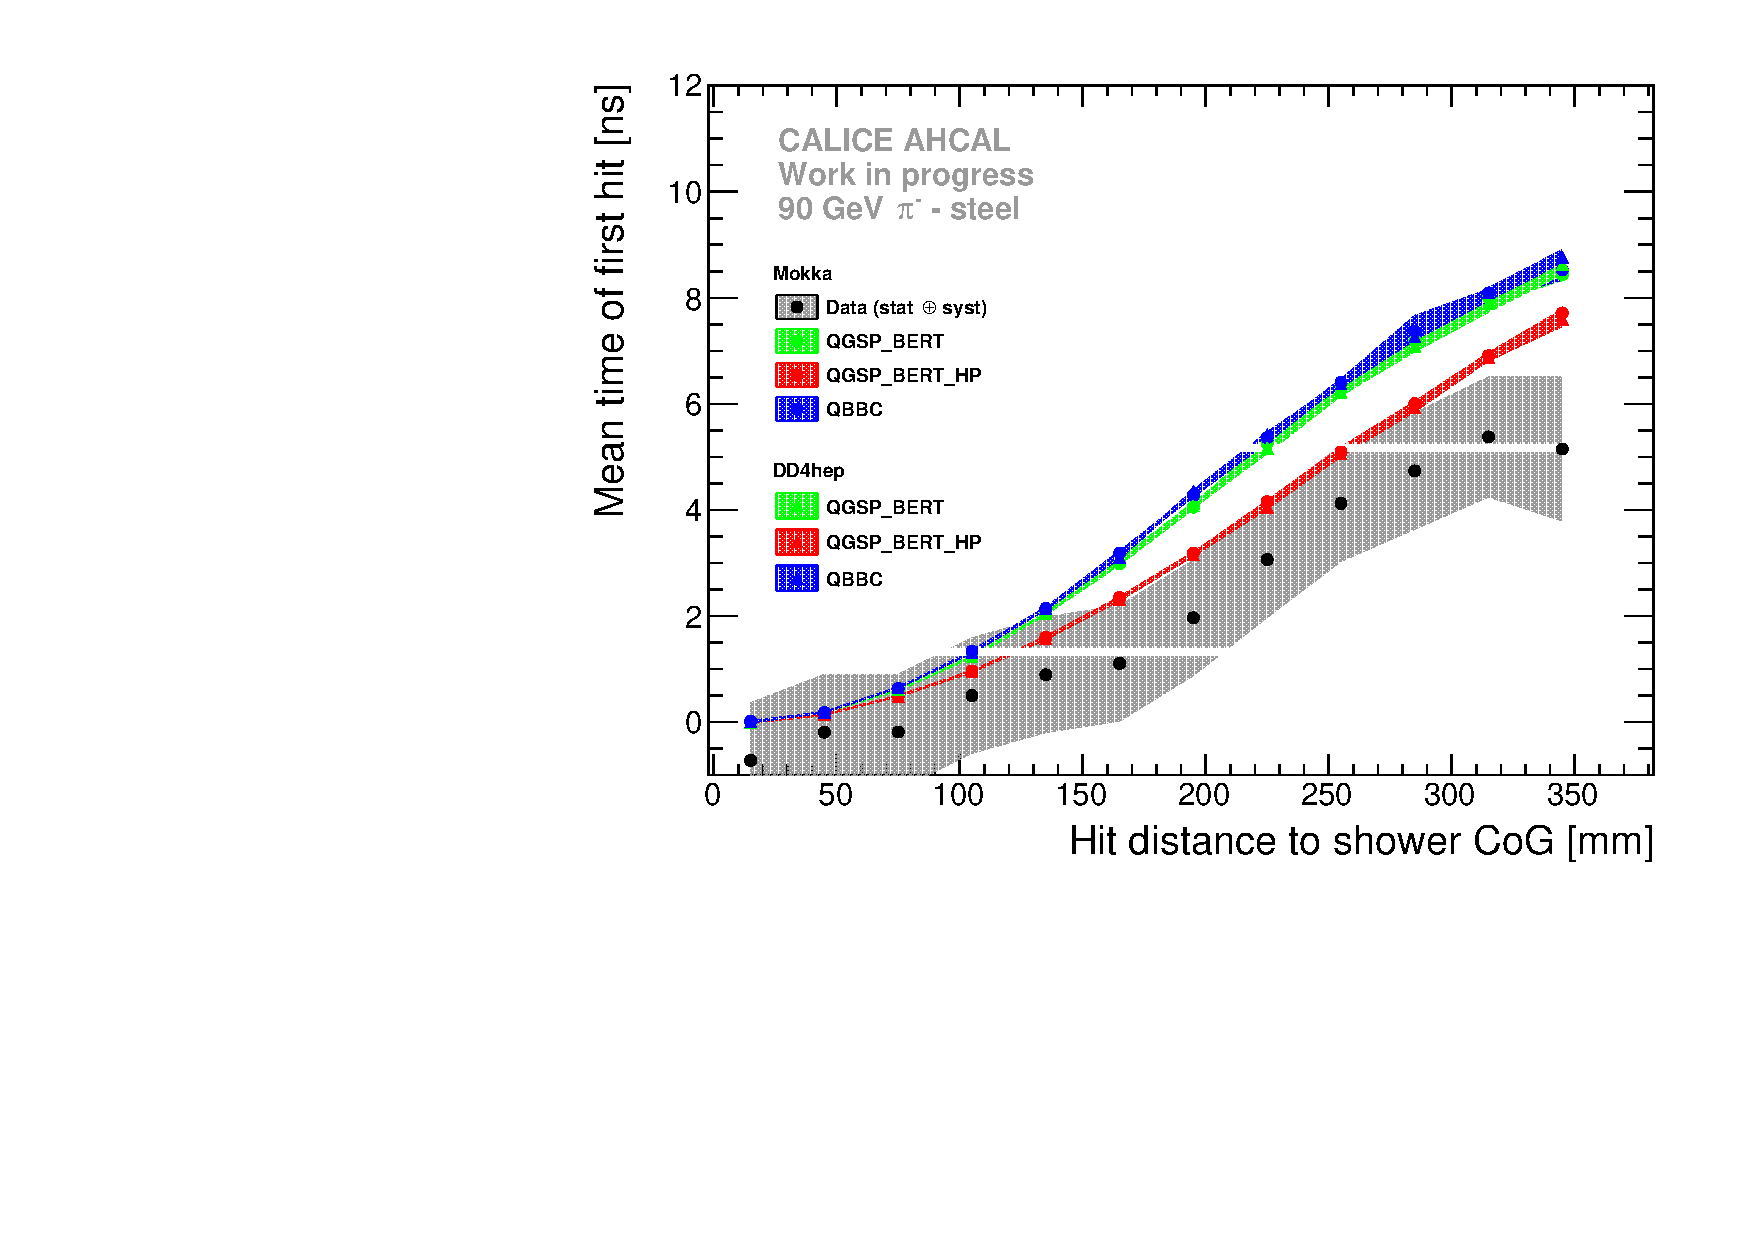
\includegraphics[width=1\textwidth]{chap5/fig_AHCAL_timing/Pions/ComparisonToSim/Time_Radius_90GeV_BL.pdf}
		\caption{90 GeV (BL).} \label{fig:Radius_BL_SimData_90GeV}
	\end{subfigure}
	\caption{Comparison between simulations and data of the time of first hit as function of the distance to the shower axis for pion beams between 10 GeV and 90 GeV for the big layers (layers 11 to 14). The grey and color bands shows the systematics.}
	\label{fig:Radius_BL_SimData_Comparison}
\end{figure}

\begin{figure}[htbp!]
	\begin{subfigure}[t]{0.5\textwidth}
		\centering
		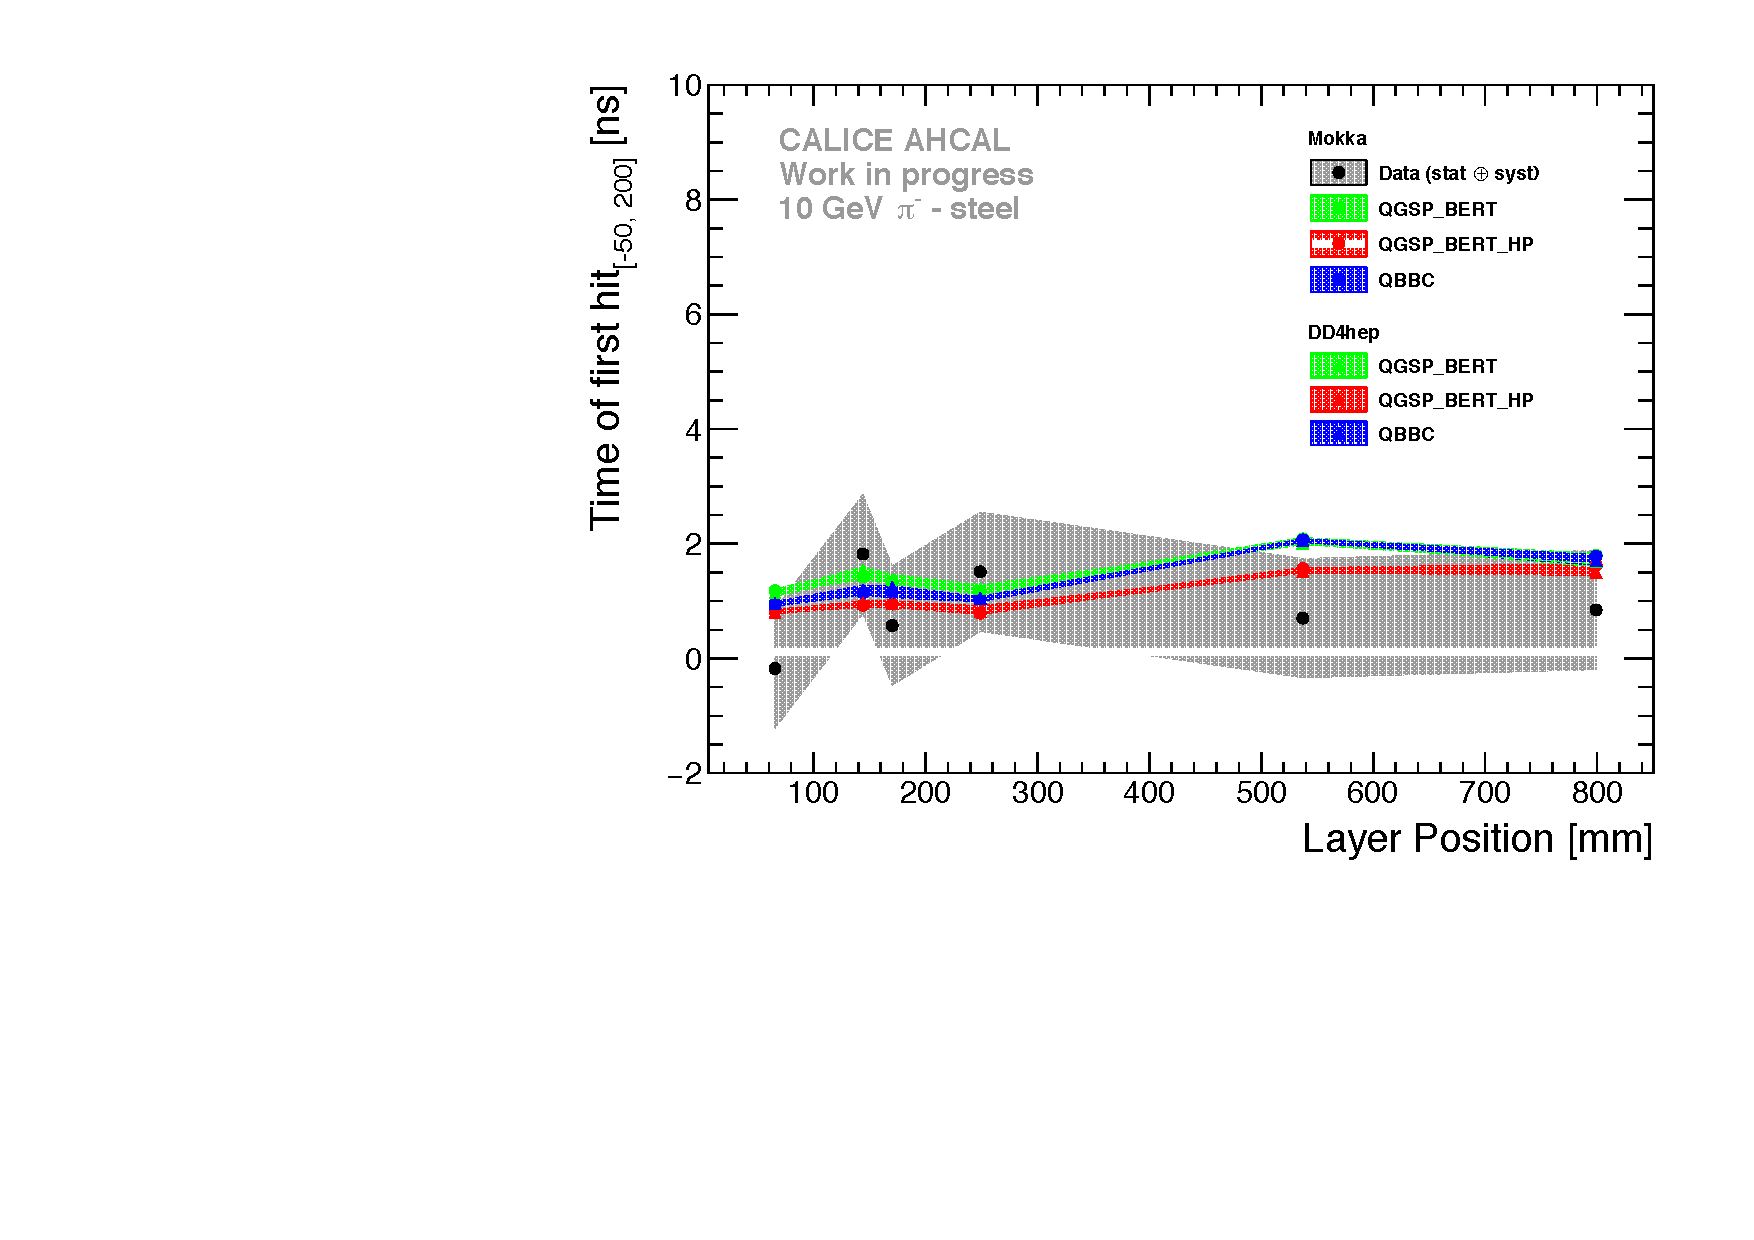
\includegraphics[width=1\textwidth]{chap5/fig_AHCAL_timing/Pions/ComparisonToSim/Time_Depth_10GeV.pdf}
		\caption{10 GeV.}\label{fig:Depth_SimData_10GeV}
	\end{subfigure}
	\hfill
	\begin{subfigure}[t]{0.5\textwidth}
		\centering
		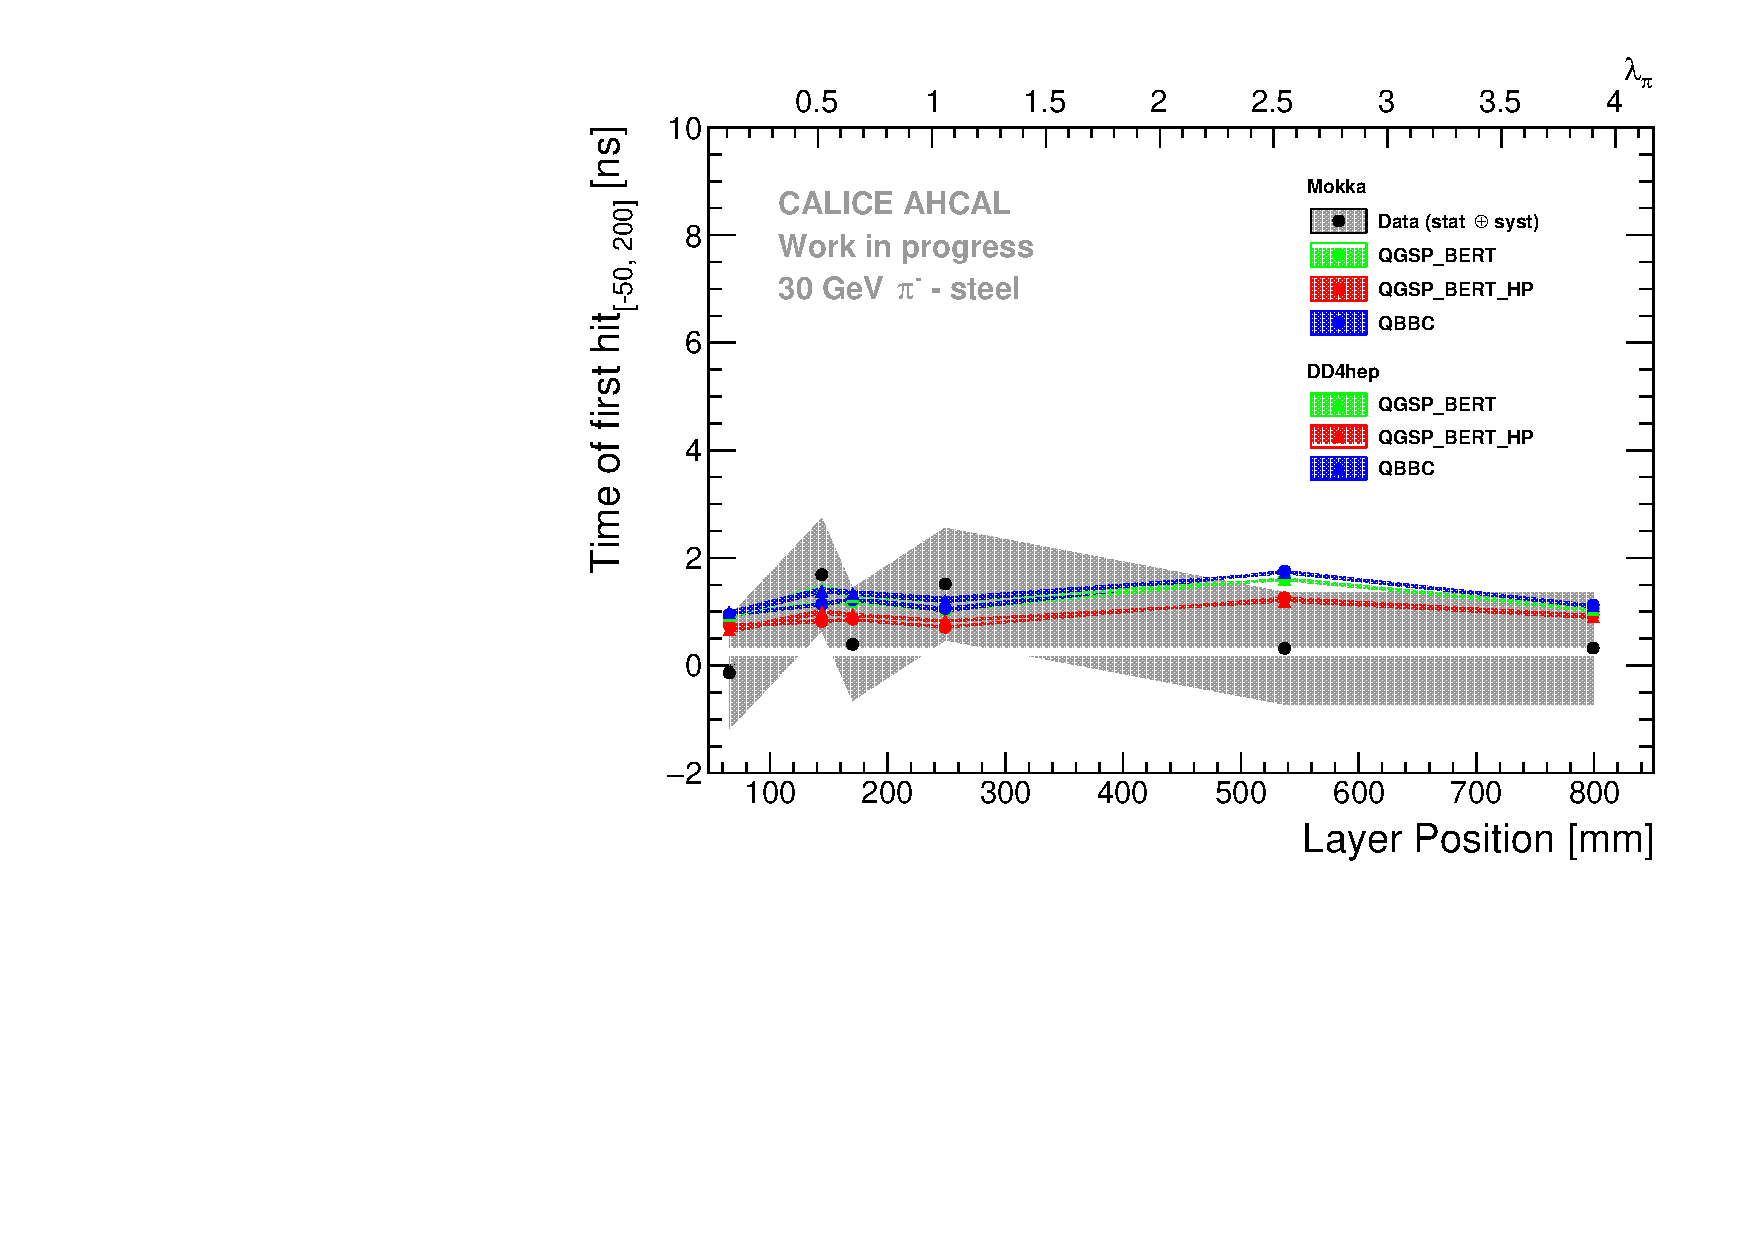
\includegraphics[width=1\textwidth]{chap5/fig_AHCAL_timing/Pions/ComparisonToSim/Time_Depth_30GeV.pdf}
		\caption{30 GeV.} \label{fig:Depth_SimData_30GeV}
	\end{subfigure}
	\hfill
	\begin{subfigure}[t]{0.5\textwidth}
		\centering
		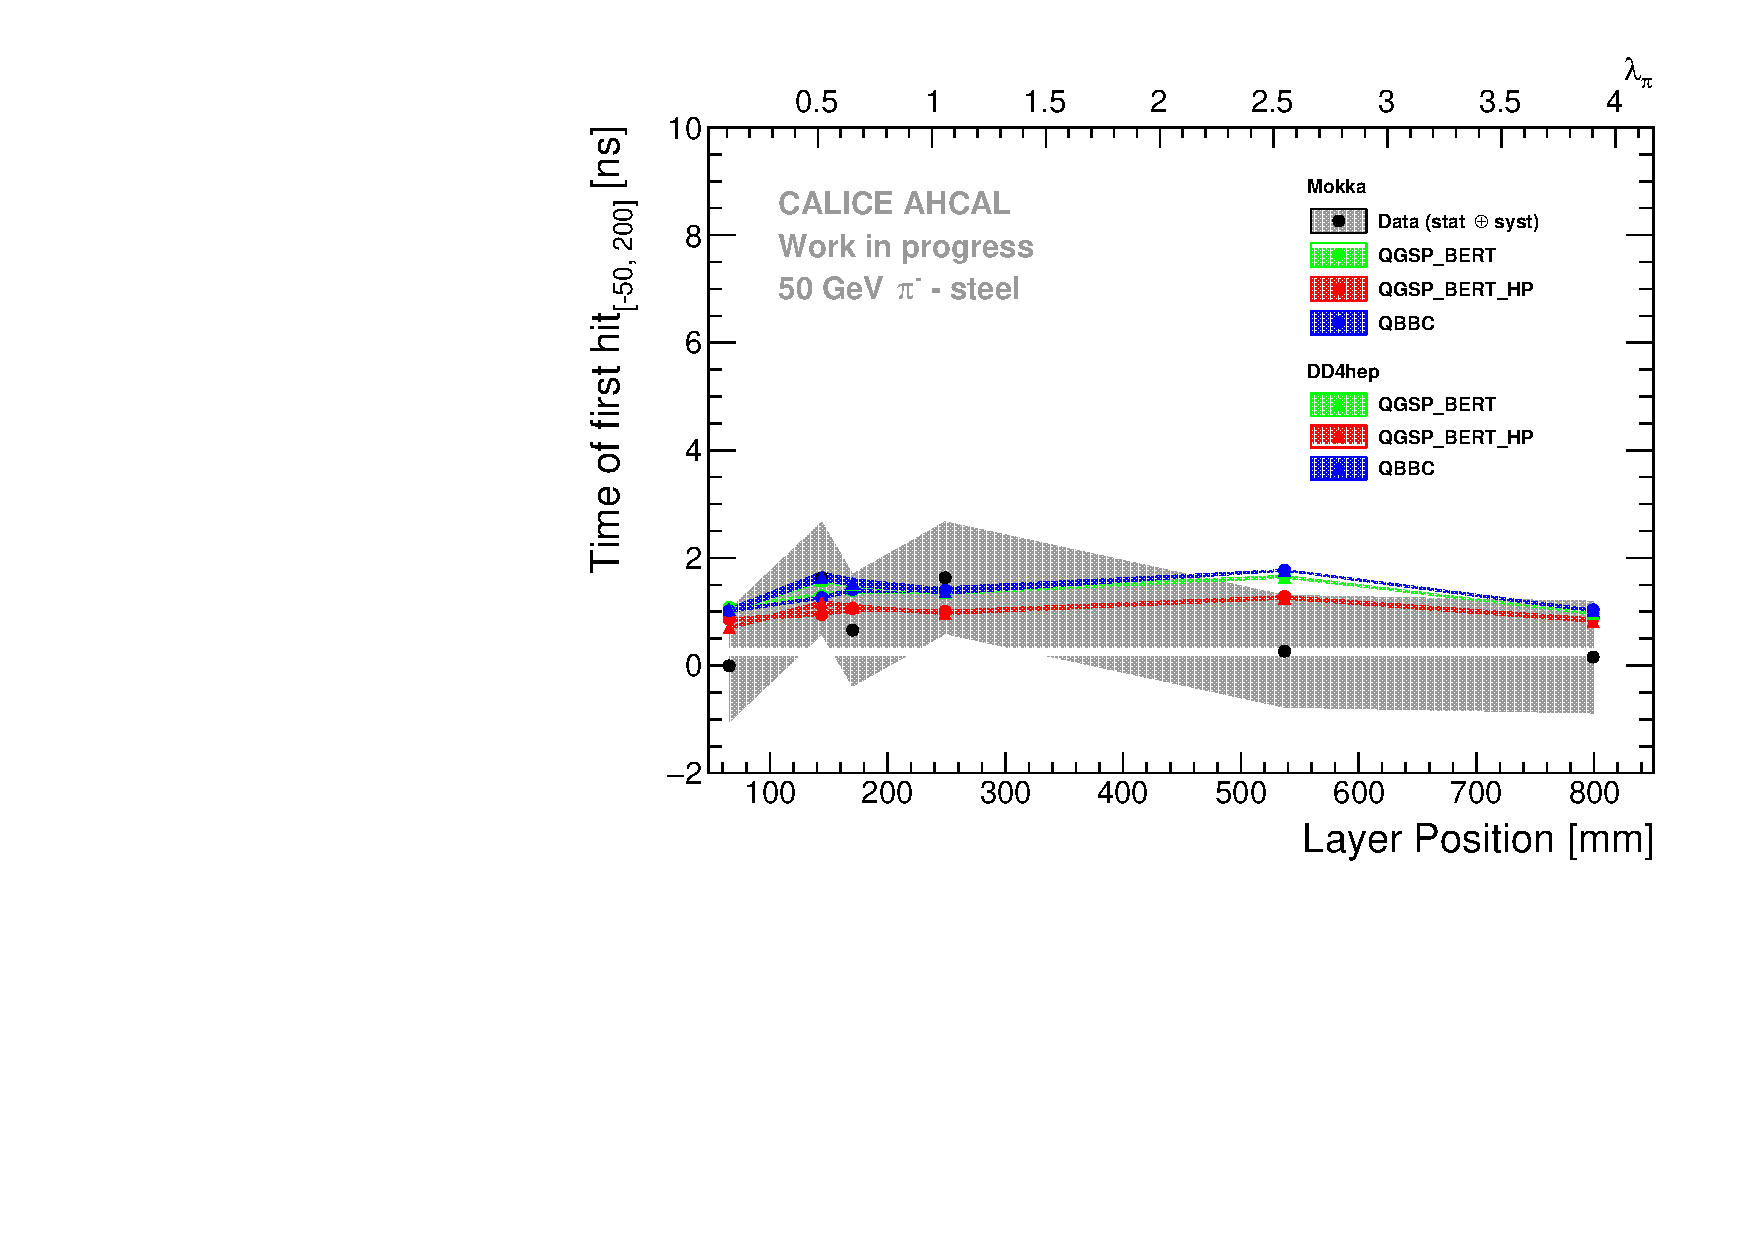
\includegraphics[width=1\textwidth]{chap5/fig_AHCAL_timing/Pions/ComparisonToSim/Time_Depth_50GeV.pdf}
		\caption{50 GeV.} \label{fig:Depth_SimData_50GeV}
	\end{subfigure}
	\hfill
	\begin{subfigure}[t]{0.5\textwidth}
		\centering
		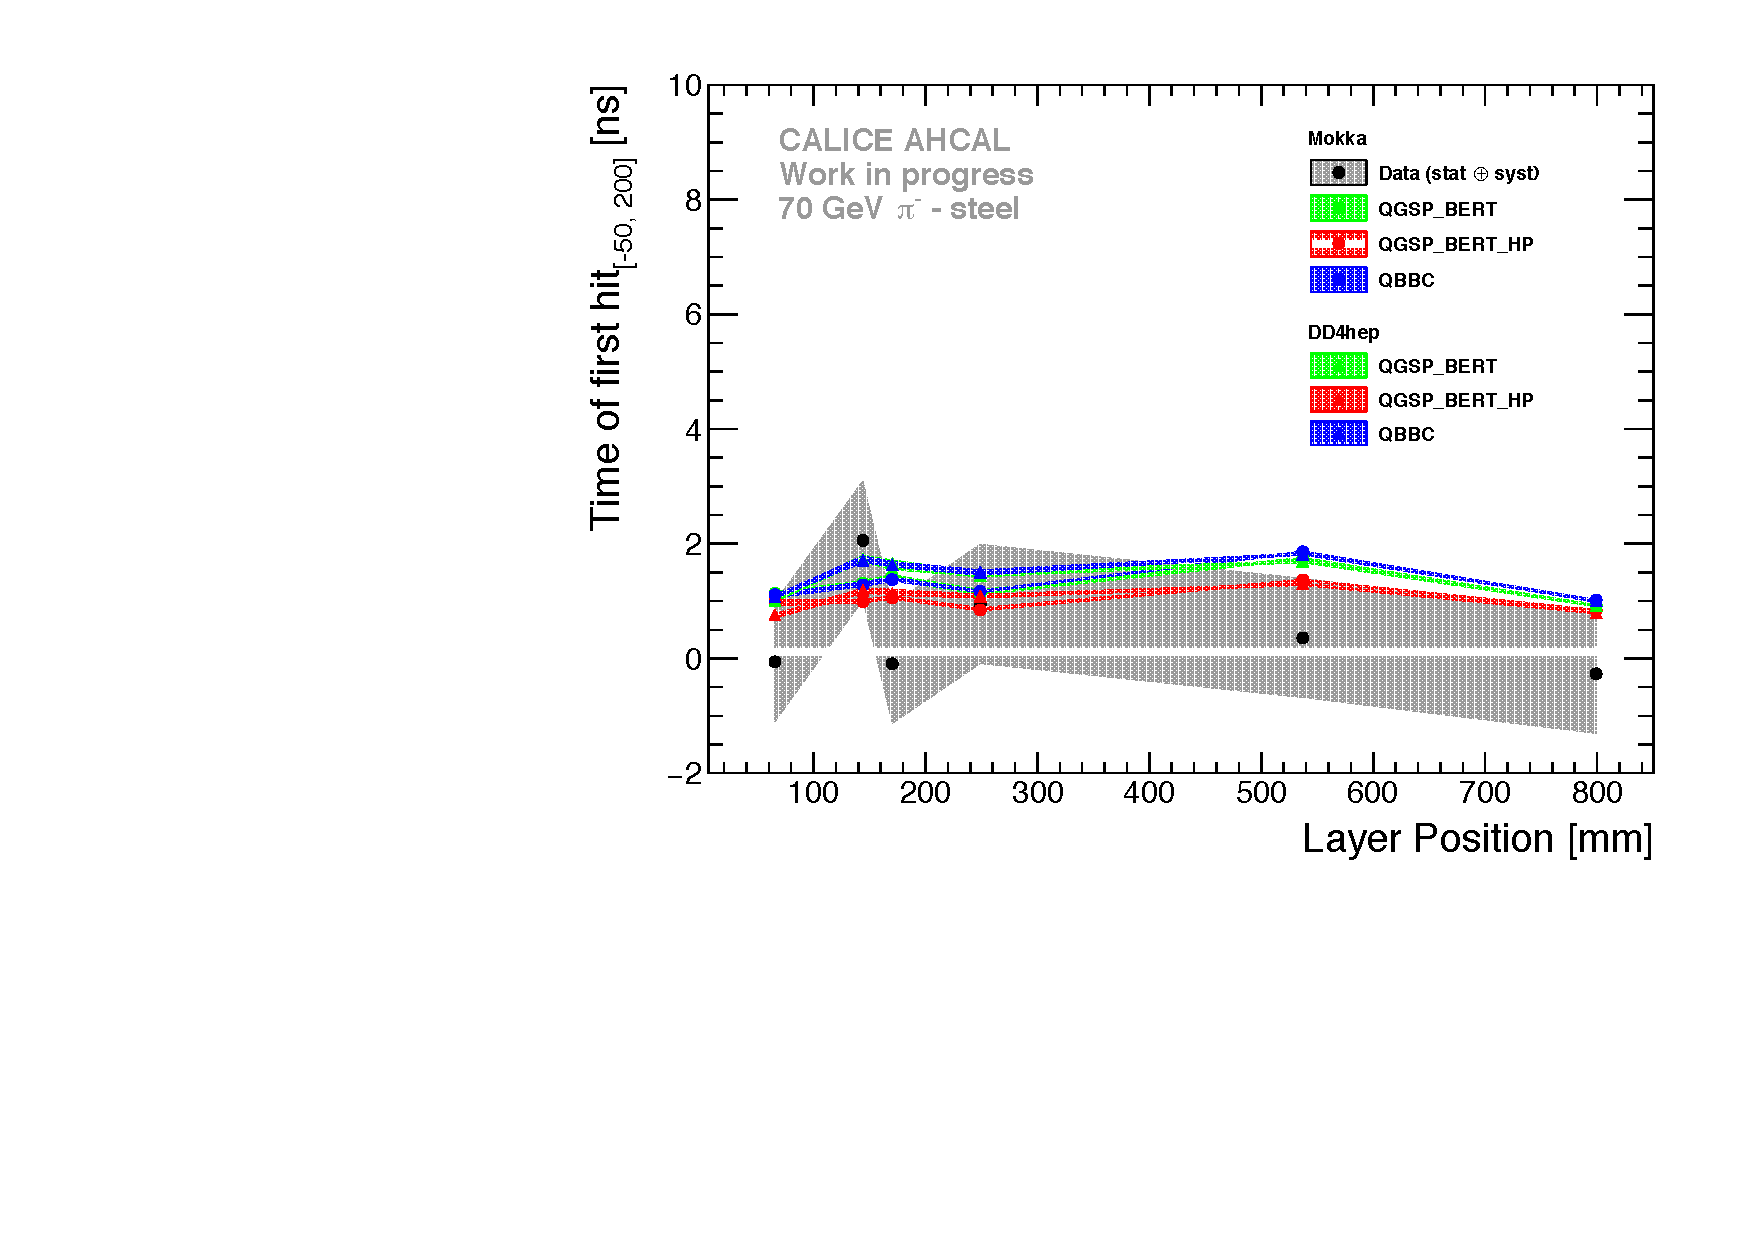
\includegraphics[width=1\textwidth]{chap5/fig_AHCAL_timing/Pions/ComparisonToSim/Time_Depth_70GeV.pdf}
		\caption{70 GeV.} \label{fig:Depth_SimData_70GeV}
	\end{subfigure}
	\hfill
	\begin{subfigure}[t]{0.5\textwidth}
		\centering
		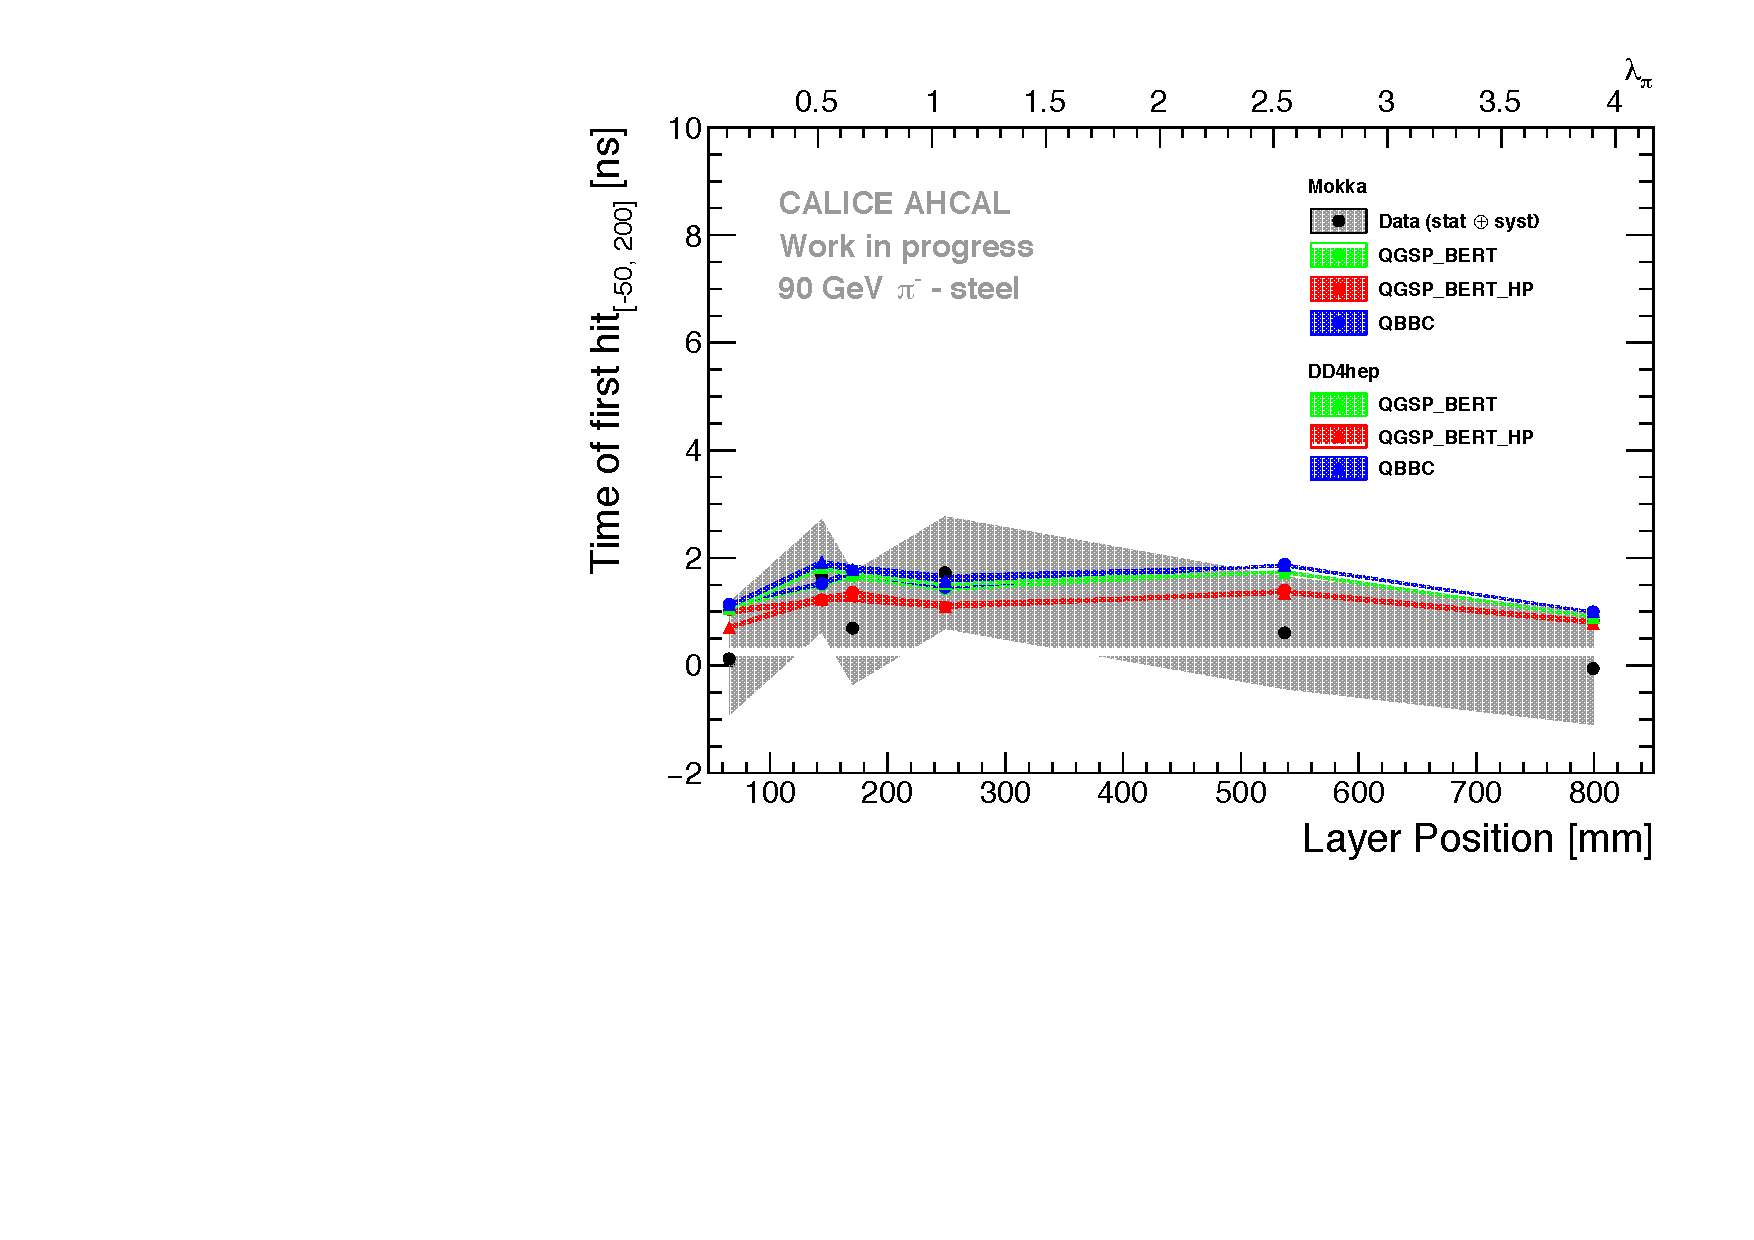
\includegraphics[width=1\textwidth]{chap5/fig_AHCAL_timing/Pions/ComparisonToSim/Time_Depth_90GeV.pdf}
		\caption{90 GeV.} \label{fig:Depth_SimData_90GeV}
	\end{subfigure}
	\caption{Comparison between simulations and data of the time of first hit as function of the layer position for pion beams between 10 GeV and 90 GeV. The grey and color bands shows the systematics.}
	\label{fig:Depth_SimData_Comparison}
\end{figure}

\begin{figure}[htbp!]
	\begin{subfigure}[t]{0.5\textwidth}
		\centering
		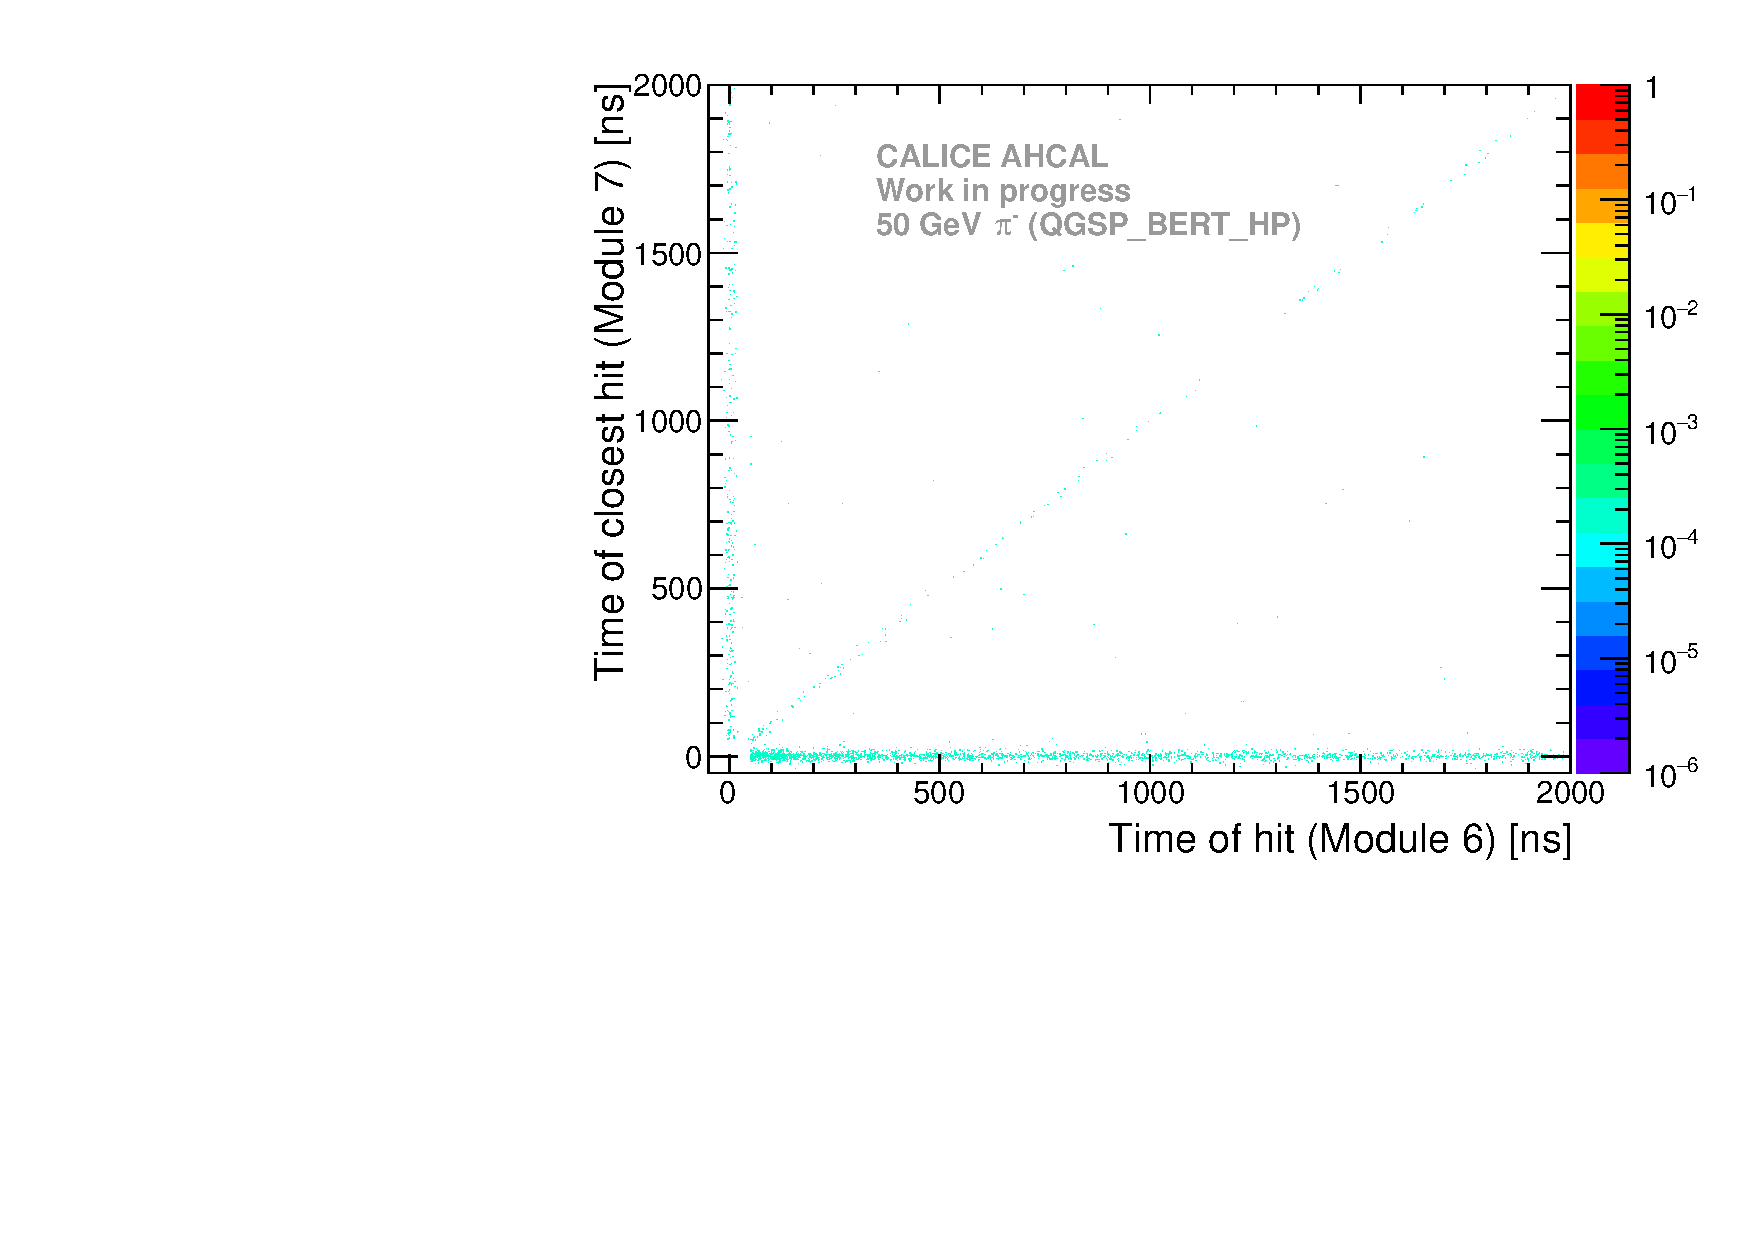
\includegraphics[width=1\textwidth]{chap5/fig_AHCAL_timing/Pions/ComparisonToSim/Time_Correlation_50GeV_short_QGSPBERTHP.pdf}
		\caption{Short correlation (QGSP\_BERT\_HP).} \label{fig:Corr_short_QGSPBERTHP}
	\end{subfigure}
	\hfill
	\begin{subfigure}[t]{0.5\textwidth}
		\centering
		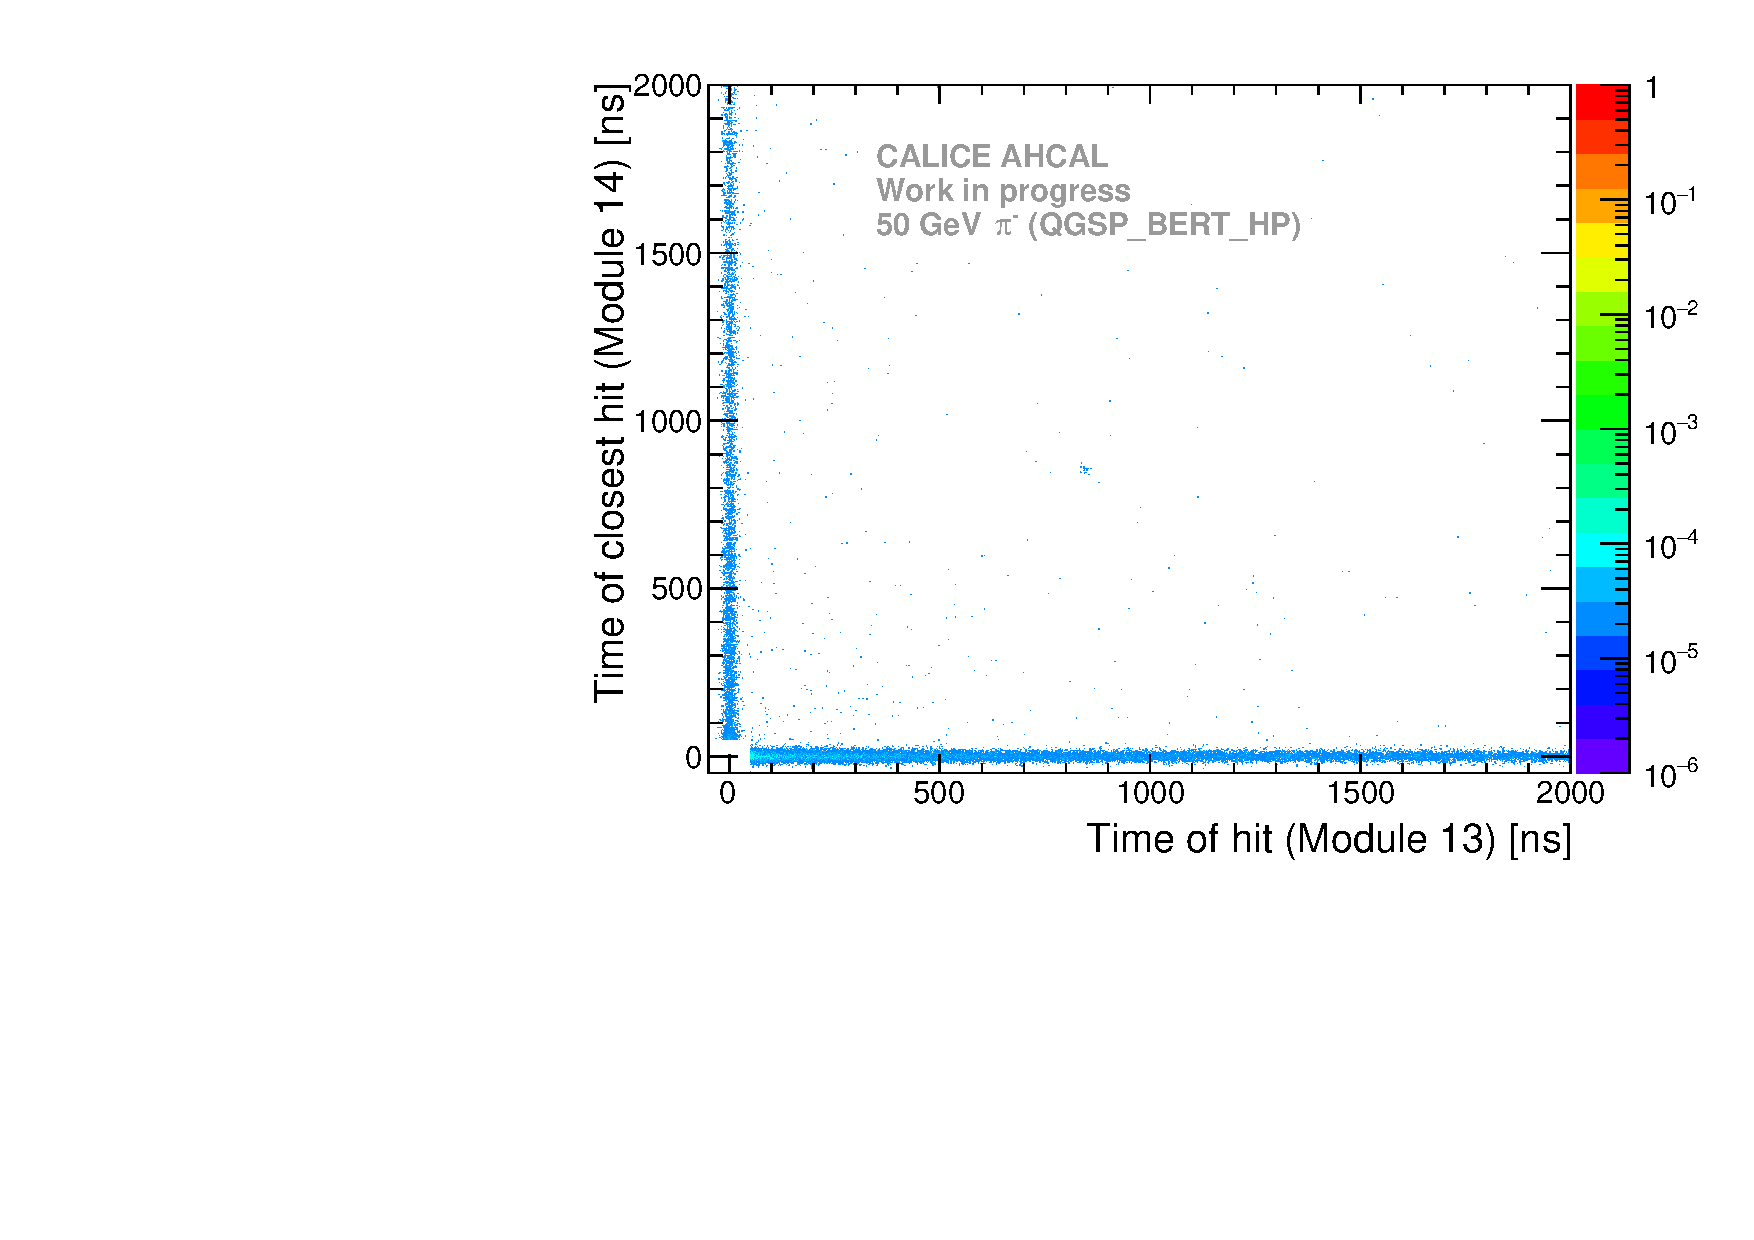
\includegraphics[width=1\textwidth]{chap5/fig_AHCAL_timing/Pions/ComparisonToSim/Time_Correlation_50GeV_long_QGSPBERTHP.pdf}
		\caption{Long correlation (QGSP\_BERT\_HP).} \label{fig:Corr_long_QGSPBERTHP}
	\end{subfigure}
	\hfill
	\begin{subfigure}[t]{0.5\textwidth}
		\centering
		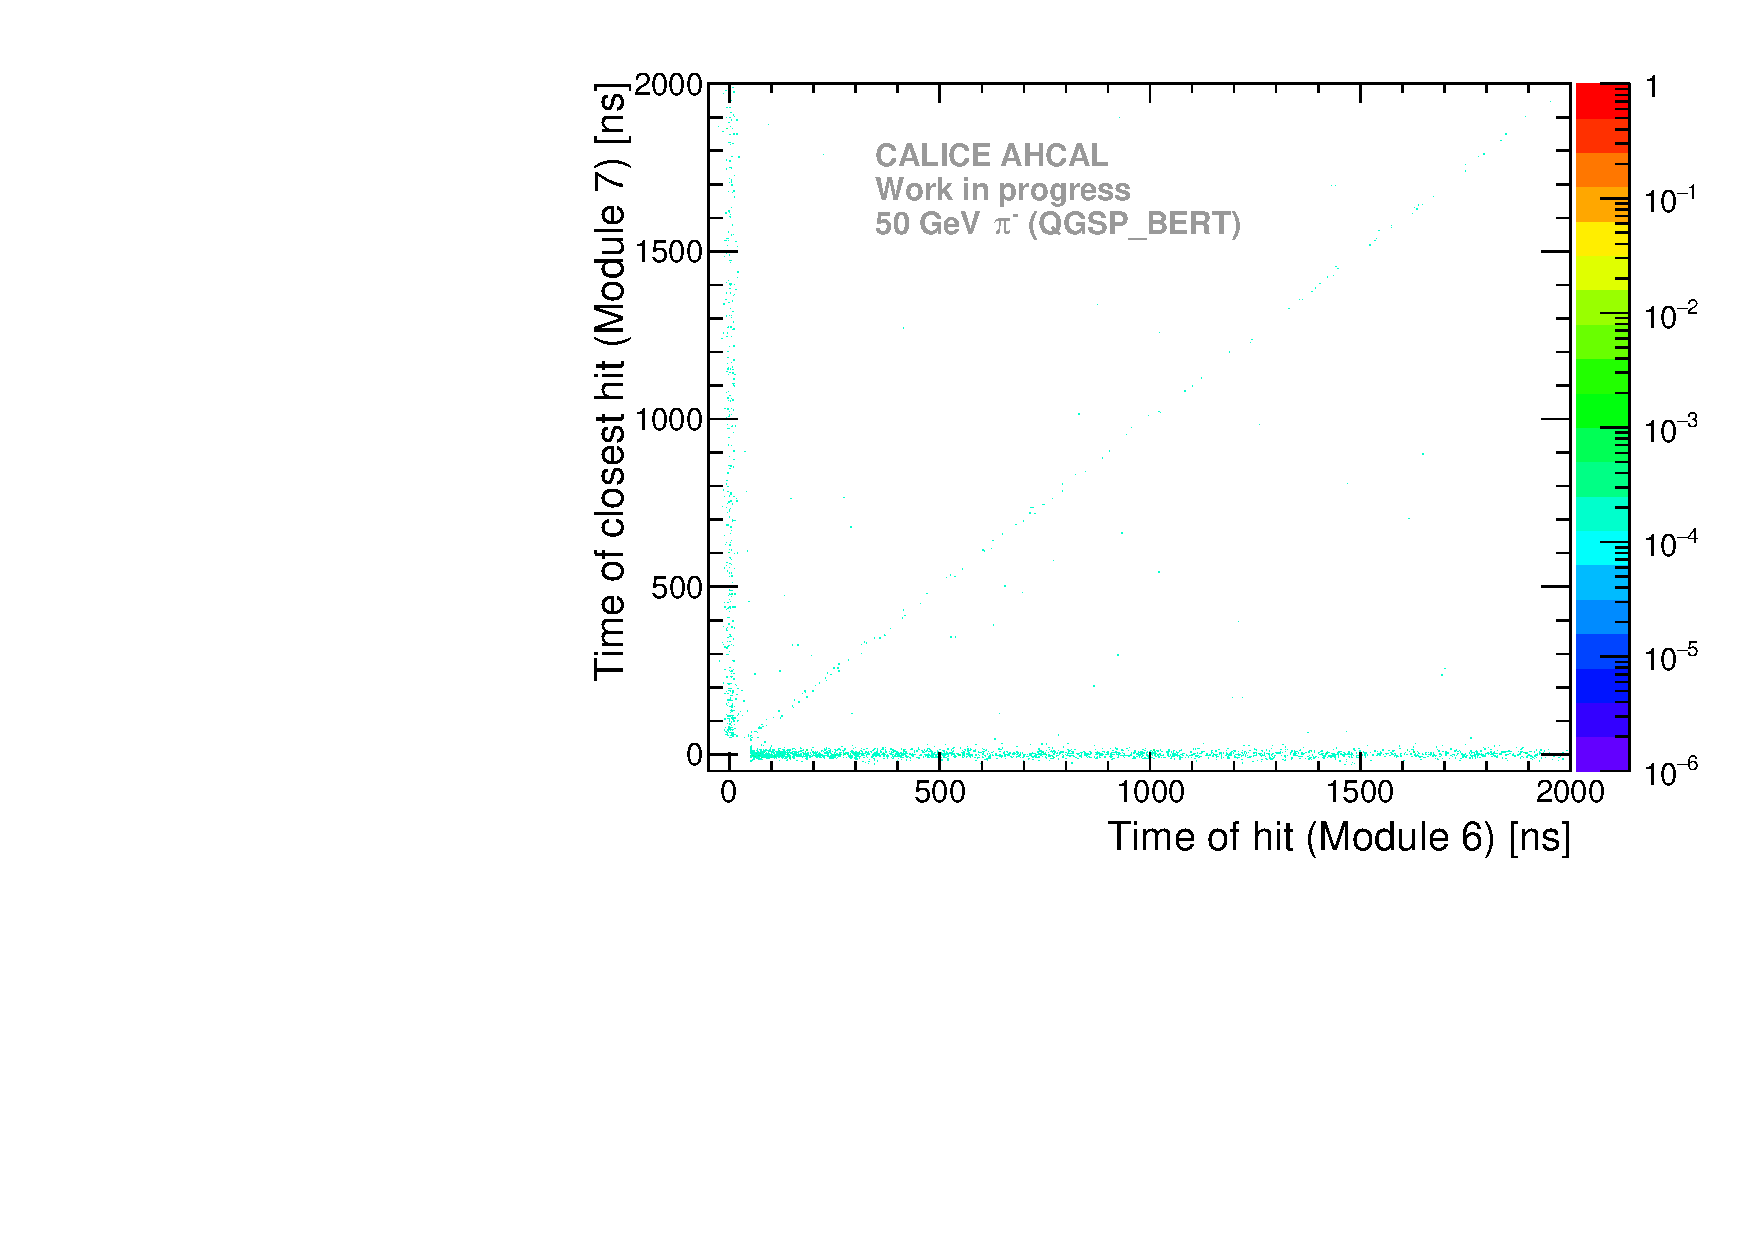
\includegraphics[width=1\textwidth]{chap5/fig_AHCAL_timing/Pions/ComparisonToSim/Time_Correlation_50GeV_short_QGSPBERT.pdf}
		\caption{Short correlation (QGSP\_BERT).}\label{fig:Corr_short_QGSPBERT}
	\end{subfigure}
	\hfill
	\begin{subfigure}[t]{0.5\textwidth}
		\centering
		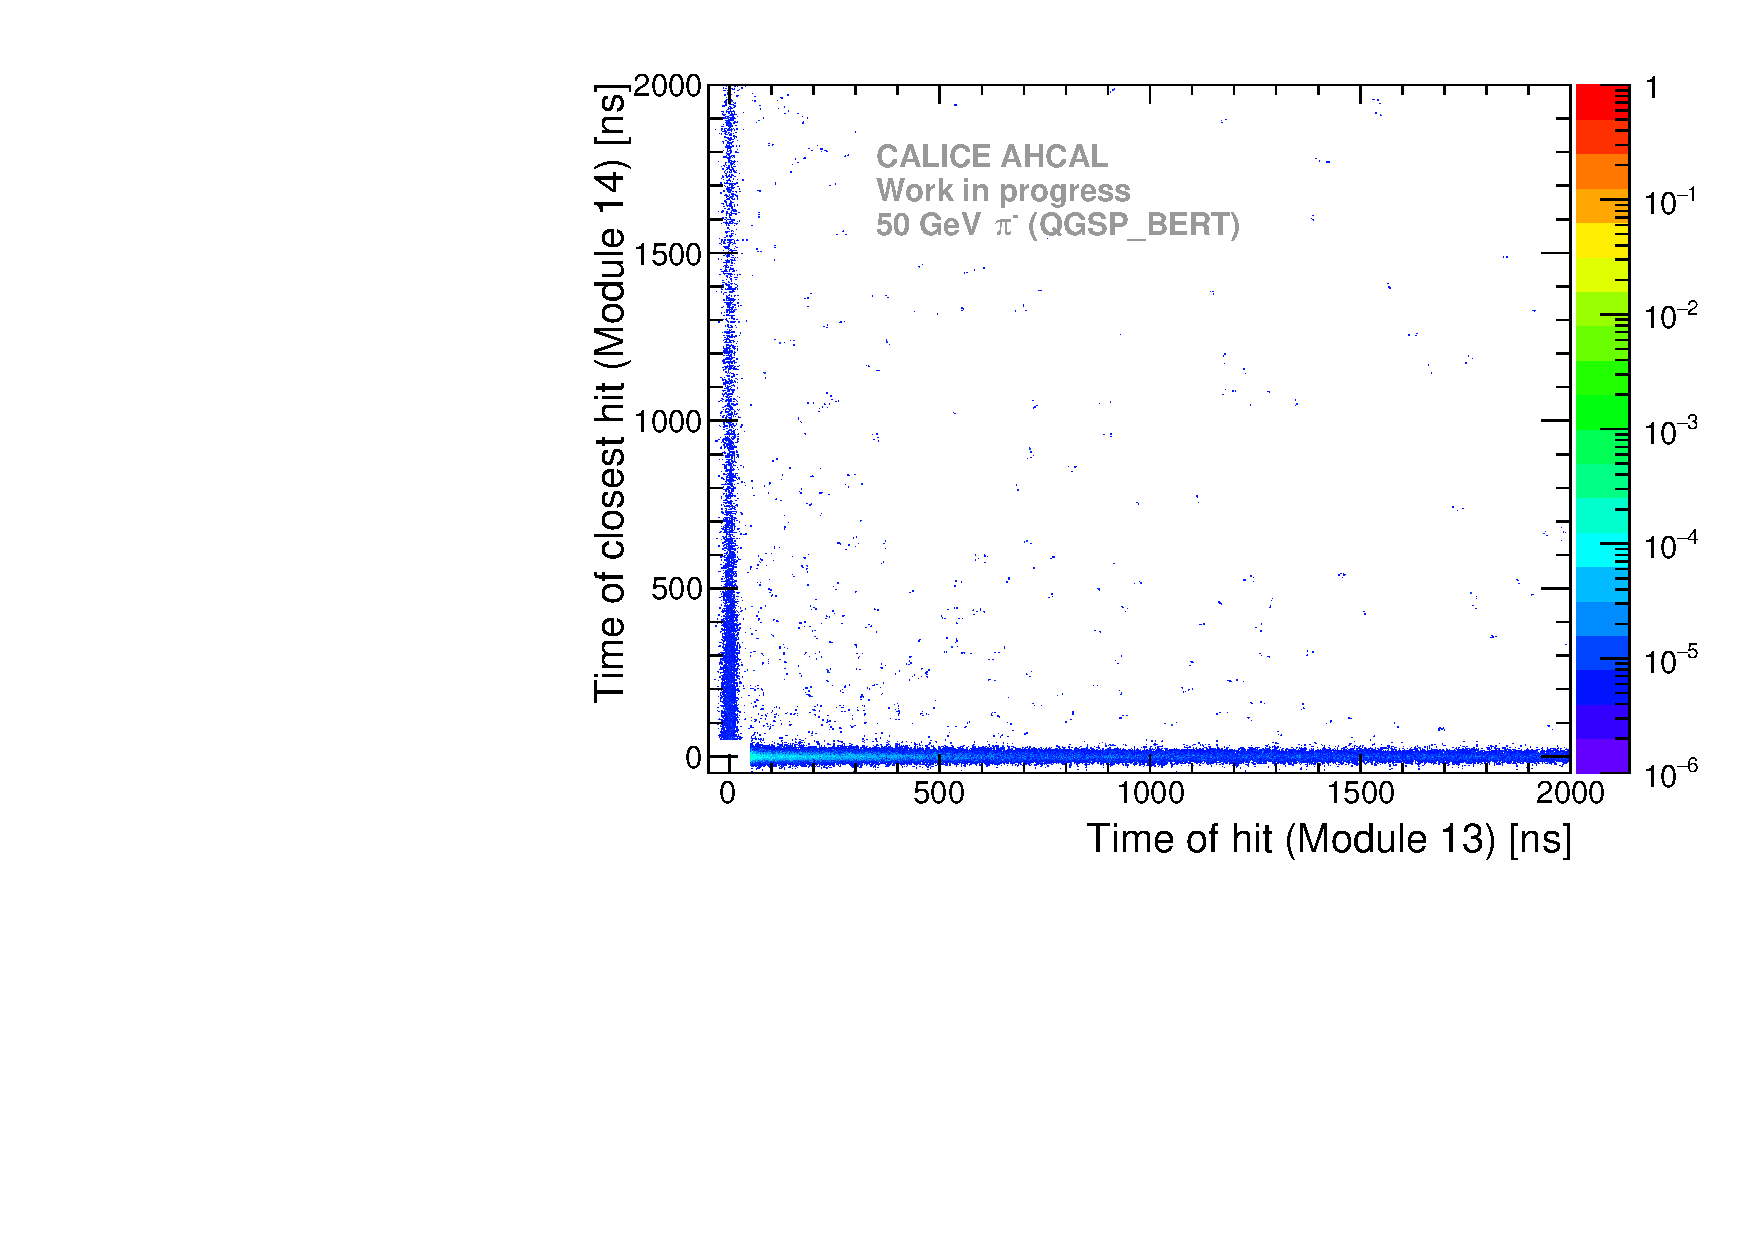
\includegraphics[width=1\textwidth]{chap5/fig_AHCAL_timing/Pions/ComparisonToSim/Time_Correlation_50GeV_long_QGSPBERT.pdf}
		\caption{Long correlation (QGSP\_BERT).} \label{fig:Corr_long_QGSPBERT}
	\end{subfigure}
	\hfill
	\begin{subfigure}[t]{0.5\textwidth}
		\centering
		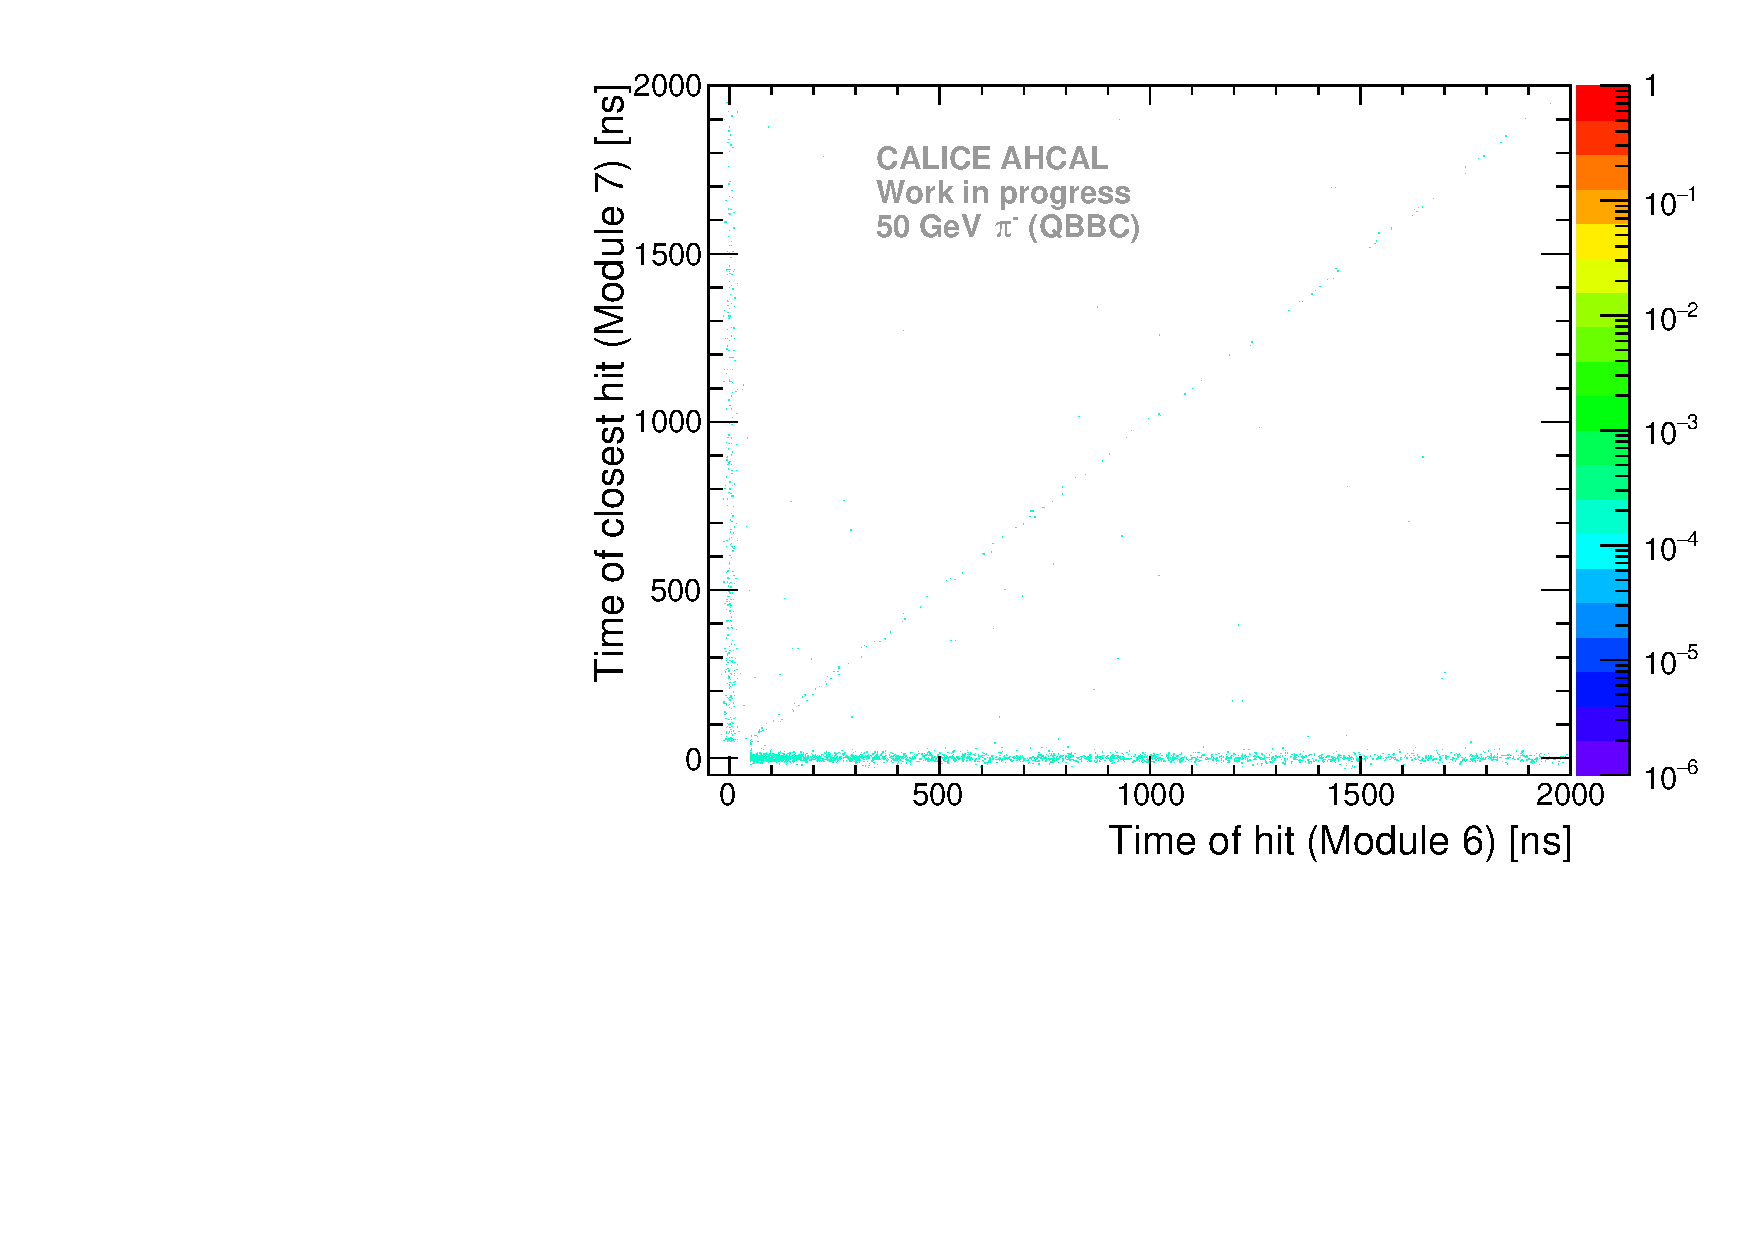
\includegraphics[width=1\textwidth]{chap5/fig_AHCAL_timing/Pions/ComparisonToSim/Time_Correlation_50GeV_short_QBBC.pdf}
		\caption{Short correlation (QBBC).} \label{fig:Corr_short_QBBC}
	\end{subfigure}
	\hfill
	\begin{subfigure}[t]{0.5\textwidth}
		\centering
		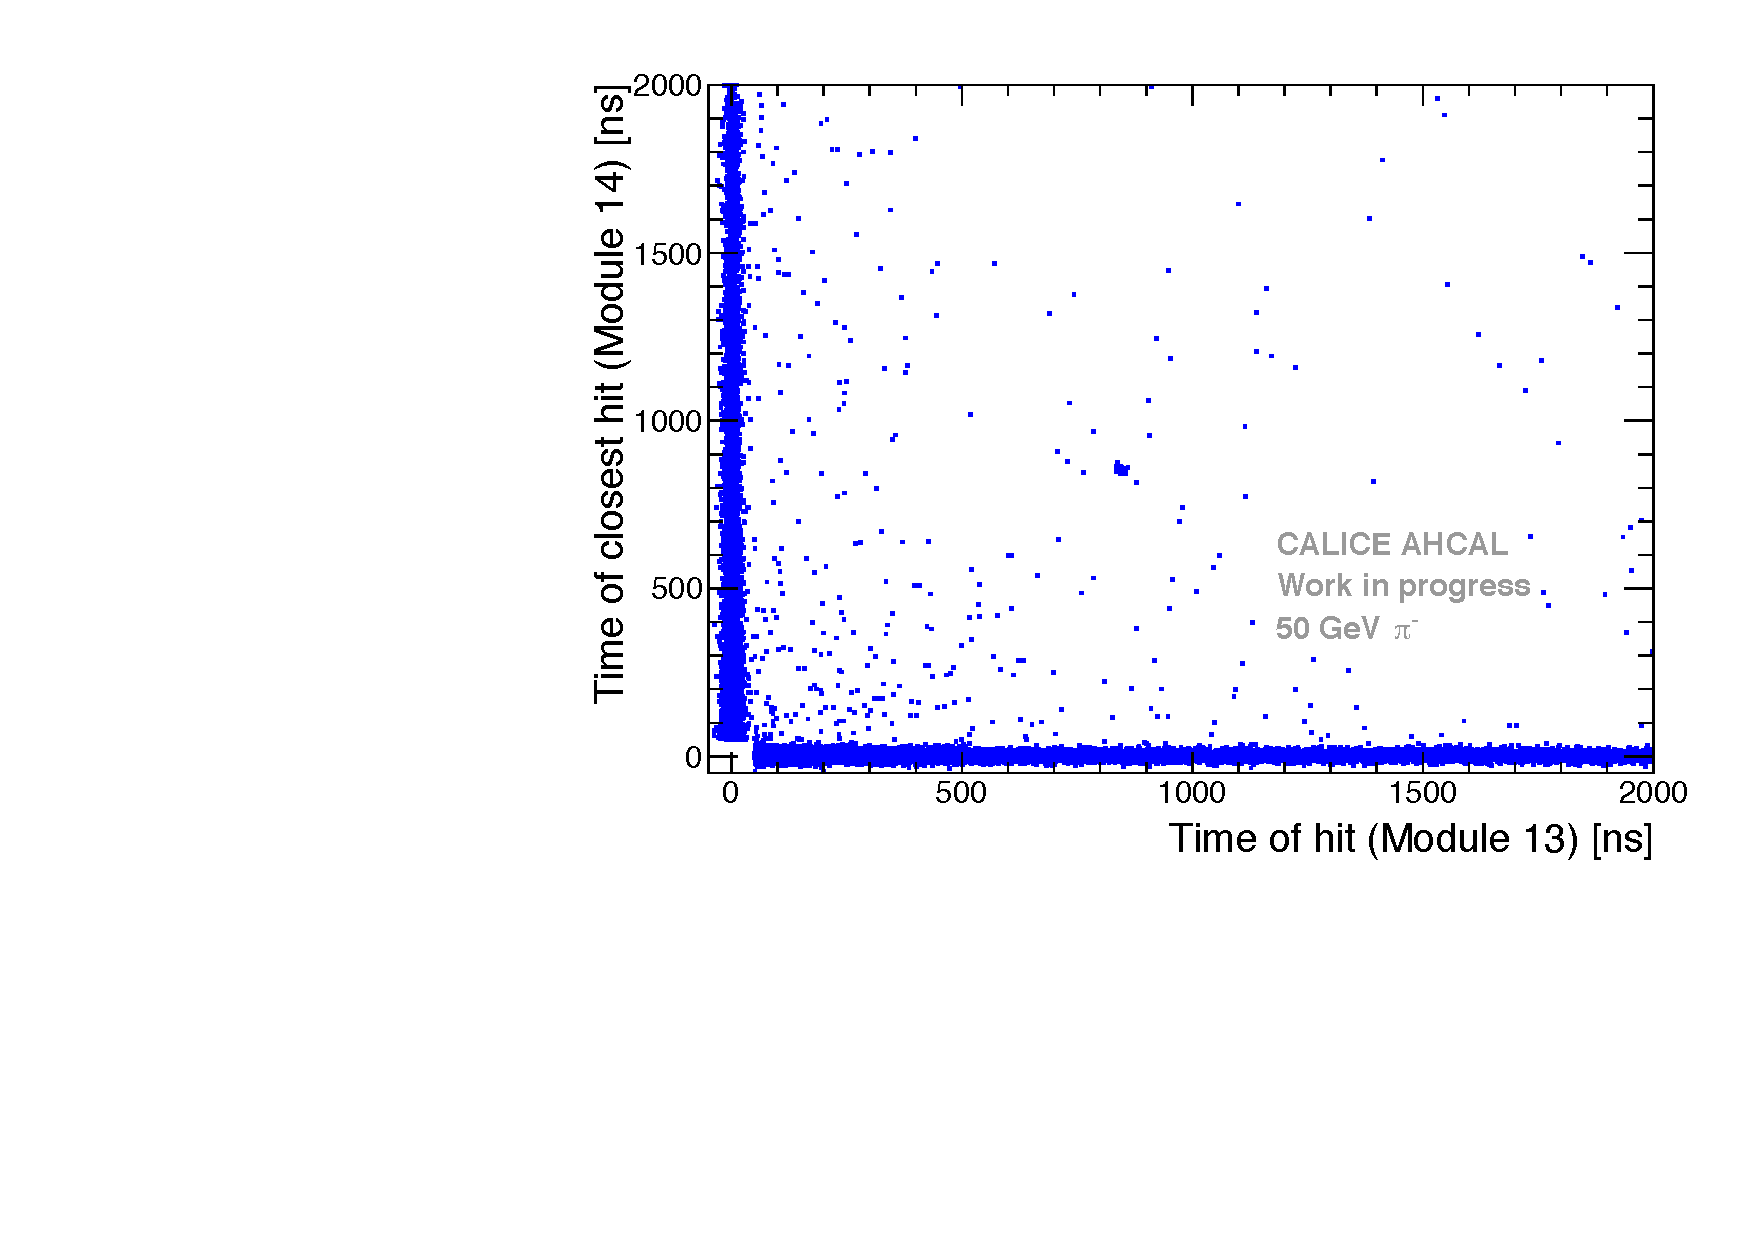
\includegraphics[width=1\textwidth]{chap5/fig_AHCAL_timing/Pions/ComparisonToSim/Time_Correlation_50GeV_long_QBBC.pdf}
		\caption{Long correlation (QBBC).} \label{fig:Corr_long_QBBC}
	\end{subfigure}
	\caption{Timing correlations between layers 6 and 7 and layers 13 and 14 in Mokka simulations for different physics lists in 50 GeV pion beam.}
	\label{fig:Corr_Mokka_Simulation}
\end{figure}
